\documentclass[conference]{IEEEtran}
\IEEEoverridecommandlockouts
% The preceding line is only needed to identify funding in the first footnote. If that is unneeded, please comment it out.

\usepackage{url}
\usepackage{longtable}
\usepackage{ragged2e, tabularx, makecell, booktabs}
\usepackage{tikz, bookmark, tcolorbox, qtree, tikz-qtree}
\usetikzlibrary{shapes.geometric, arrows}
\usepackage[x11names]{xcolor}
\usetikzlibrary{positioning, shapes, arrows.meta,decorations.pathmorphing}

\definecolor{dkgreen}{rgb}{0,0.6,0}
\definecolor{gray}{rgb}{0.5,0.5,0.5}
\definecolor{mauve}{rgb}{0.58,0,0.82}
\usepackage{multirow}
\usepackage{cite}
\usepackage{amsmath,amssymb,amsfonts}
\usepackage{algorithm}
\usepackage{algorithmic}
\usepackage{graphicx}
\usepackage{textcomp}
\usepackage{xcolor}
\usepackage{hyperref}
\def\BibTeX{{\rm B\kern-.05em{\sc i\kern-.025em b}\kern-.08em
    T\kern-.1667em\lower.7ex\hbox{E}\kern-.125emX}}
\begin{document}

\title{A Monte Carlo Tree Search for the
Optimisation of Flight Connections\\
{\large Supplementary Materials (This document is prepared by Arnaud as part of his MSc project)}
}

\author{\IEEEauthorblockN{Arnaud Da Silva\IEEEauthorrefmark{1}, Ahmed Kheiri\IEEEauthorrefmark{1}}
\IEEEauthorblockA{\IEEEauthorrefmark{1}Lancaster University, Department of Management Science, Lancaster LA1 4YX, UK
\\ \{a.dasilva, a.kheiri\}@lancaster.ac.uk}}


\maketitle

\section{Optimisation in Air Travel}

In this section, we discuss some common challenges faced by airline companies and demonstrate the importance of optimisation in decision-making for the success and competitiveness of airline companies.

\subsection{Fleet Assignment Problem}

The Fleet Assignment Problem (FAP), as discussed in \cite{airline_fleet_assignement}, involves assigning different types of aircraft, to flights based on their capabilities, operational costs, and revenue potential. This decision greatly influences airline revenues and is a vital part of the overall scheduling process. The complexity of FAP is driven by the large number of flights an airline manages daily and its interdependencies with other processes like maintenance and crew scheduling.

\subsection{Crew Scheduling Problem} % (fold)

The Crew Scheduling Problem (CSP), as discussed in \cite{crew_scheduling_problem}, involves assigning crews to a sequence of tasks, each with defined start and end times, with the primary objective of ensuring that all tasks are covered while adhering to regulations on maximum working hours for crew members.

This problem is particularly critical for low-cost airlines, for example in the United Kingdom in 2023, low-cost flights comprise 48\% of the scheduled capacity (total number of seats offered) \cite{lcc_new_norm}, which rely heavily on optimised crew schedules to maintain competitiveness. Efficient crew scheduling is essential not only for low cost carriers and for cost minimisation but also for ensuring operational reliability and flexibility in response to unexpected disruptions \cite{ryanair_youtube_report}.


\subsection{Disruption Management} % (fold)
\label{sub:disruption management}

Disruptions in airline operations, as noted in \cite{disruption_management}, can occur due to various factors, including crew unavailability, delays from air traffic control, weather conditions, or mechanical failures. Given that flight schedules are typically planned months in advance \cite{flight_scheduling}, effective disruption management is crucial to minimise the impact on passengers and overall airline operations.

The two mains drivers of disruption management are aircraft and crew recovery.
\begin{itemize}
    \item Aircraft recovery: Optimisation tools help manage the complex logistics of matching available aircraft with rescheduled flights, considering factors like airport availability and maintenance requirements.
    \item Crew recovery: Optimisation tools are used to adjust crew schedules, taking into account factors such as legal working hours, crew availability, and the need to cover all flights efficiently. These tools help in developing feasible and compliant crew rosters that adapt to the new flight schedules.
\end{itemize}

These optimisation strategies, supported by advanced software, for instance \cite{inform_software} and \cite{ibs_software}, are crucial for reducing the impact of disruptions and boosting operational resilience in the airline industry.

\subsection{Airline adaptation to new demand} % (fold)
\label{sub:Airline adaptation to new demand}

Airline companies must continuously adapt their schedules to meet evolving market demands, particularly with the growing dominance of leisure travel over business travel, which has introduced new patterns of demand as shown on Figure \ref{fig:European_demand_seasonality} in Europe. This seasonality poses a challenge for airlines as they have to balance high demand during peak seasons with the risk of underutilisation during off-peak times.

\begin{figure}
    \centering
    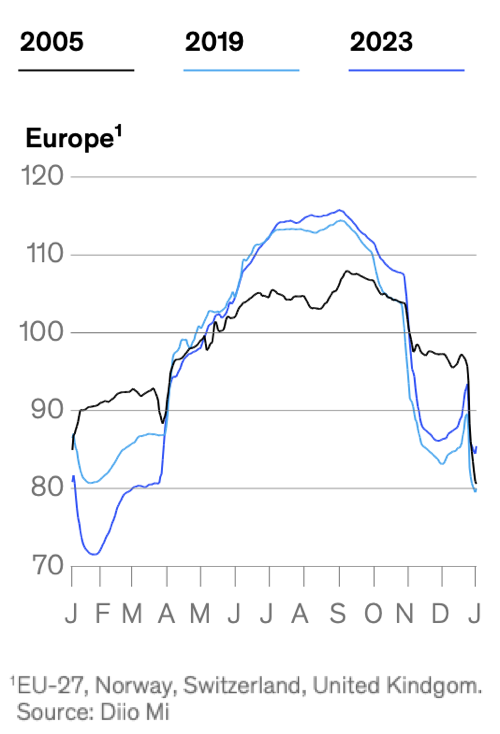
\includegraphics[width=.2\textwidth]{Figures/European Demand.png}
    \caption{European demand seasonality \cite{flight_seasonnality_challenges}}
    \label{fig:European_demand_seasonality}
\end{figure}

Since travel demand varies throughout the year, airlines use a variety of techniques to achieve operational efficiency while maximising revenue \cite{flight_seasonnality_challenges}. For instances, airlines sell nearly 65\% more seats. To ensure their operations remain efficient during periods of heightened demand, airline companies make the required allowance for additional aircraft and crew by optimisation models that specify priority routes and requirements for additional flights, alongside effective crew rotation management.

In contrast, winter months pose a different type of problem where demand drops, which can potentially lead to underutilisation of aircraft. To manage this, airlines are known to turn to ACMI leasing (agreement between two airlines, where the lessor agrees to provide an aircraft, crew, maintenance and insurance \cite{acmi_def}) during periods of low demand to temporarily reduce fleet size by outsourcing their capacity. Alongside this, they also increase maintenance activities and incentivise crews to take holidays or undergo training to maximise productivity across the operation. Equally, on a year-round basis, airlines apply dynamic pricing algorithms to vary fares in reaction to real-time demand patterns. In high-demand summer months, fares are tactically set so as to maximise revenues from travellers willing to pay more, while in winter, pricing strategies are aimed at stimulating demand with fare reductions to fill seats that otherwise would have gone empty. Such adaptive strategies are critical to the airlines for effectively beating the seasonal ebbs and flows in the travel industry.

%\begin{figure}
%    \centering
%    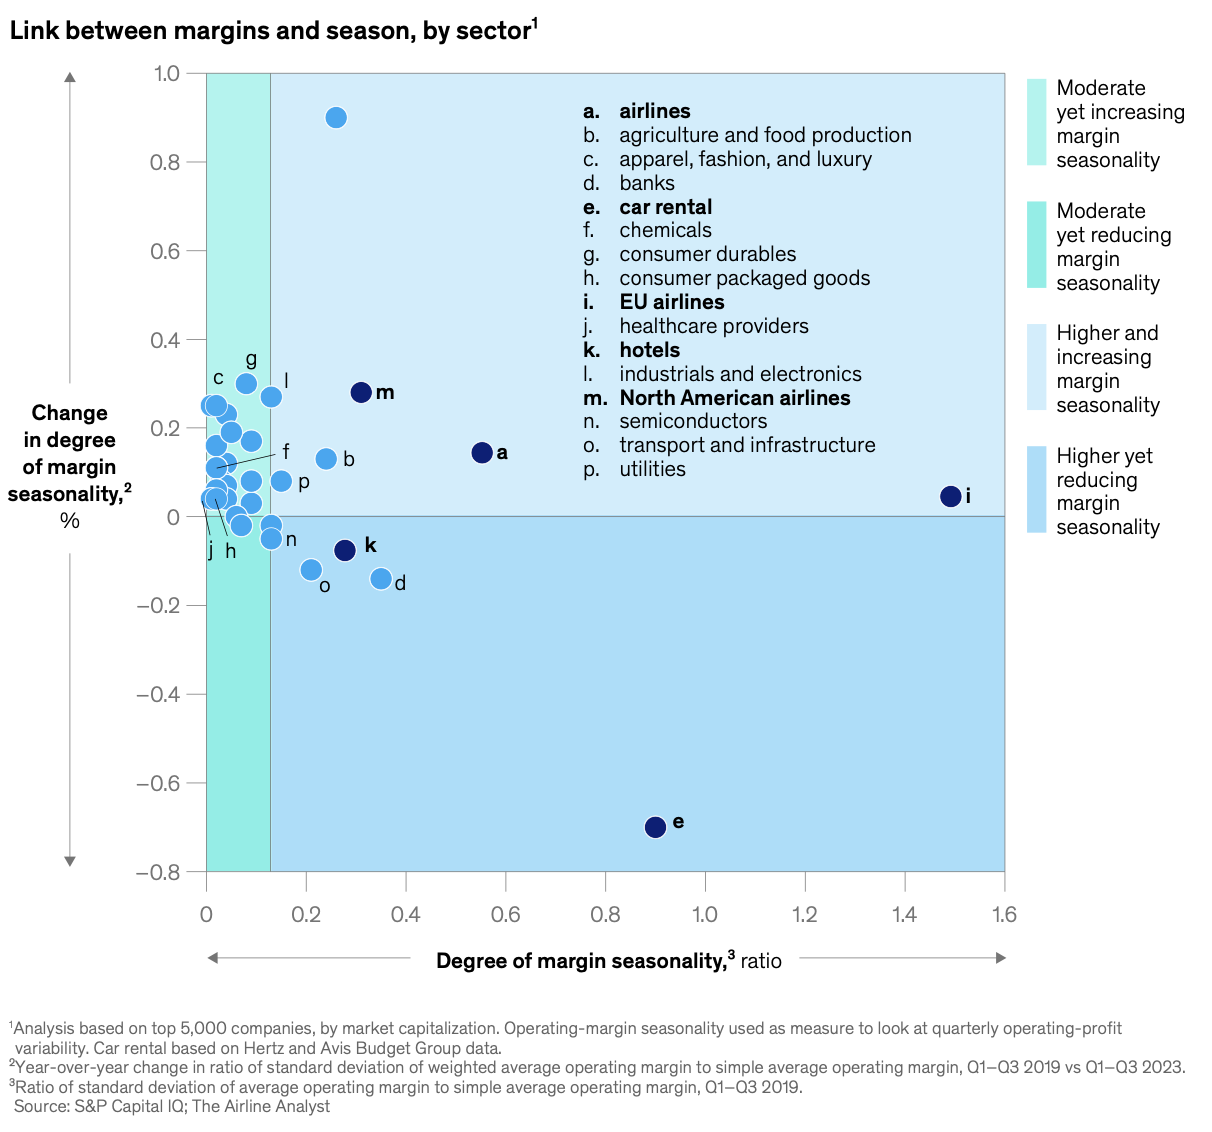
\includegraphics[width=1\textwidth]{Figures/Seasonal margin analysis.png}
%    \caption{Compared with other sectors, airlines exhibit a significant and growing link between margins and seasons.}
%    \label{fig:airline_seasonnality_margin}
%\end{figure}

\section{Travelling Salesman problem and its adaption}
\label{sec:TSP}

The Travelling Salesman Problem is a well known problem in the Operational Research and Computer Science fields. A simple description of the TSP is to find the best round-trip for a salesman that has to travel around a given number of cities while minimising the overall journey's distance. This problem is characterised as $\mathcal{NP}$-Hard \cite{np_hardness}. This means that there is no known polynomial-time algorithm that can solve all instances of the problem efficiently. Regarding time complexity, if we were to solve it exploring all the possible solutions, the time complexity would have been $\mathcal{O}(\frac{(n-1)!}{2})$ where $n$ represents the number of cities.

\begin{figure}
    \centering
    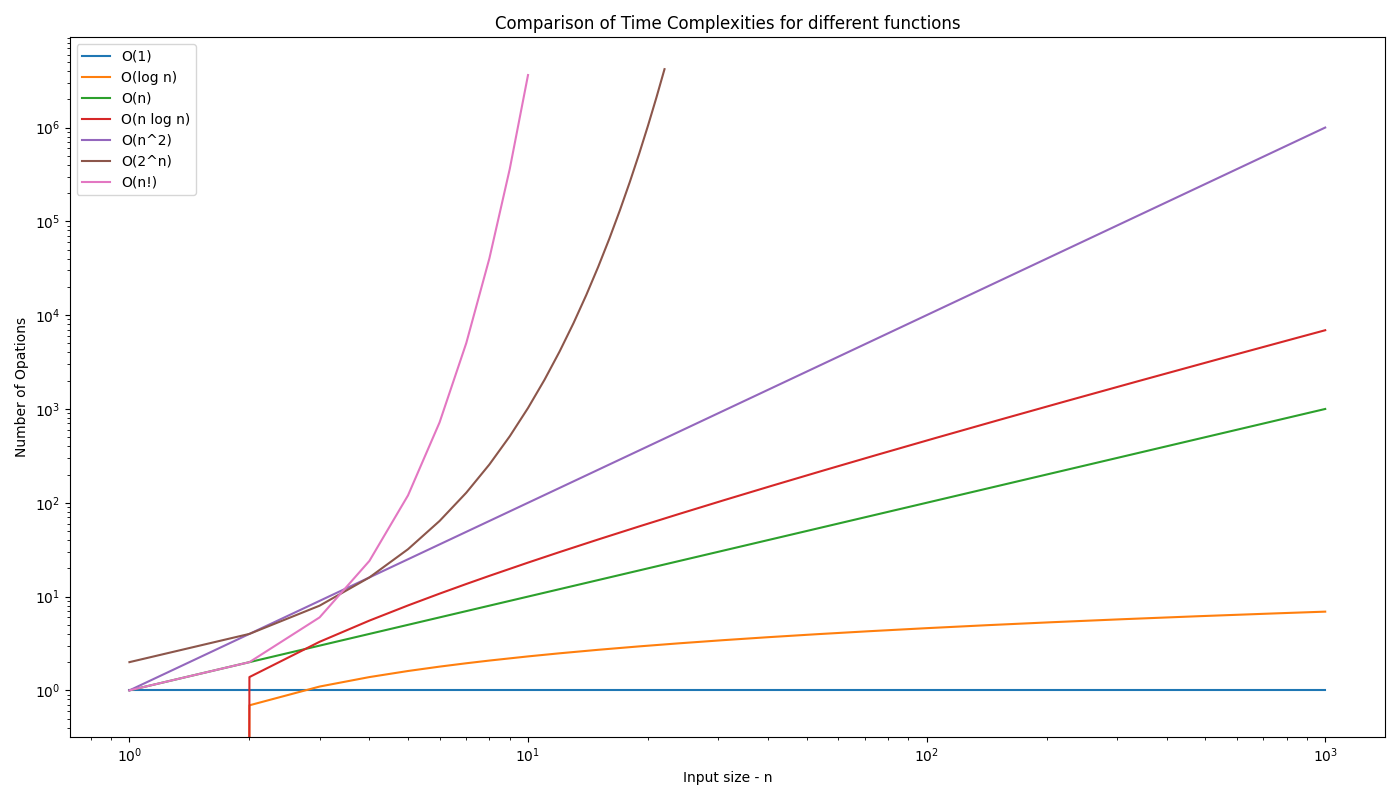
\includegraphics[width=0.48\textwidth]{Figures/Time_complexities.png}
    \caption{Time complexity of different functions}
    \label{fig:time_complexity_comparisons}
\end{figure}

On Figure \ref{fig:time_complexity_comparisons}, different time complexities are compared and demonstrates that the factorial time complexity is the worst. Therefore, these kinds of $\mathcal{NP}$-Hard problem are typically not solved by exploiting all the search area but using heuristics algorithms. Heuristic solutions do not guarantee to find the absolute optimal solution but can find near-optimal solutions within more reasonable timeframes.

The TSP has been studied extensively, and, many variants can be derived from it:

\begin{itemize}
    \item Symmetric TSP (STSP): The distance between cities are symmetric, meaning that the distance to travel from city A to city B is the same as from city B to city A. %\cite{STSP}
    \item Asymmetric TSP (ATSP): The distance between cities are asymmetric, meaning that the distance to travel from city A to city B is different than the distance to travel from city B to city A \cite{ASTP}.
    \item Multiple TSP (mTSP): Instead of one salesman, multiple salesman are starting from one city, they visit all the cities such that each city is visited exactly once \cite{mTSP}.
    \item Time Window TSP (TWTSP): Each city has to be visited in a defined time slot \cite{TWTSP}.
    \item Price-collection TSP (PCTSP): Not all the cities have to be visited, the goal is to minimise the overall traveller's distance while maximising the price collected earned when visiting a city \cite{PCTSP}.
    \item Stochastic TSP (STSP): The distances between the cities or the cost of travels are stochastic (i.e., random variables) rather than deterministic \cite{Stochastic_TSP}.
    \item Dynamic TSP (DTSP): The problem can change over time, that means that new cities can be added or distances between cities can change while the salesman has already started his journey \cite{DTSP}.
    \item Generalised TSP (GTSP): The cities are grouped into clusters, the goal is to visit exactly one city from each cluster \cite{GTSP}.
    \item Open TSP (OTSP): The traveller does not have to end his journey at the starting city \cite{OTSP}.
\end{itemize}

Multiple algorithms have been developed to address these TSP variants, we can classify them into two categories:

\begin{itemize}
    \item \textbf{Exact algorithms}: These algorithms aim to find the optimal solution to the TSP by exploring all possible routes or by using mathematical techniques to prune the search space efficiently.
          \begin{itemize}
              \item \textbf{Branch and Bound}: This method systematically explores the set of all possible solutions, using bounds to eliminate parts of the search space that cannot contain the optimal solution. It is often used for smaller instances of TSP \cite{branch_and_bound}.
              \item \textbf{Cutting planes}: This technique adds constraints (or cuts) to the TSP formulation iteratively to remove infeasible solutions and converge to the optimal solution. This approach is particularly effective for symmetric TSPs \cite{cutting_planes}.
              \item \textbf{Dynamic Programming}: Introduced by Bellman, this approach breaks down the TSP into subproblems and solves them recursively, and despite its exponential complexity it is highly effective for solving some TSP variants \cite{dynamic_programming_tsp}.
          \end{itemize}
    \item \textbf{Heuristic Algorithms}: These algorithms are designed to find near-optimal solutions within a reasonable timeframe, specifically for large-scale problems where exact methods are computationally infeasible.
          \begin{itemize}
              \item \textbf{Greedy Algorithms}: These algorithms make a series of locally optimal choices in the hope of finding a global optimum. An example is the Nearest Neighbour algorithm, which selects the nearest unvisited city at each step \cite{greedy}.
              \item \textbf{Genetic Algorithms}: Inspired by the process of natural selection, these algorithms evolve a population of solutions over time, using operations such as mutation and crossover to explore the solution space \cite{genetic_algorithm}.
              \item \textbf{Simulated Annealing}: This probabilistic technique searches for a global optimum by allowing worsening moves to be accepted based on a temperature parameter that gradually decreases. It is particularly useful for escaping local optima \cite{simulated_annealing}.
              \item \textbf{Ant Colony Optimisation}: This metaheuristic is inspired by the foraging behaviour of ants and uses a combination of deterministic and probabilistic rules to construct solutions, which are gradually refined through updates based on pheromone trails \cite{ant_colony}.
          \end{itemize}
\end{itemize}

\section{Monte Carlo Tree Search algorithm}

The Monte Carlo Tree Search (MCTS) algorithm can be characterised as less traditional than the methods described in Section \ref{sec:TSP} to solve TSP problems. MCTS and its variants have been successfully implemented across a range of games, such as Havannah \cite{wiki:board_game}, Amazons \cite{wiki:Game_of_the_Amazons}, Lines of Actions \cite{wiki:Lines_of_Action}, Go, Chess, and Shogi \cite{wiki:Shogi}, establishing it as the state-of-the-art algorithm \cite{havannah,amazons,lines_of_actions}. It is widely used in board games and is increasingly popular since Google DeepMind developed AlphaGo. AlphaGo is a software that was created to beat the best Go's player in the world. Go is a board game from China where two players take turns placing black or white stones on a grid. The goal is to capture territory by surrounding empty spaces or the opponent's stones. Despite its simple rules, Go is a complex game, with countless possible moves and strategies. It is known for its balance between intuition and logic, hence why it has been a significant focus of artificial intelligence research \cite{wiki:Go}. In 2016, Lee Sedol \cite{wiki:Lee_Sedol}, the best Go's player in the world was been beaten by AlphaGo 4-1 \cite{alpha_go_documentary}. MCTS with policy and value networks are at the heart of AlphaGo decision-making process, enabling AlphaGo's to pick the optimal moves in the complex search of Go \cite{mcts_alpha_go_algorithm}.

\subsection{Overview}

The MCTS' process is conceptually straightforward. A tree is built in an incremental and asymmetric manner (Figure \ref{fig:Assymetrical_growth_MCTS}).
For every iteration, a selection policy is used to determine which node to select in the tree to perform simulations. 
The selection policy, typically balances the exploration  (looking into parts of the tree that have not been visited yet) and the exploitation (looking into parts of the trees that appear to be promising). 
Once the node is selected, a simulation (a sequence of available actions, based on a simulation policy), is applied from this node until a terminal condition is reached (e.g., no further actions are possible) \cite{mcts_various_policies}.

\begin{figure}
    \centering
    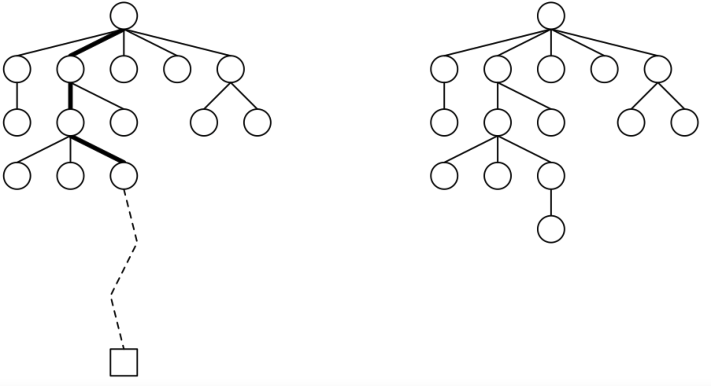
\includegraphics[width=0.5\textwidth]{Figures/assymetric_growth_mcts_tree.png}
    \caption{Assymetrical growth of MCTS - Simulation and Expansion - \cite{mcts_assymetrical_growth}}
    \label{fig:Assymetrical_growth_MCTS}
\end{figure}


To ensure a clearer understanding of MCTS algorithm's stages, we will start by exploring a detailed example \cite{example_youtube_mcts}. This example will illustrate each component of the algorithm in action. Furthermore, we will generalise the principles discussed, as the methodology of this paper is built on the application of the MCTS algorithm.

Considering a maximisation problem, when starting a game, the player can choose between two possible actions $a_1$ and $a_2$ from the node $S^{0,0}_0$ in the tree $\mathcal{T}$. 
Every node is defined like so: $S^{n_i,t_i}_i$ where $n_i$ represents the number of times node $i$ has been visited, $t_i$ the total score of this node.
Moreover, for every node - a selection metric can be computed, for instance the $UCB$ value: $UCB(S^{n_i,t_i}_i)=\bar{V_i} + 2 \sqrt{\frac{\ln N}{n_i}}$ where $\bar{V_i}=\frac{n_i}{t_i}$ represents the average value of the node, $n_i$ the number of times node $i$ has been visited, $N=n_0$ the number of times the root node has been visited (which is also equal to the number of iterations).

Before the first iteration, $I_{t1}$, none node has been visited - $\forall i \in \mathcal{T}, S^{0,0}_{i}$.
\begin{figure}
    \centering
    \scalebox{0.8}{
    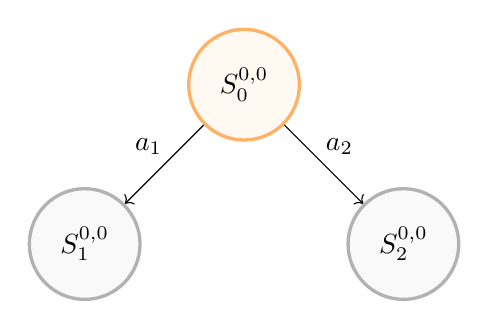
\begin{tikzpicture}[
            root_node/.style={circle, draw=orange!60, fill=orange!5, very thick, minimum size=40},
            visited_node/.style={circle, draw=green!60, fill=green!5, very thick, minimum size=40},
            unvisited_node/.style={circle, draw=gray!60, fill=gray!5, very thick, minimum size=40},
            target_node/.style={circle, draw=green!60, fill=green!5, very thick, minimum size=40},
        ]

        \node[root_node](Root){$S^{0,0}_0$};
        \node[unvisited_node, below left=of Root](S1){$S^{0,0}_1$};
        %\node[target_node, below=of S1, yshift=-1.7cm](Target){};
        \node[unvisited_node, below right=of Root](S2){$S^{0,0}_2$};

        \draw[->] (Root) -- (S1) node[midway, above, xshift=-2mm] {$a_1$};
        \draw[->] (Root) -- (S2) node[midway, above, xshift=2mm] {$a_2$};

        %\draw[->, very thick, decorate, decoration={snake, amplitude=.7mm, segment length=3mm}] (S1) -- (Target);
    \end{tikzpicture}
    }
    \caption{Selection - $I_{t1}$}
    \label{fig:Expansion of the tree from the root node}
\end{figure}

At the beginning of $I_{t1}$, the player has to choose between these two child nodes (or choose between taking $a_1$ or $a_2$). After, the player has to calculate the $UCB$ value for these two nodes and pick the node that maximises the $UCB$ value (as it is a maximisation problem).
In Figure \ref{fig:Expansion of the tree from the root node}, neither of these have been visited yet so $UCB(S^{0,0}_1)=UCB(S^{0,0}_2)=\infty$. Hence, the player decides to choose randomly $S^{0,0}_1$.

$S^{0,0}_1$ is a leaf node that has not been visited, then a simulation can be done from this node. It means selecting actions from this node based on the simulation policy to a terminal state as shown on Figure \ref{fig:Simulation - $I1$}:

\begin{figure}
    \centering
    \scalebox{0.8}{
    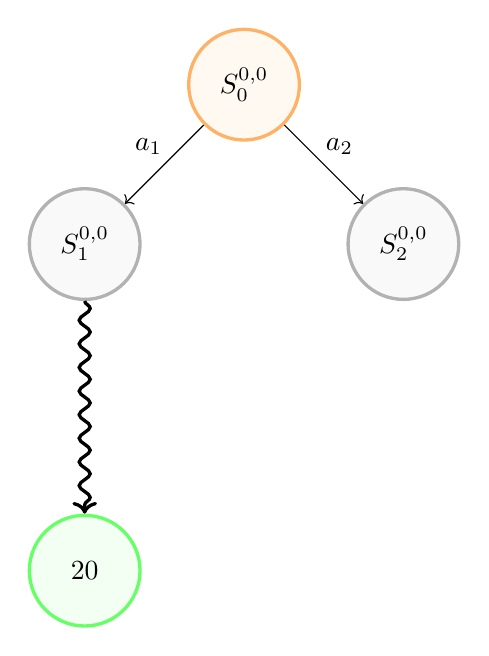
\begin{tikzpicture}[
            root_node/.style={circle, draw=orange!60, fill=orange!5, very thick, minimum size=40},
            visited_node/.style={circle, draw=green!60, fill=green!5, very thick, minimum size=40},
            unvisited_node/.style={circle, draw=gray!60, fill=gray!5, very thick, minimum size=40},
            target_node/.style={circle, draw=green!60, fill=green!5, very thick, minimum size=40},
        ]

        \node[root_node](Root){$S^{0,0}_0$};
        \node[unvisited_node, below left=of Root](S1){$S^{0,0}_1$};
        \node[target_node, below=of S1, yshift=-1.7cm](Target){20};
        \node[unvisited_node, below right=of Root](S2){$S^{0,0}_2$};

        \draw[->] (Root) -- (S1) node[midway, above, xshift=-2mm] {$a_1$};
        \draw[->] (Root) -- (S2) node[midway, above, xshift=2mm] {$a_2$};

        \draw[->, very thick, decorate, decoration={snake, amplitude=.7mm, segment length=3mm}] (S1) -- (Target);
    \end{tikzpicture}
    }
    \caption{Simulation - $I_{t1}$}
    \label{fig:Simulation - $I1$}
\end{figure}

The terminal state has a value of 20, we can write that the rollout/simulation from node $S^{0,0}_1$ is $\mathcal{R}(S^{0,0}_1)=20$ . The final step of $I_{t1}$ is backpropagation. Every node that has been visited in the iteration is updated.
Let $\mathcal{N}_{\mathcal{R},j}$ be the indices of the nodes visited during the $j-th$ iteration of the MCTS:
\begin{itemize}
    \item Before backpropagation:
          \begin{equation}
              \forall i \in \mathcal{N}_{\mathcal{R},j}, S^{n_i,t_i}_{i,old}
          \end{equation}

    \item After backpropagation:
          \begin{equation}
              \forall i \in \mathcal{N}_{\mathcal{R},j}, S^{n_i+1,t_i+\mathcal{R}(S^{n_i,t_i}_{i,old})}_{i,new}
          \end{equation}
\end{itemize}

We can then define a backpropagation function:
\begin{center}
    \centering
    $\begin{array}{ccccc}
            \mathcal{B} & : & \mathcal{N}_{\mathcal{R},j} & \to     & \mathcal{N}_{\mathcal{R},j}                    \\
                        &   & S^{n_i,t_i}_{i}             & \mapsto & S^{n_i+1,t_i+\mathcal{R}(S^{n_i,t_i}_{i})}_{i} \\
        \end{array}$
\end{center}

Then, back to the example on Figure \ref{fig:Backpropagation_I1}, the player updates the visited nodes: $\mathcal{B}(S^{0,0}_1)=S^{\mathbf{1},\mathbf{20}}_1$ and $\mathcal{B}(S^{0,0}_0)=S^{\mathbf{1},\mathbf{20}}_0$.
\begin{figure}
    \centering
    \scalebox{0.8}{
    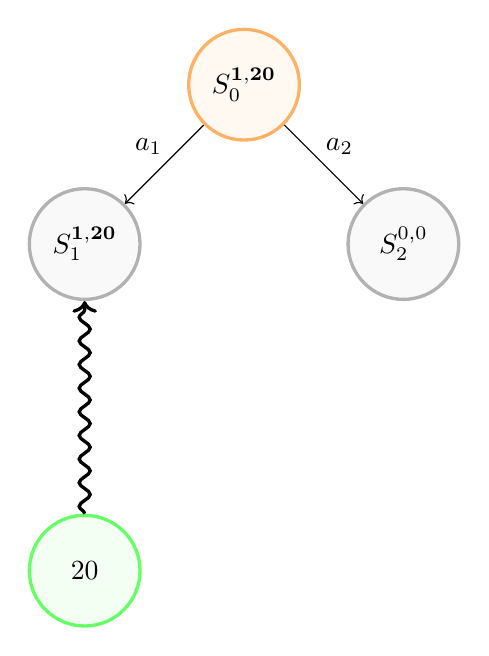
\begin{tikzpicture}[
            root_node/.style={circle, draw=orange!60, fill=orange!5, very thick, minimum size=40},
            visited_node/.style={circle, draw=green!60, fill=green!5, very thick, minimum size=40},
            unvisited_node/.style={circle, draw=gray!60, fill=gray!5, very thick, minimum size=40},
            target_node/.style={circle, draw=green!60, fill=green!5, very thick, minimum size=40}
        ]

        \node[root_node](Root){$S^{\mathbf{1},\mathbf{20}}_0$};
        \node[unvisited_node, below left=of Root](S1){$S^{\mathbf{1},\mathbf{20}}_1$};
        \node[target_node, below=of S1, yshift=-1.7cm](Target){20};
        \node[unvisited_node, below right=of Root](S2){$S^{0,0}_2$};

        \draw[->] (Root) -- (S1) node[midway, above, xshift=-2mm] {$a_1$};
        \draw[->] (Root) -- (S2) node[midway, above, xshift=2mm] {$a_2$};

        \draw[->, very thick, decorate, decoration={snake, amplitude=.7mm, segment length=3mm}] (Target) -- (S1);
    \end{tikzpicture}
    }
    \caption{Backpropagation - $I_{t1}$}
    \label{fig:Backpropagation_I1}
\end{figure}

The fourth phase of the algorithm has been done for $I_{t1}$. Therefore, the player can start the $2^{nd}$ iteration of the MCTS, $I_{t2}$.

\begin{figure}
    \centering
    \scalebox{0.7}{
    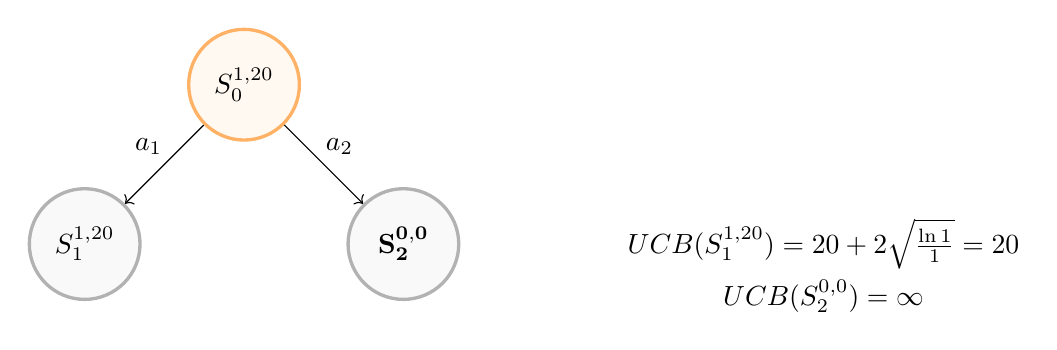
\begin{tikzpicture}[
            root_node/.style={circle, draw=orange!60, fill=orange!5, very thick, minimum size=40},
            visited_node/.style={circle, draw=green!60, fill=green!5, very thick, minimum size=40},
            unvisited_node/.style={circle, draw=gray!60, fill=gray!5, very thick, minimum size=40},
            target_node/.style={circle, draw=green!60, fill=green!5, very thick, minimum size=40}
        ]

        \node[root_node](Root){$S^{1,20}_0$};
        \node[unvisited_node, below left=of Root](S1){$S^{1,20}_1$};
        %\node[target_node, below=of S1, yshift=-1.7cm](Target){20};
        \node[unvisited_node, below right=of Root](S2){$\mathbf{S^{0,0}_2}$};

        \node[right=2cm of S2, anchor=west] (UCB) {$UCB(S^{1,20}_1)=20+2 \sqrt{\frac{\ln1}{1}} = 20$};
        \node[below=0.55cm of UCB, anchor=south] (UCB2) {$UCB(S^{0,0}_2)=\infty$};

        \draw[->] (Root) -- (S1) node[midway, above, xshift=-2mm] {$a_1$};
        \draw[->] (Root) -- (S2) node[midway, above, xshift=2mm] {$a_2$};

        %\draw[->, very thick, decorate, decoration={snake, amplitude=.7mm, segment length=3mm}] (S1) -- (Target);
    \end{tikzpicture}
    }
    \caption{Selection - $I_{t2}$}
    \label{fig:Selection - I2}
\end{figure}

On Figure \ref{fig:Selection - I2}, the player can either choose $a_1$ or $a_2$. When a child node has not been visited yet, the player picks this node for the Selection iteration, or they can compute the $UCB$ value, it leads to the same conclusion.

\begin{figure}
    \centering
    \scalebox{0.8}{
    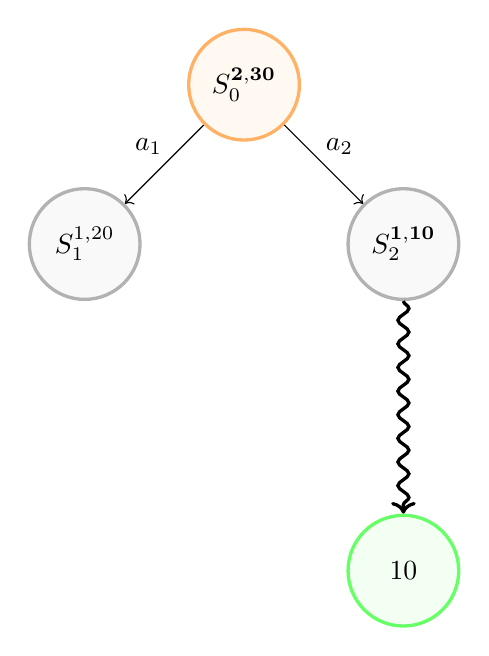
\begin{tikzpicture}[
            root_node/.style={circle, draw=orange!60, fill=orange!5, very thick, minimum size=40},
            visited_node/.style={circle, draw=green!60, fill=green!5, very thick, minimum size=40},
            unvisited_node/.style={circle, draw=gray!60, fill=gray!5, very thick, minimum size=40},
            target_node/.style={circle, draw=green!60, fill=green!5, very thick, minimum size=40},
        ]

        \node[root_node](Root){$S^{\mathbf{2},\mathbf{30}}_0$};
        \node[unvisited_node, below left=of Root](S1){$S^{1,20}_1$};

        \node[unvisited_node, below right=of Root](S2){$S^{\mathbf{1},\mathbf{10}}_2$};
        \node[target_node, below=of S2, yshift=-1.7cm](Target){10};

        \draw[->] (Root) -- (S1) node[midway, above, xshift=-2mm] {$a_1$};
        \draw[->] (Root) -- (S2) node[midway, above, xshift=2mm] {$a_2$};

        \draw[->, very thick, decorate, decoration={snake, amplitude=.7mm, segment length=3mm}] (S2) -- (Target);
    \end{tikzpicture}
    }
    \caption{Simulation and Backpropagation - $I_{t2}$}
    \label{fig:Simulation and Backpropagation - I2}
\end{figure}


A simulation is executed (Figure \ref{fig:Simulation and Backpropagation - I2}) from the chosen node $S^{0,0}_{2}$ and $\mathcal{R}(S^{0,0}_{2})=10$ and then the outcome is backpropagated to all the visited nodes: $\mathcal{B}(S^{0,0}_{2})=S^{1,10}_{2}$ and $\mathcal{B}(S^{1,20}_{0})=S^{2,30}_{0}$. Next, $I_{t3}$ starts, based on the $UCB$ score, the player chooses $a_1$.

\begin{figure}
    \centering
    \scalebox{0.8}{
    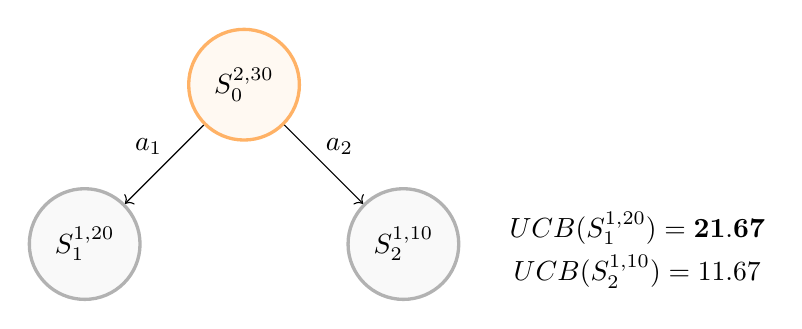
\begin{tikzpicture}[
            root_node/.style={circle, draw=orange!60, fill=orange!5, very thick, minimum size=40},
            visited_node/.style={circle, draw=green!60, fill=green!5, very thick, minimum size=40},
            unvisited_node/.style={circle, draw=gray!60, fill=gray!5, very thick, minimum size=40},
            target_node/.style={circle, draw=green!60, fill=green!5, very thick, minimum size=40},
        ]

        \node[root_node](Root){$S^{2,30}_0$};
        \node[unvisited_node, below left=of Root](S1){$S^{1,20}_1$};

        \node[unvisited_node, below right=of Root](S2){$S^{1,10}_2$};
        %\node[target_node, below=of S2, yshift=-1.7cm](Target){10};
        \node[right=5mm of S2, anchor=west, yshift=2mm] (UCB) {$UCB(S^{1,20}_1)=\mathbf{21.67}$};
        \node[below=0.55cm of UCB, anchor=south] (UCB2) {$UCB(S^{1,10}_2)=11.67$};

        \draw[->] (Root) -- (S1) node[midway, above, xshift=-2mm] {$a_1$};
        \draw[->] (Root) -- (S2) node[midway, above, xshift=2mm] {$a_2$};

        %\draw[->, very thick, decorate, decoration={snake, amplitude=.7mm, segment length=3mm}] (S2) -- (Target);
    \end{tikzpicture}
    }
    \caption{Selection - $I_{t3}$}
    \label{fig:Selection - I3}
\end{figure}


$S^{1,20}_{1}$ is a leaf node and has been visited, this node can be expanded.

\begin{figure}
\scalebox{0.8}{
    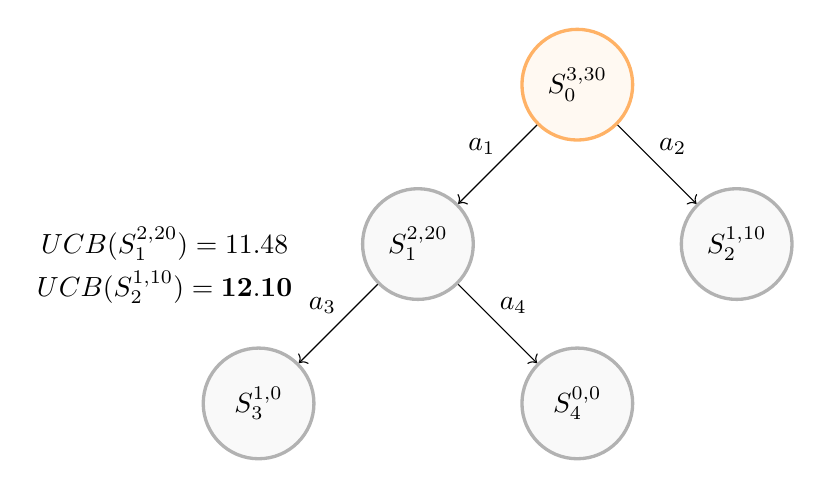
\begin{tikzpicture}[
            root_node/.style={circle, draw=orange!60, fill=orange!5, very thick, minimum size=40},
            visited_node/.style={circle, draw=green!60, fill=green!5, very thick, minimum size=40},
            unvisited_node/.style={circle, draw=gray!60, fill=gray!5, very thick, minimum size=40},
            target_node/.style={circle, draw=green!60, fill=green!5, very thick, minimum size=40},
        ]

        \node[root_node](Root){$S^{3,30}_0$};
        \node[unvisited_node, below left=of Root](S1){$S^{2,20}_1$};
        \node[unvisited_node, below right=of Root](S2){$S^{1,10}_2$};
        \node[unvisited_node, below left=of S1](S3){$S^{1,0}_3$};
        \node[unvisited_node, below right=of S1](S4){$S^{0,0}_4$};

        \node[left=8mm of S1, anchor=east] (UCB) {$UCB(S^{2,20}_1)=11.48$};
        \node[below=0.55cm of UCB, anchor=south] (UCB2) {$UCB(S^{1,10}_2)=\mathbf{12.10}$};

        %\node[target_node, below=of S3, yshift=-1.7cm](Target){0};

        \draw[->] (Root) -- (S1) node[midway, above, xshift=-2mm] {$a_1$};
        \draw[->] (Root) -- (S2) node[midway, above, xshift=2mm] {$a_2$};
        \draw[->] (S1) -- (S3)   node[midway, above, xshift=-2mm] {$a_3$};
        \draw[->] (S1) -- (S4)   node[midway, above, xshift=2mm] {$a_4$};
        %\draw[->, very thick, decorate, decoration={snake, amplitude=.7mm, segment length=3mm}] (S3) -- (Target);
    \end{tikzpicture}
    }
    \caption{Selection and Expansion - $I_{t3}$}
\end{figure}

Based on $UCB$ score, a simulation is done from $S^{0,0}_3$ on Figure \ref{fig:Simulation and Backpropagation - I3}.

\begin{figure}
    \centering
    \scalebox{0.8}{
    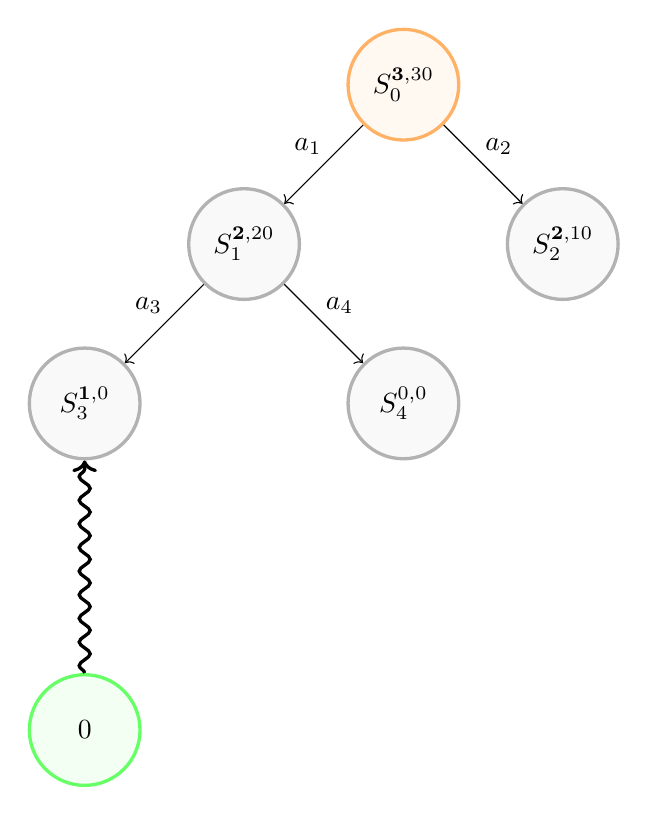
\begin{tikzpicture}[
            root_node/.style={circle, draw=orange!60, fill=orange!5, very thick, minimum size=40},
            visited_node/.style={circle, draw=green!60, fill=green!5, very thick, minimum size=40},
            unvisited_node/.style={circle, draw=gray!60, fill=gray!5, very thick, minimum size=40},
            target_node/.style={circle, draw=green!60, fill=green!5, very thick, minimum size=40},
        ]

        \node[root_node](Root){$S^{\mathbf{3},30}_0$};
        \node[unvisited_node, below left=of Root](S1){$S^{\mathbf{2},20}_1$};
        \node[unvisited_node, below right=of Root](S2){$S^{\mathbf{2},10}_2$};
        \node[unvisited_node, below left=of S1](S3){$S^{\mathbf{1},0}_3$};
        \node[unvisited_node, below right=of S1](S4){$S^{0,0}_4$};

        \node[target_node, below=of S3, yshift=-1.7cm](Target){0};

        \draw[->] (Root) -- (S1) node[midway, above, xshift=-2mm] {$a_1$};
        \draw[->] (Root) -- (S2) node[midway, above, xshift=2mm] {$a_2$};
        \draw[->] (S1) -- (S3)   node[midway, above, xshift=-2mm] {$a_3$};
        \draw[->] (S1) -- (S4)   node[midway, above, xshift=2mm] {$a_4$};
        \draw[->, very thick, decorate, decoration={snake, amplitude=.7mm, segment length=3mm}] (Target) -- (S3);
    \end{tikzpicture}
    }
    \caption{Simulation and Backpropagation - $I_{t3}$}
    \label{fig:Simulation and Backpropagation - I3}
\end{figure}


This is the fourth iteration, $I_{t4}$ represented on Figure \ref{fig:Selection - Simulation - Backpropagation - I4}.

\begin{figure}
    \centering
    \scalebox{0.8}{
    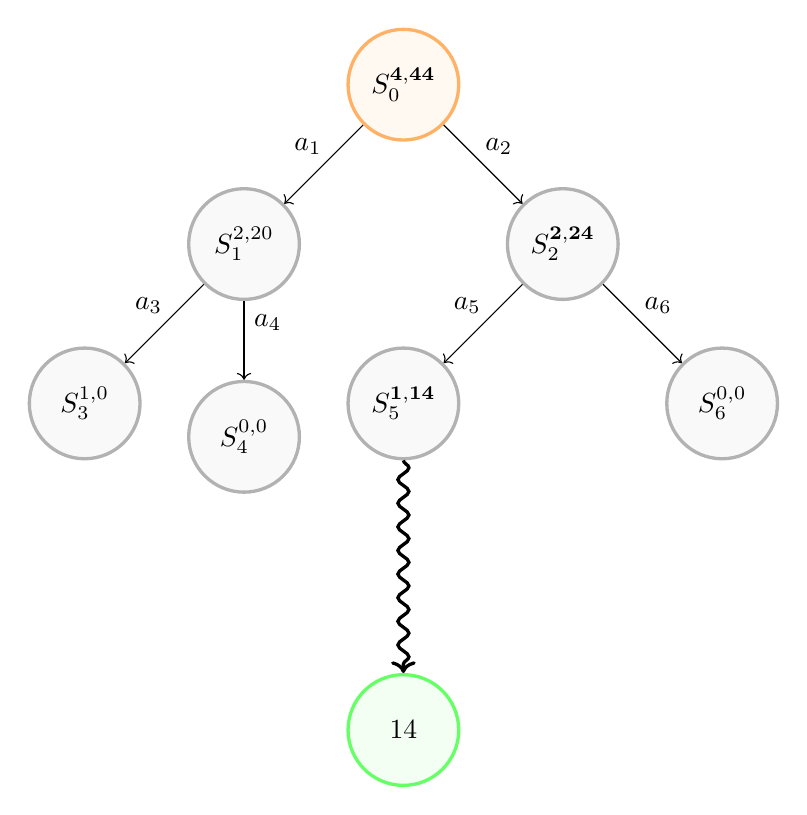
\begin{tikzpicture}[
            root_node/.style={circle, draw=orange!60, fill=orange!5, very thick, minimum size=40},
            visited_node/.style={circle, draw=green!60, fill=green!5, very thick, minimum size=40},
            unvisited_node/.style={circle, draw=gray!60, fill=gray!5, very thick, minimum size=40},
            target_node/.style={circle, draw=green!60, fill=green!5, very thick, minimum size=40},
        ]

        \node[root_node](Root){$S^{\mathbf{4,44}}_0$};
        \node[unvisited_node, below left=of Root](S1){$S^{2,20}_1$};
        \node[unvisited_node, below right=of Root](S2){$S^{\mathbf{2},\mathbf{24}}_2$};
        \node[unvisited_node, below left=of S1](S3){$S^{1,0}_3$};
        \node[unvisited_node, below=of S1](S4){$S^{0,0}_4$};
        \node[unvisited_node, below left=of S2](S5){$S^{\mathbf{1},\mathbf{14}}_5$};
        \node[unvisited_node, below right=of S2](S6){$S^{0,0}_6$};


        \node[target_node, below=of S5, yshift=-1.7cm](Target){14};


        \draw[->] (Root) -- (S1) node[midway, above, xshift=-2mm] {$a_1$};
        \draw[->] (Root) -- (S2) node[midway, above, xshift=2mm] {$a_2$};
        \draw[->] (S1) -- (S3)   node[midway, above, xshift=-2mm] {$a_3$};
        \draw[->] (S1) -- (S4)   node[midway, above, xshift=3mm] {$a_4$};
        \draw[->] (S2) -- (S5) node[midway, above, xshift=-2mm] {$a_5$};
        \draw[->] (S2) -- (S6) node[midway, above, xshift=2mm] {$a_6$};

        \draw[->, very thick, decorate, decoration={snake, amplitude=.7mm, segment length=3mm}] (S5) -- (Target);




    \end{tikzpicture}
    }
    \caption{Selection - Simulation - Backpropagation - $I_{t4}$}
    \label{fig:Selection - Simulation - Backpropagation - I4}
\end{figure}

The MCTS algorithm can either be stopped because the player is running out of time or because the player has no more available actions in the game. For instance, if they were to stop at this stage of the algorithm, the best action to undertake is $a_2$ because it has the higher average value: $\bar{V_1}=\frac{20}{2} \le \bar{V_2}=\frac{24}{2}$.

\subsection{The different parameters in the MCTS}
\label{sub:selection_policies_litterature}

As outlined in the previous example, node's selection is crucial in the MCTS process and can significantly influence the performance of the algorithm.
The selection function traditionally used is the Upper Confidence Bound 1 (UCB). However, there are a lot of different MCTS' selection functions as mentioned in this survey \cite{different_selection_policies}. Most of the selection function, are based on the upper confidence bound principle, which balances the dual aspect of exploration and exploitation in the tree search.

The UCB and its variants, the UCB1-Tuned, are defined as follow:

\begin{equation}
    UCB = \overline{X}_i + C_p \sqrt{\frac{2 \ln N}{n_i}}
    \label{eq:UCB}
\end{equation}

\begin{equation}
    UCB\text{-Tuned} = \overline{X}_i + \sqrt{\frac{\ln N}{n_i} \min\left(\frac{1}{4}, \mathrm{Var}(X_i) + \sqrt{\frac{2 \ln N}{n_i}}\right)}
    \label{eq:UCB1T}
\end{equation}

Where:
\begin{itemize}
    \item \( \overline{X}_i \): Average reward of node \( i \).
    \item \( N \): Total number of visits to the root node.
    \item \( n_i \): Number of visits to node \( i \).
    \item \( C_p \): Exploration parameter.
    \item \( \mathrm{Var}(X_i) \): Variance of the rewards at node \( i \), representing the variability of the rewards.
\end{itemize}

The UCB balances its exploration with the coefficient $C_p$, empirically $C_p=\sqrt2$. The term \( C_p \sqrt{\frac{2 \ln N}{n_i}} \) adds a confidence interval to the average reward, which encourages exploring less-visited nodes when $C_p>0$. When $C_p=0$, the tree search explores less but exploits more of the known part that seems promising for the problem in the tree.
The UCB1-Tuned balances its exploration with \( \min\left(\frac{1}{4}, \mathrm{Var}(X_i) + \sqrt{\frac{2 \ln N}{n_i}}\right) \), making the UCB1-Tuned more adaptable to environments with varying reward distributions. The $C_p$ coefficient can also be considered in the UCB1-Tuned's formula. Hence in stochastic environments the UCB1-Tuned is more likely to have a better overall performance.

Other selection policies, such as the Beta policy or Single Player MCTS \cite{different_selection_policies}, also play significant roles in various applications of the Monte Carlo Tree Search. However, these policies will not be the focus of this study due to their probabilistic nature, which does not align well with our specific problem context.


\subsection{Parallelisation}
\label{sub:parralelisation}

In computer science, parallelisation is a technique that divides a number of tasks into sub-tasks that can be both, independently and simultaneously run on mutiple cores of a computer.
Due to the nature of the MCTS and its four phases, this algorithm is a good candidate for parallelisation.

For instance, after selecting a node to explore, rather than conducting a single simulation based on the one simulation policy, you can either run simulations using multiple different simulation policies and select the best outcome, or perform multiple simulations using the same policy (if it is stochastic). 
Then, going back to the fourth iteration of our example in Figure \ref{fig:Selection - Simulation - Backpropagation - I4}, if we parallelise simulations on three cores then instead of having $\mathcal{R}(S^{0,0}_{5})=14$ you have a list of simulation results $\mathcal{R}(S^{0,0}_{5})=(\mathcal{R}_1(S^{0,0}_{5}),\mathcal{R}_2(S^{0,0}_{5}),\mathcal{R}_3(S^{0,0}_{5}))=(13,14,25)$ and one decision policy could be to pick the maximum of this simulation, hence $\max(\mathcal{R}(S^{0,0}_{5}))=\mathcal{R}_3(S^{0,0}_{5})=25$.

\begin{figure}
    \centering
    \scalebox{0.8}{
    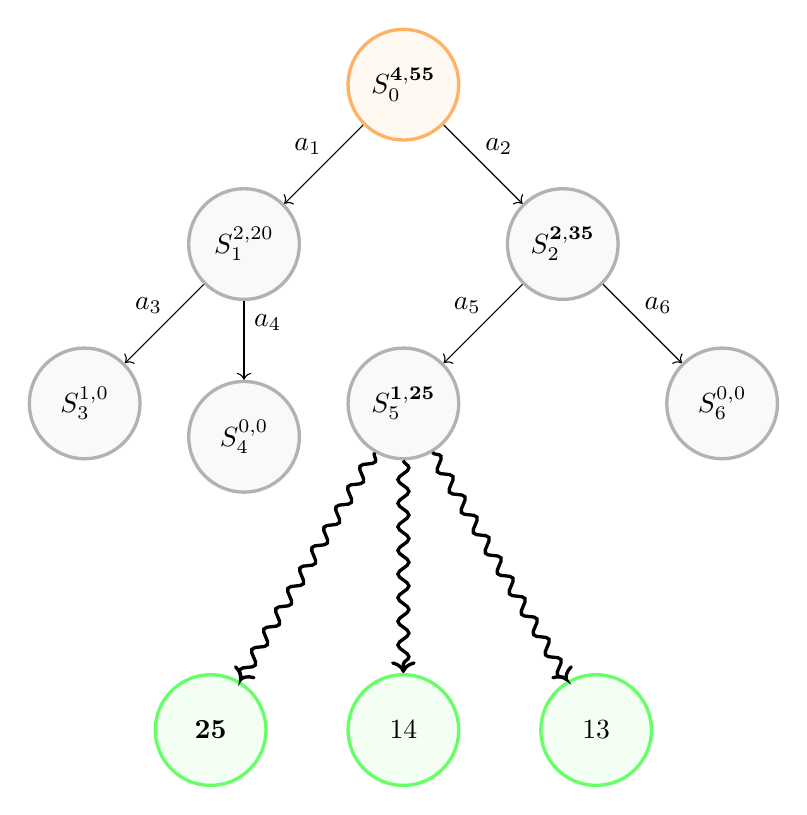
\begin{tikzpicture}[
            root_node/.style={circle, draw=orange!60, fill=orange!5, very thick, minimum size=40},
            visited_node/.style={circle, draw=green!60, fill=green!5, very thick, minimum size=40},
            unvisited_node/.style={circle, draw=gray!60, fill=gray!5, very thick, minimum size=40},
            target_node/.style={circle, draw=green!60, fill=green!5, very thick, minimum size=40},
        ]

        \node[root_node](Root){$S^{\mathbf{4,55}}_0$};
        \node[unvisited_node, below left=of Root](S1){$S^{2,20}_1$};
        \node[unvisited_node, below right=of Root](S2){$S^{\mathbf{2},\mathbf{35}}_2$};
        \node[unvisited_node, below left=of S1](S3){$S^{1,0}_3$};
        \node[unvisited_node, below=of S1](S4){$S^{0,0}_4$};
        \node[unvisited_node, below left=of S2](S5){$S^{\mathbf{1},\mathbf{25}}_5$};
        \node[unvisited_node, below right=of S2](S6){$S^{0,0}_6$};


        \node[target_node, below=of S5, yshift=-1.7cm](Target){14};
        \node[target_node, right=of Target](Target2){13};
        \node[target_node, left=of Target](Target3){$\mathbf{25}$};

        \draw[->] (Root) -- (S1) node[midway, above, xshift=-2mm] {$a_1$};
        \draw[->] (Root) -- (S2) node[midway, above, xshift=2mm] {$a_2$};
        \draw[->] (S1) -- (S3)   node[midway, above, xshift=-2mm] {$a_3$};
        \draw[->] (S1) -- (S4)   node[midway, above, xshift=3mm] {$a_4$};
        \draw[->] (S2) -- (S5) node[midway, above, xshift=-2mm] {$a_5$};
        \draw[->] (S2) -- (S6) node[midway, above, xshift=2mm] {$a_6$};

        \draw[->, very thick, decorate, decoration={snake, amplitude=.7mm, segment length=3mm}] (S5) -- (Target);
        \draw[->, very thick, decorate, decoration={snake, amplitude=.7mm, segment length=3mm}] (S5) -- (Target2);
        \draw[->, very thick, decorate, decoration={snake, amplitude=.7mm, segment length=3mm}] (S5) -- (Target3);

    \end{tikzpicture}
    }
    \caption{Example of parrelisation- $I_{t4}$}
    \label{fig:Selection - Simulation - Backpropagation - I4 - P}
\end{figure}

Multiple parallelisation can be applied in the MCTS. For instance, the multi-tree MCTS aims to build parallelised tree from the root node or the leaf parallelisation where multiple simulations are executed at the same time to get better estimates of the node's value (what is done on Figure \ref{fig:Selection - Simulation - Backpropagation - I4 - P}). However, too many modifications of the MCTS can be unproductive and lead to worst results \cite{different_selection_policies}.

\tikzset{class/.style={rectangle, draw=green!60, fill=green!5, very thick, minimum size=20},
    method/.style={rectangle, draw=yellow!60, fill=yellow!5, very thick, minimum size=20},
    attributes/.style={rectangle, draw=blue!60, fill=blue!5, very thick, minimum size=20},
    instance/.style={rectangle, draw=orange!60, fill=orange!5, very thick, minimum size=20}
}

\section{Monte Carlo Tree Search implementation}
\subsection{General flow}

The flow of the Monte Carlo Tree Search algorithm is summarised in Figure \ref{fig:Flow MCTS}.

\begin{figure}
    \centering
    \scalebox{0.7}{
    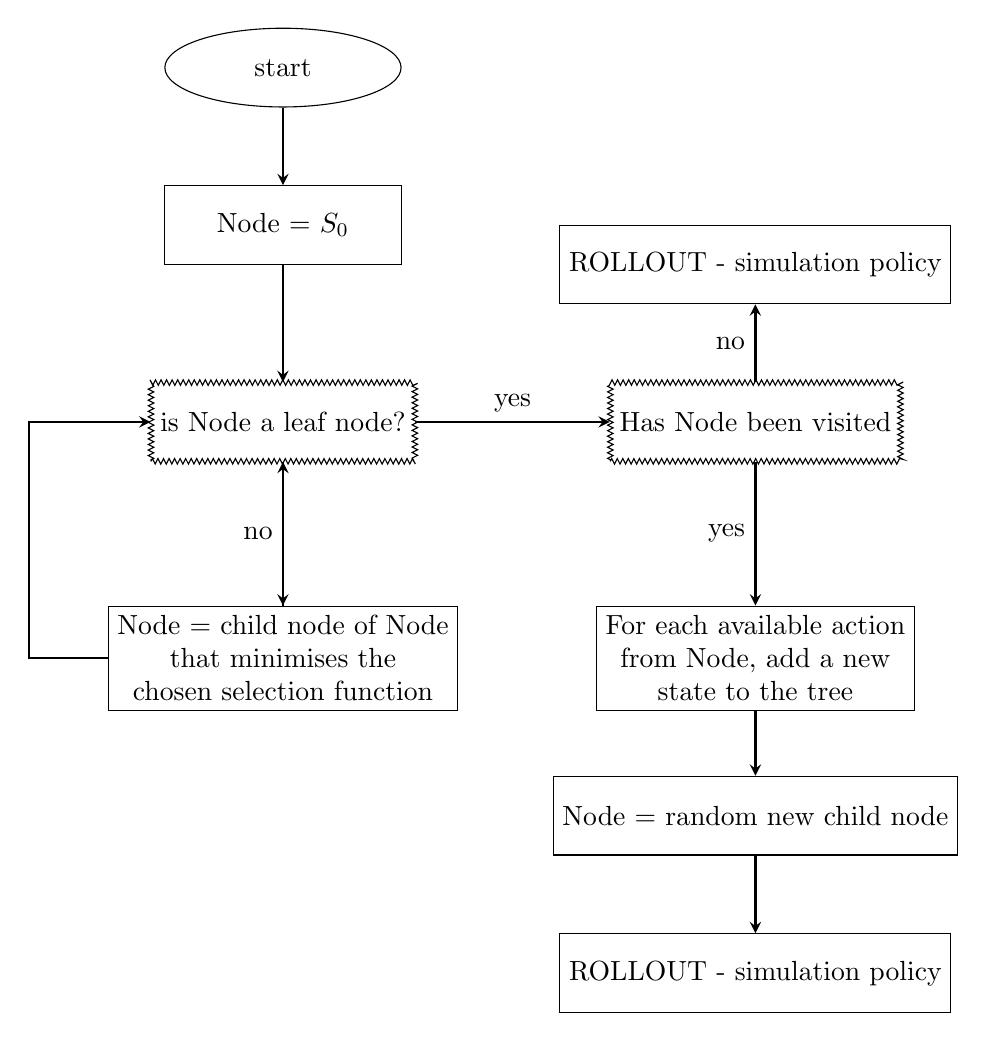
\begin{tikzpicture}[
            startstop/.style={ellipse, minimum width=3cm, minimum height=1cm, text centered, draw=black},
            process/.style={rectangle, minimum width=3cm, minimum height=1cm, text centered, draw=black},
            decision/.style={rectangle, minimum width=3cm, minimum height=1cm, text centered, draw=black, decorate, decoration={zigzag,segment length=2,amplitude=1}},
            arrow/.style={thick,->,>=stealth},
            node distance=2cm
        ]

        \node (start) [startstop] {start};
        \node (current) [process, below of=start] {Node = $S_0$};
        \node (decision1) [decision, below of=current, yshift=-0.5cm] {is Node a leaf node?};
        \node (ucb1) [process, below of=decision1, yshift=-1cm, align=center] {Node = child node of Node \\ that minimises the \\ chosen selection function};
        \node (decision2) [decision, right of=decision1, xshift=4cm] {Has Node been visited};
        \node (expand) [process, below of=decision2, yshift=-1cm, align=center] {For each available action\\ from Node, add a new \\ state to the tree};
        \node (firstChild) [process, below of=expand] {Node = random new child node};
        \node (rollout1) [process, below of=firstChild] {ROLLOUT - simulation policy};
        \node (rollout2) [process, above of=decision2] {ROLLOUT - simulation policy};

        \draw [arrow] (start) -- (current);
        \draw [arrow] (current) -- (decision1);
        \draw [arrow] (decision1) -- node[anchor=east] {no} (ucb1);
        \draw [arrow] (ucb1) -- (decision1);
        \draw [arrow] (decision1) -- node[anchor=south] {yes} (decision2);
        \draw [arrow] (decision2) -- node[anchor=east] {yes} (expand);
        \draw [arrow] (decision2) -- node[anchor=east] {no} (rollout2);
        \draw [arrow] (expand) -- (firstChild);
        \draw [arrow] (ucb1.west) -- ++(-1,0) |- (decision1.west);
        \draw [arrow] (firstChild) -- (rollout1);

    \end{tikzpicture}
    }
    \caption{Flow MCTS}
    \label{fig:Flow MCTS}
\end{figure}

For every iteration of this algorithm, there are four different phases:

\begin{enumerate}
    \item \textbf{Selection:} Starting from the root node (the starting airport $S_{i0}$ for $I_{i}$), select successive child nodes (airports that are in unvisited areas) until a leaf node (the airport in the initial area, not necessarily the starting airport) is reached. Use the chosen Selection function to evaluate which node is the most promising. In the illustrative example, the UCB1 (also called UCB) function was used for the selection function. Furthermore, the problem's goal was to maximise the objective function, hence the nodes with the highest UCB1 value was selected. However, in Kiwi's minimisation problem,  nodes are evaluated based on the lowest value of the selection function.

    \item \textbf{Expansion:} If the selected node is not a terminal node, expand the tree by adding all possible child nodes.

    \item \textbf{Simulation:} From the newly added node, perform a simulation (based on the simulation policy) until a feasible terminal node is reached.

    \item \textbf{Backpropagation:} Update the values of the nodes along the path from the newly added node to the root based on the result of the simulation.

          \begin{equation}
              \mathcal{B}(S^{n_i,t_i}_i) = S^{n_i+1,t_i+\mathcal{R}(S^{n_i,t_i}_i)}_i
          \end{equation}

          where $\mathcal{R}(S^{n_i,t_i}_i)$ is the cost of the solution found after performing a simulation from node $S^{n_i,t_i}_i$.
\end{enumerate}

\subsubsection{Data Preprocessing}

To implement our MCTS' solution, the first thing to create is a DataPreprocessing \tikz[baseline=(class.base)]{\node[class] (class) {class};} to prepare the given instance to the problem at hand. 
Kiwi's challenge is solved using Python 3.10 on VS Code 1.92.2. Our Python code is structured using object-oriented programming following CamelCase's convention \cite{camel_case}. This DataPreprocessing class is represented on Figure \ref{fig:data_preprocessing_class}. The input is an \tikz[baseline=(instance.base)]{\node[instance] (instance) {instance};} $I_i$.

\begin{figure}
    \centering
    \scalebox{0.7}{
    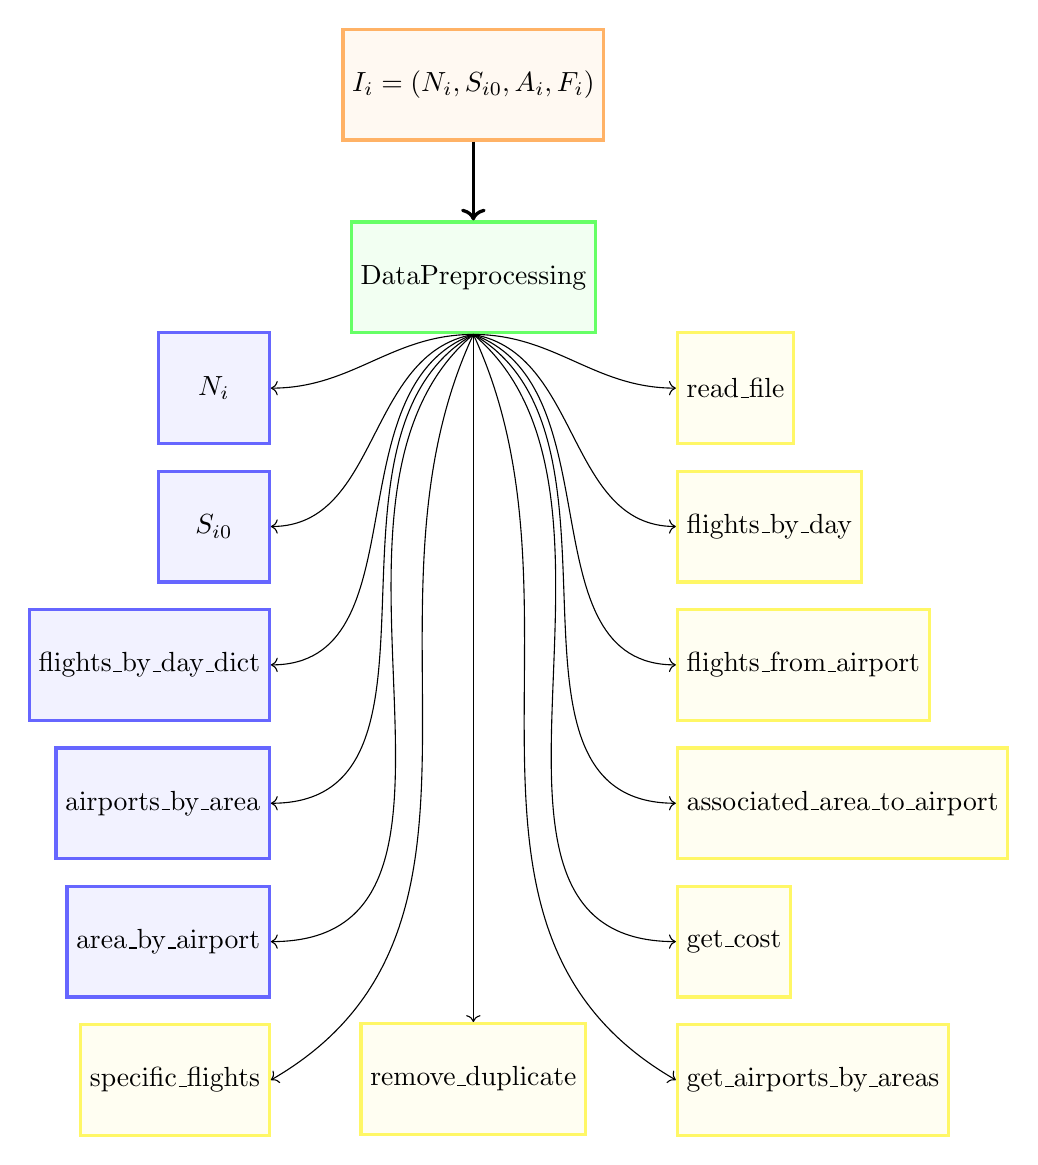
\begin{tikzpicture}[
            class/.style={rectangle, draw=green!60, fill=green!5, very thick, minimum size=40},
            methods/.style={rectangle, draw=yellow!60, fill=yellow!5, very thick, minimum size=40},
            attributes/.style={rectangle, draw=blue!60, fill=blue!5, very thick, minimum size=40},
            instance/.style={rectangle, draw=orange!60, fill=orange!5, very thick, minimum size=40}
        ]

        %Nodes  
        \node[instance]          (Instance){$I_i = (N_i, S_{i0}, A_{i}, F_{i})$};
        \node[class]             (Class)[below=of Instance]{DataPreprocessing};

        \node[attributes, left=of  Class , yshift=-40] (Attr1) {$N_i$};
        \node[attributes, left=of  Class , yshift=-90] (Attr2) {$S_{i0}$};
        \node[attributes, left=of  Class , yshift=-140] (Attr3) {flights\_by\_day\_dict};
        \node[attributes, left=of  Class, yshift=-190] (Attr4) {airports\_by\_area};
        \node[attributes, left=of  Class, yshift=-240] (Attr5) {area\_by\_airport};
        %\node[methods, left=of Class, yshift=-290, align=center] (Meth10) {flights\_from\_airport\_at\_a\_\\specific\_day\_with\_previous\_areas};
        \node[methods, left=of Class, yshift=-290, align=center] (Meth10) {specific\_flights};


        \node[methods, right=of  Class, yshift=-40] (Meth1) {read\_file};
        \node[methods, right=of  Class, yshift=-90] (Meth2) {flights\_by\_day};
        \node[methods, right=of  Class, yshift=-140] (Meth3) {flights\_from\_airport};
        \node[methods, right=of  Class, yshift=-190] (Meth4) {associated\_area\_to\_airport};
        \node[methods, right=of  Class, yshift=-240] (Meth5) {get\_cost};
        \node[methods, right=of  Class, yshift=-290] (Meth6) {get\_airports\_by\_areas};
        \node[methods, below=of  Class, yshift=-220] (Meth7) {remove\_duplicate};

        %Lines
        \draw[->, very thick] (Instance.south)  to node[midway, right] {} (Class.north);

        \draw[->] (Class.south) to[out=180, in=0] (Attr1.east);
        \draw[->] (Class.south) to[out=190, in=0] (Attr2.east);
        \draw[->] (Class.south) to[out=200, in=0] (Attr3.east);
        \draw[->] (Class.south) to[out=210, in=0] (Attr4.east);
        \draw[->] (Class.south) to[out=220, in=0] (Attr5.east);

        % Arrows from Class to Methods (right side)
        \draw[->] (Class.south) to[out=0, in=180] (Meth1.west);
        \draw[->] (Class.south) to[out=350, in=180] (Meth2.west);
        \draw[->] (Class.south) to[out=340, in=180] (Meth3.west);
        \draw[->] (Class.south) to[out=330, in=180] (Meth4.west);
        \draw[->] (Class.south) to[out=320, in=180] (Meth5.west);

        \draw[->] (Class.south) to[out=-115, in=30] (Meth10.east);
        \draw[->] (Class.south) to[out=-65, in=150] (Meth6.west);
        \draw[->] (Class.south) to[out=-90, in=90] (Meth7.north);
    \end{tikzpicture}
    }
    \caption{Explanation of the data preprocessing class}
    \label{fig:data_preprocessing_class}
\end{figure}

Different useful \tikz[baseline=(methods.base)]{\node[method] (methods) {methods};} are implemented within this class to compute and manage various attributes required for the problem at hand. These methods are designed to prepare and structure the data, making it easier to use in subsequent phases of the algorithm. 
For example, the remove\_duplicate method ensures that only the cheapest flight connections are considered between two airports if multiple flight connections exist at different prices, on the same day. 
Other methods, such as flights\_by\_day\_dict and get\_airports\_by\_areas organise the data. The first method regroups all the flights by their respective days, creating a dictionary where each key represents a day and its corresponding value is a list of available flights. The second method regroups all the airports present in the different areas.

Finally, other methods, such as specific\_flights, will be useful for developing the MCTS' algorithm. These give all the possible flight connections from a specific airport on a given day, taking into account the areas visited, so that all possible actions can be obtained from a node.

Given that Python is relatively slower than other programming languages, in terms of computation, dictionaries are used where possible. Dictionaries allow for efficient data retrieval based on a key, with an average time complexity of $\mathcal{O}(1)$. This choice improves the performance of the data preprocessing step, enabling the algorithm to run more efficiently despite Python’s inherent limitations.

\subsubsection{Node}
\label{subsub:node}
\begin{figure}[h]
    \centering
    \scalebox{0.8}{
    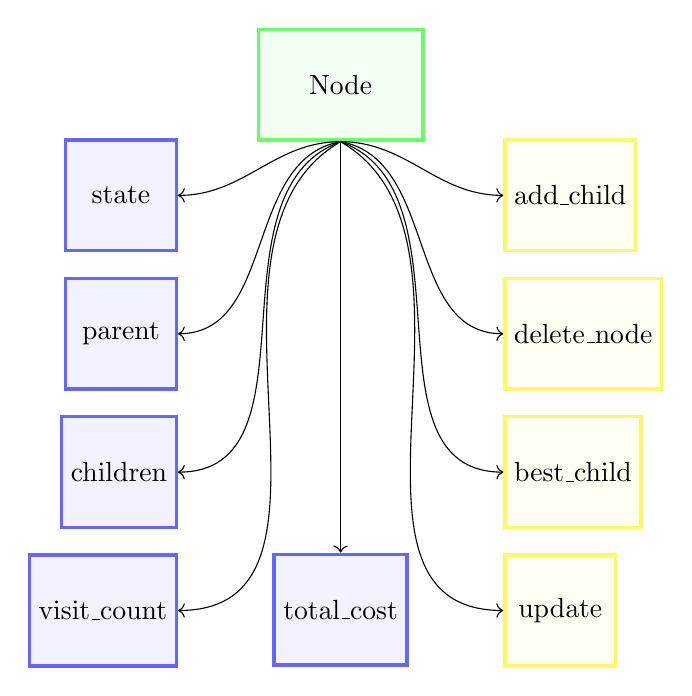
\begin{tikzpicture}[
            class/.style={rectangle, draw=green!60, fill=green!5, very thick, minimum size=40},
            methods/.style={rectangle, draw=yellow!60, fill=yellow!5, very thick, minimum size=40},
            attributes/.style={rectangle, draw=blue!60, fill=blue!5, very thick, minimum size=40},
            instance/.style={rectangle, draw=orange!60, fill=orange!5, very thick, minimum size=40}
        ]

        \node[class]             (Class){\phantom{-----}Node\phantom{-----}};

        \node[attributes, left=of  Class , yshift=-40] (Attr1) {state};
        \node[attributes, left=of  Class , yshift=-90] (Attr2) {parent};
        \node[attributes, left=of  Class , yshift=-140] (Attr3) {children};
        \node[attributes, left=of  Class, yshift=-190] (Attr4) {visit\_count};

        \node[methods, right=of  Class, yshift=-40] (Meth1) {add\_child};
        \node[methods, right=of  Class, yshift=-90] (Meth2) {delete\_node};
        \node[methods, right=of  Class, yshift=-140] (Meth3) {best\_child};
        \node[methods, right=of  Class, yshift=-190] (Meth4) {update};

        \node[attributes, below=of  Class, yshift=-120] (Meth5) {total\_cost};


        \draw[->] (Class.south) to[out=180, in=0] (Attr1.east);
        \draw[->] (Class.south) to[out=190, in=0] (Attr2.east);
        \draw[->] (Class.south) to[out=200, in=0] (Attr3.east);
        \draw[->] (Class.south) to[out=210, in=0] (Attr4.east);

        \draw[->] (Class.south) to[out=0, in=180] (Meth1.west);
        \draw[->] (Class.south) to[out=350, in=180] (Meth2.west);
        \draw[->] (Class.south) to[out=340, in=180] (Meth3.west);
        \draw[->] (Class.south) to[out=330, in=180] (Meth4.west);

        \draw[->] (Class.south) to[out=-90, in=90] (Meth5.north);

    \end{tikzpicture}
    }
    \caption{Explanation of the Node class}
    \label{fig:node_class}
\end{figure}

A Node structure is used in the algorithm, hence the implementation of a Node class. 
Each Node has a reference to a parent node (unless it is the root node) and may have one or more child nodes (unless it is a leaf node). These relationships form a tree structure where each node can expand into potential future states, guiding the search process. 
The visit\_count tracks the number of times a node has been visited during the MCTS process. This is crucial for evaluating the node's importance and for calculating the score of the node with the selection function. 
The state is a dictionary that contains the node's current information:
\begin{itemize}
    \item current\_airport: The airport where the traveller is  at this node.
    \item current\_day: The day of the trip at this node.
    \item remaining\_zones: The zones that still need to be visited to complete the journey.
    \item visited\_zones: The zones that have already been visited to ensure that all zones are visited exactly once during the trip.
    \item total\_cost: It represents the accumulated cost of the current solution path leading to this node.
\end{itemize}

Additionally, to manage the expansion of child nodes, the add\_child method is defined. 
This method generates new nodes based on the possible actions available from the current node. These new nodes represent the next possible states in the traveller’s journey, allowing the search tree to expand and explore different travel routes. 
Finally, the delete\_node method can be used to delete a node from the list of its parent's children. 



\section{The different policies}

In the previous section, we outlined the general flow of the MCTS algorithm, focusing on two cores classes, DataPreprocessing and Node, that are central in MCTS' implementation.

In Section \ref{sub:selection_policies_litterature}, we explored the various selection policies that guide the decision-making process within the MCTS
Although there is a limited literature review, we decided to parameterise not only the selection policy but also the simulation and expansion policies.

\subsection{Simulation policies}
\label{sub:simulation_policies}
When a simulation is run from a given node in the tree, the goal is to find a feasible combination of airports that could be a solution to our problem.
From this node chosen for the simulation, we obtain the current state (defined in section \ref{subsub:node}). The remaining actions must then be chosen to find a simulated solution based on the simulation policy.

Below is the definition of the three distinct simulation policies:

\begin{itemize}
    \item Random policy: This policy selects a random action from the set of available actions, introducing variability and exploration in the simulation process.
    \item Greedy policy: This policy selects the action that corresponds to the cheapest available flight connection, thus prioritising cost minimisation at each step.

    \item Tolerance policy (with coefficient $c$):
          This policy selects an action randomly from a subset of actions that are within a certain tolerance level of the minimum cost action. The tolerance level is defined by a coefficient $c$. The tolerance policy is defined as follows:
          \begin{itemize}
              \item Identify the cheapest flight connection among the available actions $c_{min}$.
              \item Filter the actions to include only those with a cost less or equal than $c_{min}(1+c) $.
              \item Randomly select an action from this filtered set.
          \end{itemize}
          This policy introduces a more balanced approach than the random and greedy policies, balancing between optimal moves and random ones.
\end{itemize}



\subsection{Expansion policies}
\label{sub:expansion_policies}
When expanding a node, it is theoretically possible to expand all available child nodes i.e., add to the tree all the possible flight connections from this airport (that are in the available actions based on the visited areas). However, in practice, this can be computationally expensive and time-consuming, particularly in problems with a large number of possible actions. To address this, heuristic approaches often involve compromises that enhance the efficiency of the search process by selectively expanding certain nodes rather than all possible ones.

Firstly, we defined \texttt{number\_of\_children}, a parameter of our MCTS algorithm which regulates the maximum number of children that can be expanded from any given node. This limitation controls the size of the search tree, as expanding too many children for every selected node could make the algorithm computationally exhaustive. In our implementation we defined two expansion policies:

\begin{itemize}
    \item \textbf{Top-K policy}: This policy expands the nodes corresponding to the cheapest flight connections available. Specifically, it sorts all possible actions based on their associated costs and selects the top \(k\) actions with the lowest costs, where \(k\) is regulated by \texttt{number\_of\_children}. This approach ensures that only the most promising actions, in terms of cost efficiency, are considered during expansion. This policy narrows down the search space but can increase the chance to reach a leaf node.
    \item \textbf{Ratio policy}: This policy takes a more balanced approach by combining the selection of the best actions with a degree of randomness. First, it calculates the number of top actions to select based on a predefined ratio, \(c \in [0,1]\), which reflects the proportion of Top-K Actions within the allowed \texttt{number\_of\_children}. After selecting these best actions, the policy randomly selects $(1-c)*number\_of\_children$ actions from the remaining pool to reach the desired number of children. This policy is designed to explore a broader range of potential solutions while still prioritising cost-effective options.
\end{itemize}

\subsection{Notations}
\label{sub:notations}

After defining the different parameters of the MCTS, a MCTS function can be defined as follow:

\begin{center}
    \centering
    $\begin{array}{cc}
            \mathcal{MCTS} : S_p(C_p), E_p(c), R_p, N_c & \mapsto \\ ~~~~~~~~~~ \mathcal{MCTS}(S_p(C_p), E_p(c), R_p, N_c) \\
        \end{array}$
\end{center}

where:
\begin{itemize}
    \item $S_p(C_p)$: Selection policy (UCB or UCB1-T) with exploration parameter $C_p$ (defined in Section \ref{sub:selection_policies_litterature}).
    \item $E_p(c)$: Expansion policy (Top-k or Ratio (with ratio $c$)) (defined in Section \ref{sub:expansion_policies}).
    \item $R_p$: Rollout/simulation policy (random, tolerance, or greedy) (defined in Section \ref{sub:simulation_policies}).
    \item $N_c$: Maximum number of children added during node expansion.
\end{itemize}

\subsection{Pseudo-code}
In this section, the implementation of the algorithm in practice is explored by examining the different functions of our MCTS class. The search function of the MCTS is defined:

\begin{algorithm}[H]
    \caption{Search\_Function}
    \label{alg:MCTS}
    \begin{algorithmic}[1]
        \STATE Initialise Root\_Node with Initial\_State
        \WHILE{Tree is not fully explored}
        \STATE $Node \leftarrow \text{Select}(Root\_Node)$
        \IF{$Node$ is not fully expanded}
        \STATE $Node \leftarrow \text{Expand}(Node)$
        \ENDIF
        \STATE $Cost \leftarrow \text{Simulate}(Node)$
        \STATE \text{Backpropagate}($Node$, $Cost$)
        \ENDWHILE
        \RETURN $Best\_Leaf\_Node$
    \end{algorithmic}
\end{algorithm}

The \texttt{Search} function represents the general flow of the algorithm as mentioned on Figure \ref{fig:Flow MCTS}.

The \texttt{Select} function (Algorithm \ref{alg:SelectFunction}), which selects the node to visit, returns two arguments: a boolean and a node. The boolean indicates to the expansion function whether expansion is necessary (True means no expansion needed, False means expansion needed).

\begin{algorithm}[H]
    \caption{Select\_Function}
    \label{alg:SelectFunction}
    \begin{algorithmic}[1]
        \STATE \textbf{Input:} $Node$
        \STATE $Current \leftarrow Node$
        \WHILE{$Current.Children$ is not empty}
        \IF{Current is not fully expanded}
        \STATE $UnvisitedChildren \leftarrow$ \\ $\text{Children with } VisitCount = 0$
        \IF{$UnvisitedChildren$ is not empty}
        \STATE $SelectedChild \leftarrow$ \\ $\text{Randomly select from } UnvisitedChildren$
        \RETURN $True, SelectedChild$
        \ENDIF
        \ELSE
        \STATE $Current \leftarrow \text{BestChild}(Current)$
        \ENDIF
        \ENDWHILE
        \IF{$Current.Children$ is empty \textbf{and} $Current.State["current\_day"]==N_{Areas}$}
        \RETURN $False, Current$
        \ELSIF{$Current.Children$ is empty \textbf{and} $Current.State["current\_day"]<>N_{Areas}$}
        \RETURN $False, Current$
        \ELSIF{$Current.State["current\_day"]==N_{Areas} + 1$}
        \RETURN $True, Current$
        \ENDIF
    \end{algorithmic}
\end{algorithm}

There are special cases to handle, when one approaches the final solution because one has to communicate the right information to the \texttt{Expand Node} function.

After simulating, the backpropagation function updates the node's attributes. The new node becomes the parent of this node, and so on until \texttt{Node} is \texttt{None}, i.e., all the information is backpropagated up to the root node.

\begin{algorithm}
    \caption{Backpropagate\_Function}
    \label{alg:Backpropagate}
    \begin{algorithmic}[1]
        \WHILE{$Node$ is not $None$}
        \STATE $Node.Update(Cost)$
        \STATE $Node \leftarrow Node.Parent$
        \ENDWHILE
    \end{algorithmic}
\end{algorithm}

The transition function modifies the states of a node by updating the current airport, the visited zones, remaining zones, etc.

\begin{algorithm}
    \caption{Transition\_Function}
    \label{alg:TransitionFunction}
    \begin{algorithmic}[1]
        \STATE $New\_State \leftarrow \text{Copy of } State$
        \STATE $New\_State.Current\_Day \leftarrow State.Current\_Day + 1$
        \STATE $New\_State.Current\_Airport \leftarrow Action[0]$
        \STATE $New\_State.Total\_Cost \leftarrow State.Total\_Cost + Action[1]$
        \STATE \text{Update}($New\_State.Path$, $New\_State.Current\_Airport$)
        \STATE \text{Remove\_Visited}($New\_State.Remaining\_Zones$, $New\_State.Current\_Airport$)
        \STATE \text{Add\_Visited}($New\_State.Visited\_Zones$, $New\_State.Current\_Airport$)
        \RETURN $New\_State$
    \end{algorithmic}
\end{algorithm}

Finally, the Best Child function, defined in the Node class is based on the selection function UCB and UCB1\_Tuned. They both, compute the score of the visited nodes and pick the one that minimises the selection function.

\begin{algorithm}
    \caption{Best Child}
    \label{alg:Best Child}
    \begin{algorithmic}[1]
        \REQUIRE $Selection\_Function$
        \STATE $Visited\_Children \leftarrow \text{Children with } visitCount > 0$
        \STATE $Choices\_Weights \leftarrow$ 
        \\ $\left[ Selection\_Function(child) \text{ for child in } Visited\_Children \right]$
        \STATE $Best\_Child\_Node \leftarrow$ \\ $\text{Child with minimum } Choices\_Weights$
        \RETURN $Best\_Child\_Node$
    \end{algorithmic}
\end{algorithm}

\section{Test Instances}

We are given a set of 14 instances \( I_{n} = \{I_1, I_2, \ldots, I_{13}, I_{14}\} \). For example, the first few lines of instance \( I_4 \) are:

\begin{center}
    \begin{tabular}{|l|}
    \hline
        \textcolor{gray}{13} \textcolor{blue}{GDN}      \\
        first                                           \\
        \textcolor{orange}{WRO} \textcolor{purple}{DL1} \\
        \textcolor{red}{second}                         \\
        BZG KJ1                                         \\
        third                                           \\
        BXP LB1                                         \\
    \hline
    \end{tabular}
\end{center}

This means that the traveller has to visit \textcolor{gray}{13} different areas, starting at the airport \textcolor{blue}{GDN}, which belongs to the starting area. The list of airports in each area is then provided. For example, the second area is named \textcolor{red}{second} and contains two airports: \textcolor{orange}{WRO} and \textcolor{purple}{DL1}.

After all the information regarding the areas and airports is provided, we then have the flight connections data. In Table \ref{table:Flight connections sample I6}, a few flight connections from instance \( I_6 \) are displayed for illustrative purposes.

\begin{table}
    \centering
    \caption{Flight connections sample for instance $I_6$}
    \begin{tabular}{cccc}
        \toprule
        Departure from & Arrival & Day & Cost \\ %[1ex]
        \midrule
        KKE            & BIL     & 1   & 19   \\
        UAX            & NKE     & 73  & 16   \\
        UXA            & BCT     & 0   & 141  \\
        UXA            & DBD     & 0   & 112  \\
        UXA            & DBD     & 0   & 128  \\
        UXA            & DBD     & 0   & 110  \\
        %[1ex]
        \bottomrule
    \end{tabular}
    \label{table:Flight connections sample I6}
\end{table}

For each instance \( I_i \), we know the available flight connections between two airports on specific days and their associated costs. In some instances, flights may be available on day 0, meaning these connections exist for every day of the journey at the same price. Moreover, there may be multiple flights between the same airports on a specific day, but with varying prices. In such cases, we consider only the most relevant connections, i.e., the flight connection with the lowest fare. For example, in Table \ref{table:Flight connections sample I6}, we only consider the flight from UXA to DBD with the lowest associated cost of 110.

When solving all the instances, Kiwi.com defined time limit constraints based on the nature of the instance. These constraints are summarised in Table \ref{table:Time limit constraints}.

\begin{table}
    \centering
    \caption{Time limits based on the number of areas and airports}
    \begin{tabular}{>{\centering\arraybackslash}p{1cm}|>{\centering\arraybackslash}p{1cm}|>{\centering\arraybackslash}p{1.3cm}|>{\centering\arraybackslash}p{1.1cm}}
        \toprule
        Instance Type & Number of Areas & Number of Airports & Time Limit (s) \\ 
        \midrule
        Small         & $\leq 20$        & $<50$             & 3              \\
        Medium        & $\leq 100$       & $<200$            & 5              \\
        Large         & $>100$           &                   & 15             \\ 
        \bottomrule
    \end{tabular}
    \label{table:Time limit constraints}
\end{table}

All the relevant information about the instances, such as the starting airport, the associated area, the range of airports per area, the number of airports, and the time limit constraints, are defined in Table \ref{table:Instances presentation}.

\begin{table}
    \centering
    \caption{Instances and their respective parameters}
    \resizebox{0.49\textwidth}{!}{ % Resize the table to fit the text width
        \begin{tabular}{>{\centering\arraybackslash}p{0.6cm}
            >{\centering\arraybackslash}p{2.3cm}
            >{\centering\arraybackslash}p{1cm}
            >{\centering\arraybackslash}p{2.1cm}
            >{\centering\arraybackslash}p{1cm}
            >{\centering\arraybackslash}p{1.1cm}}
            \toprule
            Instance & Starting Area - Airport & Number of Areas & Min - Max Airports per Area & Total Airports & Time Limit (s) \\
            \midrule
            $I_1$    & Zona\_0 - AB0        & 10  & 1 - 1 & 10  & 3  \\
            $I_2$    & Area\_0 - EBJ        & 10  & 1 - 2 & 15  & 3  \\
            $I_3$    & Ninth - GDN          & 13  & 1 - 6 & 38  & 3  \\
            $I_4$    & Poland - GDN         & 40  & 1 - 5 & 99  & 5  \\
            $I_5$    & Zone0 - RCF          & 46  & 3 - 3 & 138 & 5  \\
            $I_6$    & Zone0 - VHK          & 96  & 2 - 2 & 192 & 5  \\
            $I_7$    & Abfuidmorz - AHG     & 150 & 1 - 6 & 300 & 15 \\
            $I_8$    & Atrdruwkbz - AEW     & 200 & 1 - 4 & 300 & 15 \\
            $I_9$    & Fcjsqtmccq - GVT     & 250 & 1 - 1 & 250 & 15 \\
            $I_{10}$ & Eqlfrvhlwu - ECB     & 300 & 1 - 1 & 300 & 15 \\
            $I_{11}$ & Pbggaefrjv - LIJ     & 150 & 1 - 4 & 200 & 15 \\
            $I_{12}$ & Unnwaxhnoq - PJE     & 200 & 1 - 4 & 250 & 15 \\
            $I_{13}$ & Hpvkogdfpf - GKU     & 250 & 1 - 3 & 275 & 15 \\
            $I_{14}$ & Jjewssxvsc - IXG     & 300 & 1 - 1 & 300 & 15 \\
            \bottomrule
        \end{tabular}
    }
    \label{table:Instances presentation}
\end{table}


\section{Comprehensive Results}

The primary objective was to implement a new algorithm to find solutions without imposing time constraints. Hence, simulations for every instances have been conducted, testing different combinations of parameters in what is called a grid search. Each combination of parameters was run 10 times to ensure the reliability and consistency of the results.
One challenge, is that the computational budget is limited when using Python. Hence, the size of the grid search for the more complex studied instances is reduced. 

After running the various simulations with the grid search parameters, our results were compared with the best known solutions. A solution was found for $I_1, I_2, I_3, I_4,I_7$ and $I_8$. 

\subsection{Analysis}
\subsubsection{$I_1$, $I_2$, $I_3$ and $I_4$}
For instances $I_1, I_2$ and $I_3$, solutions were found and the various simulations were carried out successfully. Therefore, the influence of the parameters on the $\mathcal{MCTS}$ function and the final solution was investigated.
However, only few parametrisation of the $\mathcal{MCTS}$ allowed finding a solution for $I_4$: the UCB1T selection policy and tolerance or random simulation policy created a tree too large to find solutions in a reasonable time (discussed in the following section).

\subsubsection*{Analysis on $C_p$}
\begin{figure}[!ht]
    \centering
    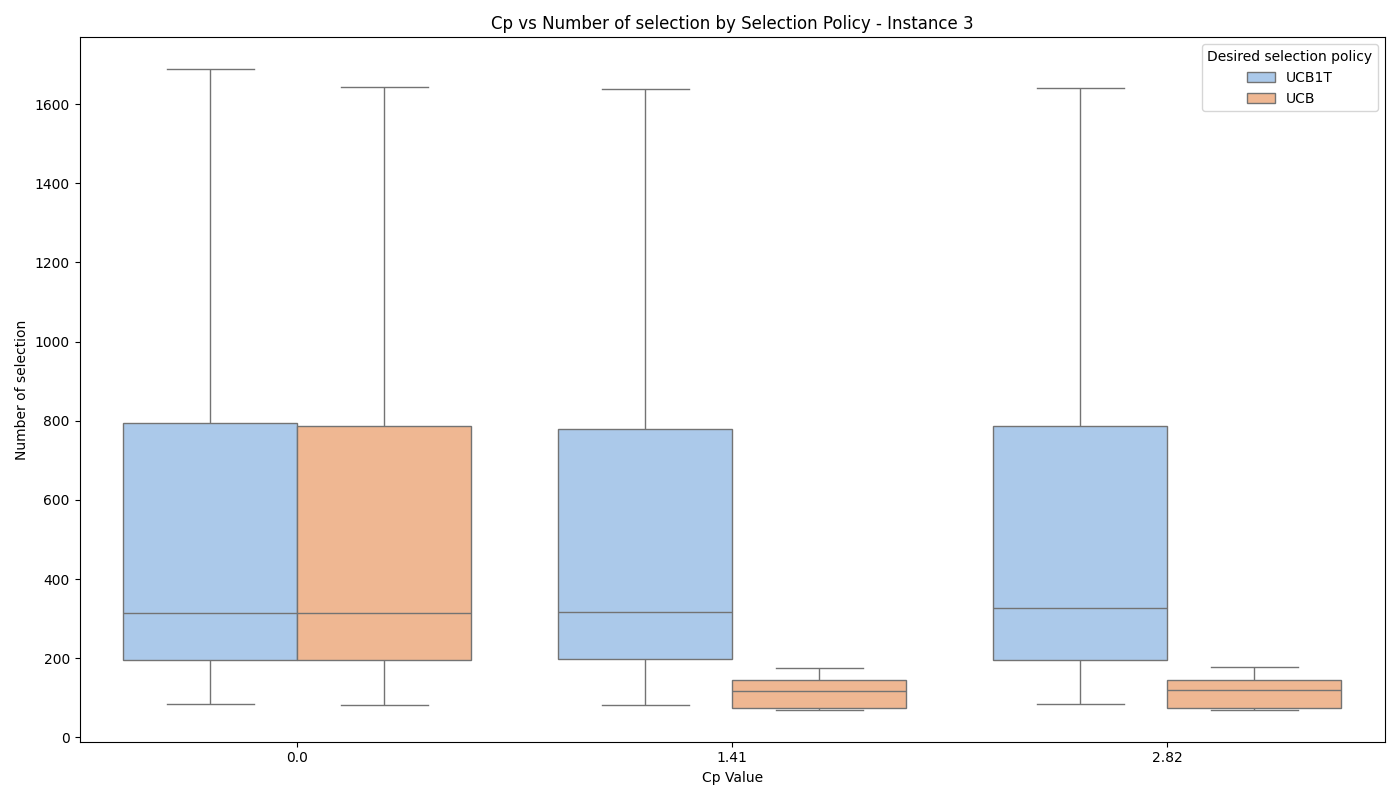
\includegraphics[width=0.42\textwidth]{Figures/3 - cp_vs_selection.png}
    \caption{$C_p$ vs Number of selection}
    \label{fig:cp_vs_selection_3}
\end{figure}

In Figure \ref{fig:cp_vs_selection_3}, the box plots illustrate the relationship between the exploration constant \( C_p \) and the number of selection phases under the UCB and UCB1T selection policies:

\begin{itemize}
    \item \textbf{\( C_p = 0 \) lead to the same performance:}
          When the $C_p=0$, the selection policy of the UCB and the UCB1T are equal, leading to the same decision-making during the MCTS (cf equation \ref{eq:UCB} and \ref{eq:UCB1T}).
    \item \textbf{Higher \( C_p \) values lead to faster convergence for UCB:}
          As \( C_p \) increases from $0.0$ to $2.82$, the median number of selection phases under the UCB policy decreases.

    \item \textbf{UCB1T encourages more exploration:}
          UCB1T consistently results in a higher number of selection phases compared to UCB, especially at higher \( C_p \) values. This is consistent with UCB1T's definition to promote broader exploration before converging.
\end{itemize}

Although a higher exploration parameter $C_p$ may lead to faster convergence under the UCB selection policy, it often results in worse outcomes compared to the UCB1T algorithm, as shown in Figure \ref{fig:cp_vs_cost_3}.
\begin{figure}[!ht]
    \centering
    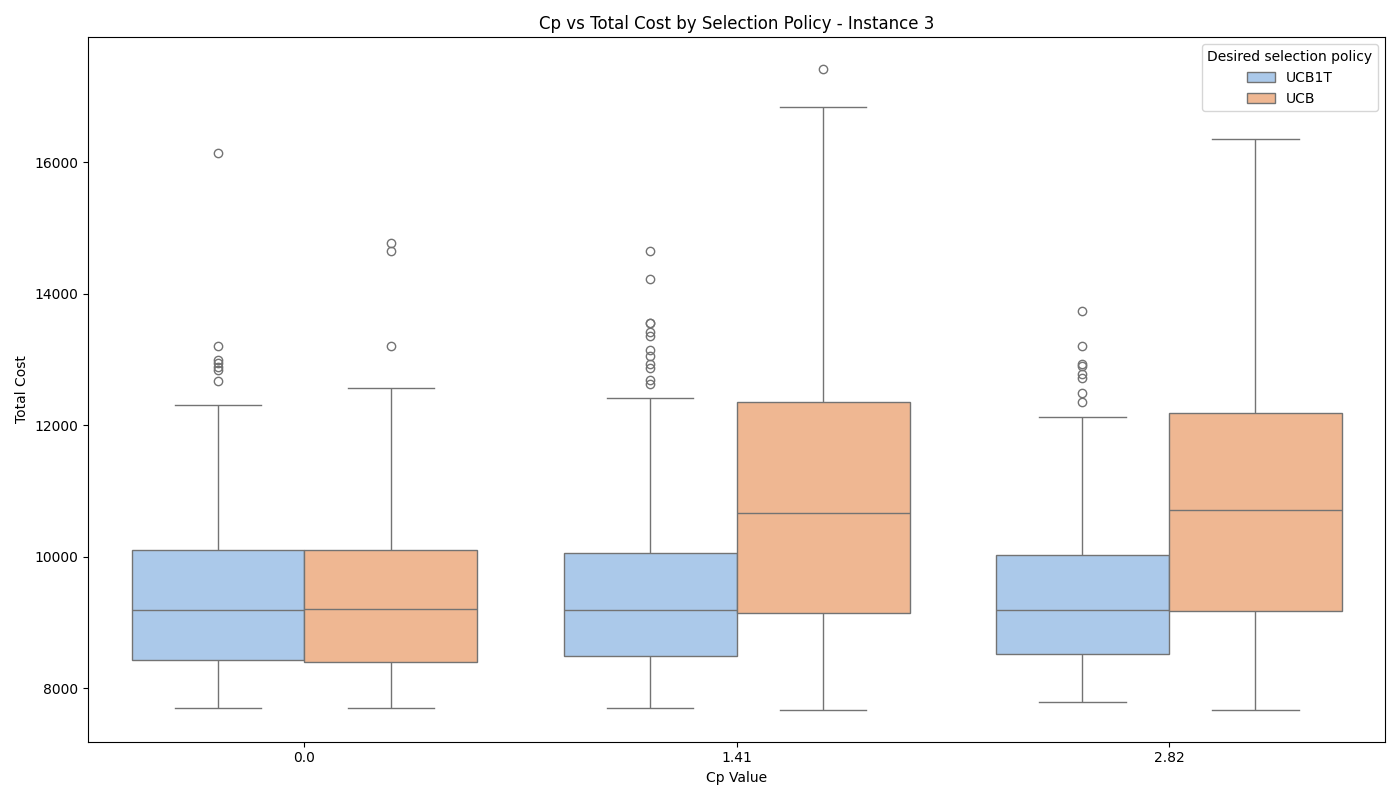
\includegraphics[width=0.42\textwidth]{Figures/3 - cp_vs_cost.png}
    \caption{$C_p$ vs Total cost}
    \label{fig:cp_vs_cost_3}
\end{figure}
While UCB1T may require more time to converge, it generally explores the search tree more effectively, leading to better overall performance. One can notice that $C_p$'s correlation with the UCB1T selection policy for $I_3$ is low.


\subsubsection*{Analysis of expansion ratio $c$}

\begin{figure}[!ht]
    \centering
    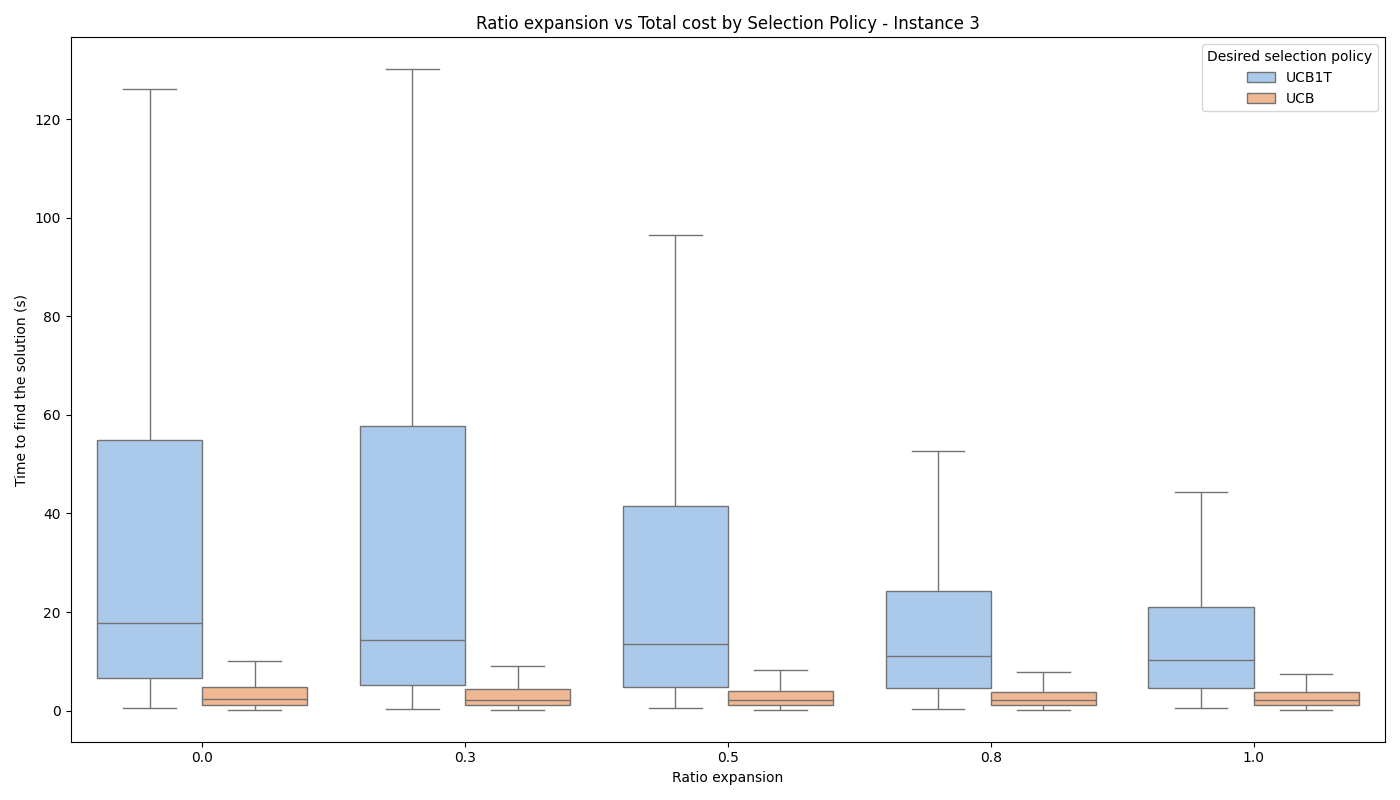
\includegraphics[width=0.42\textwidth]{Figures/3 - ratio_vs_time.png}
    \caption{Ratio expansion vs Time to find the solution}
    \label{fig:Ratio vs Time}
\end{figure}

The box plots show the relationship between ratio expansion (the proportion of expanded child nodes that has the cheapest flight connection over the chosen number of children) and the time to find a solution for the UCB and UCB1T policies:

\begin{itemize}
    \item \textbf{UCB finds solution faster than UCB1T:}
          Across all ratio expansion values, the UCB policy consistently finds solutions more quickly than UCB1T. This suggests that UCB, being less aggressive in exploration, converges on solutions faster.

          %\item \textbf{UCB1T Takes Longer Due to Extensive Exploration:}
          %      UCB1T shows higher and more variable times to find solutions, especially at lower ratio expansions (e.g., $0.0$). This reflects UCB1T's property to explore more than UCB.

    \item \textbf{Higher ratios lead to a faster convergence:}
          For both policies, the time to find a solution generally decreases as the ratio expansion increases, indicating a more efficient search process when expanded nodes are less chosen randomly from the set of available actions. However, in more complex instances, it is crucial to have a ratio $r \in [0.3,0.7]$ to escape potential leaf node.
\end{itemize}

Finally, the UCB policy is more correlated to the expansion ratio than the UCB1T as shown in Figure \ref{fig:ratio_vs_cost_3}. UCB's overall performance is worst than UCB1T because it relies heavily on the exploitation compared to UCB1T that even if it converges slower gives better results.

\begin{figure}[!ht]
    \centering
    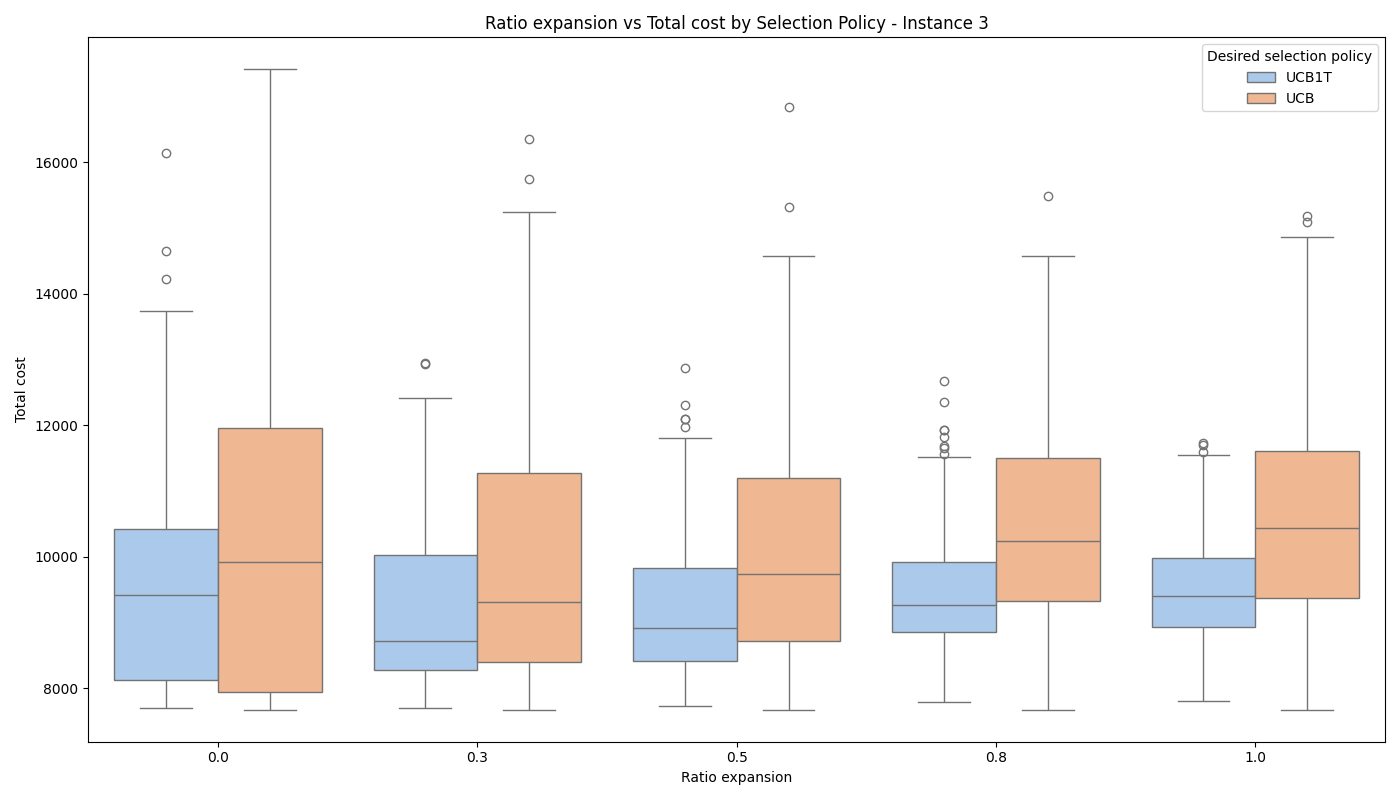
\includegraphics[width=0.42\textwidth]{Figures/3 - ratio_vs_cost.png}
    \caption{Expansion ratio vs Total cost}
    \label{fig:ratio_vs_cost_3}
\end{figure}


\subsubsection*{Analysis of simulations performances}
\begin{figure}[!ht]
    \centering
    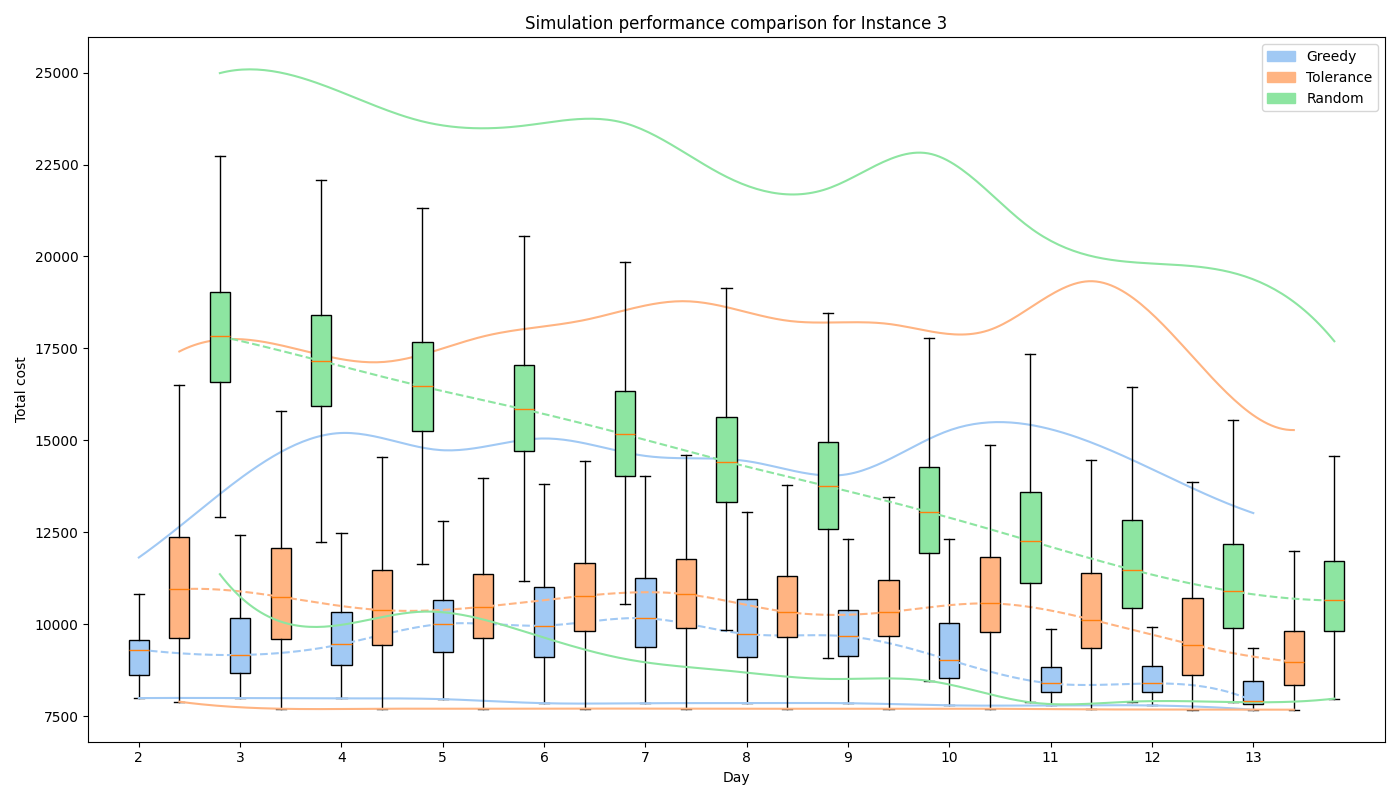
\includegraphics[width=0.42\textwidth]{Figures/3 - Simulation performance.png}
    \caption{Simulation performance - Instance 3}
    \label{fig:sim_perf_3}
\end{figure}
Box plots for the tree simulations policies are represented on Figure \ref{fig:sim_perf_3}. For each day, the distribution of the simulated outcome is plotted regarding the simulation policy. Coloured curves represent the minimum and maximum of these distributions, while dashed lines indicate the medians.

In Figure \ref{fig:sim_perf_3}, the greedy simulation policy is more performant because the distribution of simulations at every day has a lower min, max and median.
The convergence of the Random policy is more pronounced due to the policy's inherent randomness. For instance, with the greedy and tolerance policies, at day two or three, the minimum has already almost been reached. Therefore, a well-calibrated set of parameters for the $\mathcal{MCTS}$ (as defined in Section \ref{sub:notations}) should converge towards the minimum cost found during the simulations. If this is not the case, it indicates that the parameterisation of $\mathcal{MCTS}$ is not optimal. In Figure \ref{fig:sim_perf_4_cp_zero}, the distributions of the simulated outcomes are represented for a  $\mathcal{MCTS}(S_p(C_p=0),E_p(c),R_p,N_c=10)$.


\begin{figure}[!ht]
    \centering
    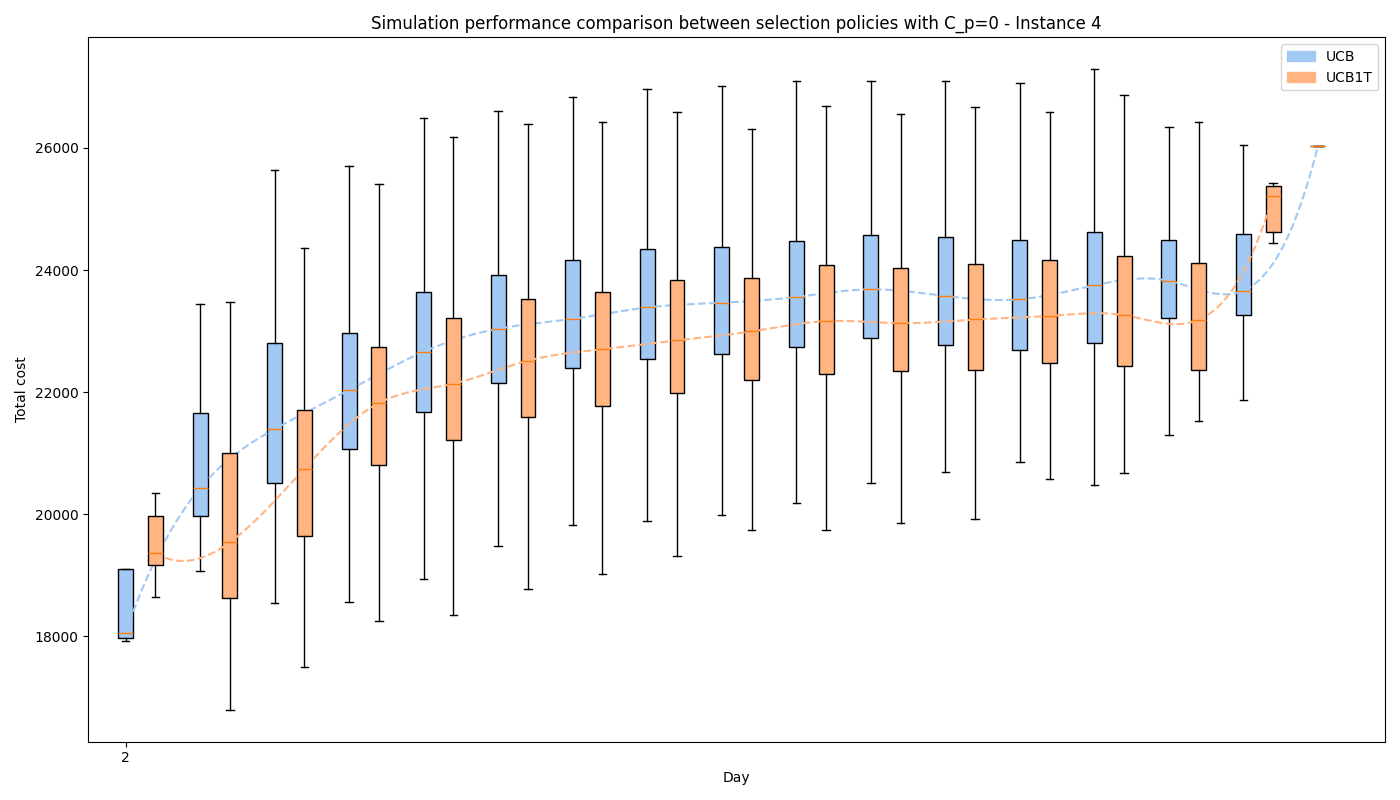
\includegraphics[width=0.42\textwidth]{Figures/4 - Simulation performance - CP=0.png}
    \caption{Simulation performance $C_p=0$ - Instance 4}
    \label{fig:sim_perf_4_cp_zero}
\end{figure}
The parametrisation of this MCTS is not efficient for the considered instance, hence the search process do not converge towards the minimum found cost. These two distributions have a similar behaviour, having $C_p=0$ indicates a similar decision-making process when using the UCB and UCB1T selection policy.
For $I_4$, as mentioned earlier, the difficulty was to run all the simulations of the MCTS with the parameters in the grid search. This is why fewer simulations were carried out for this instance, but we found solutions with a gap of $X\%$ compared to the state-of-the-art solution.

In Figure \ref{fig:sim_perf_vs_c_3}, the median distributions for the different scenarios have been plotted. One can observe that having a value $c$ too close to 1, does not on average converge to this minimum-cost solution. A contrario, lower $c$ values appears to guide the tree search more effectively during the first days of simulations, which is crucial to not overexpand the size of the tree, which can lead to an inefficient and time-consuming MCTS.
\begin{figure}[!ht]
    \centering
    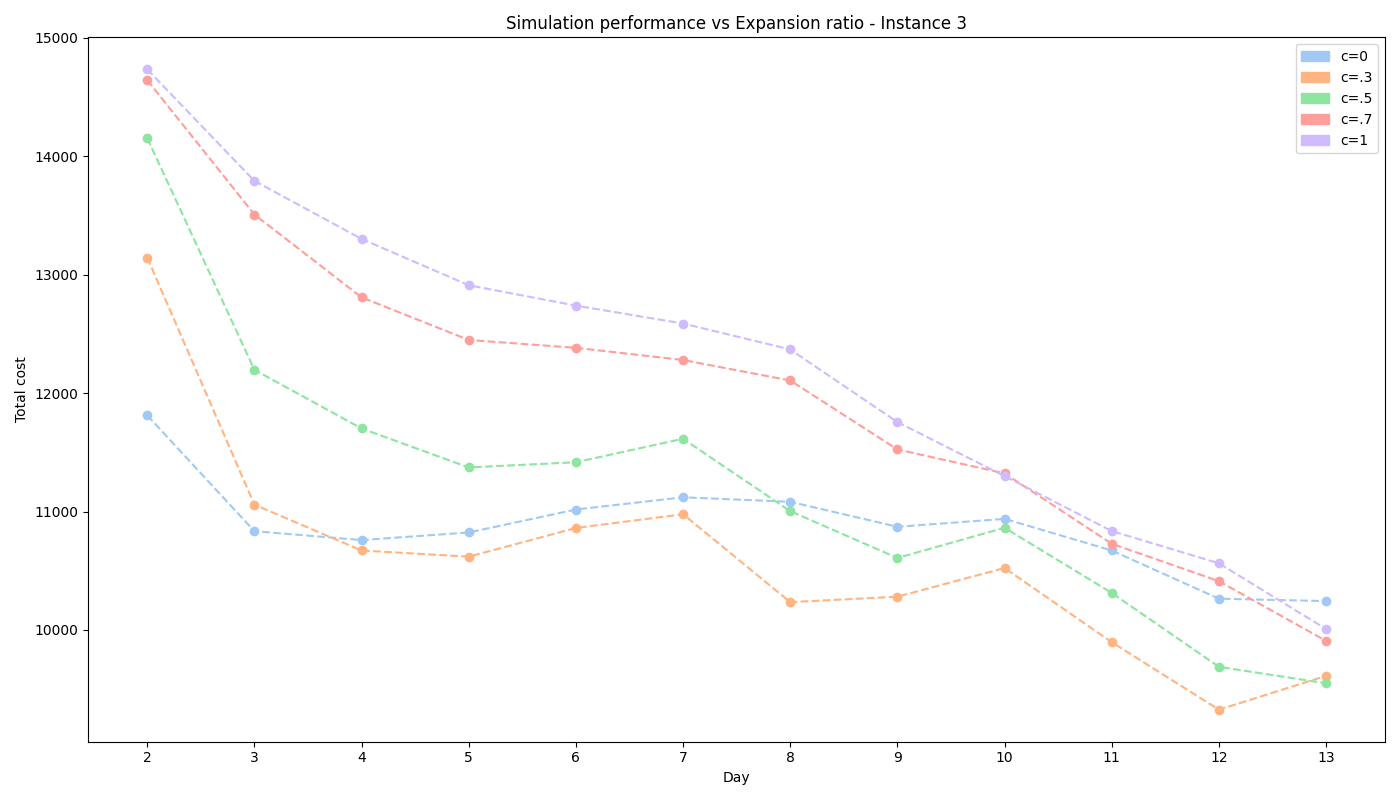
\includegraphics[width=0.42\textwidth]{Figures/3 - Simulation performance vs Expansion ratio.png}
    \caption{Simulation performance vs Expansion Ratio - Instance 3}
    \label{fig:sim_perf_vs_c_3}
\end{figure}

These conclusions can be drawn for small instances, however for $I_4$, we can clearly see in Figure \ref{fig:sim_perf_vs_c_4} that having $c=0$ for a greedy selection policy is inefficient in this tree search because it diverges from the min-simulated cost. The tree search is therefore unable to find a solution after 10 minutes. Based on the median comparison, $c=1$ is a more optimal parameter for guiding the tree search (for $I_3$).
\begin{figure}[!ht]
    \centering
    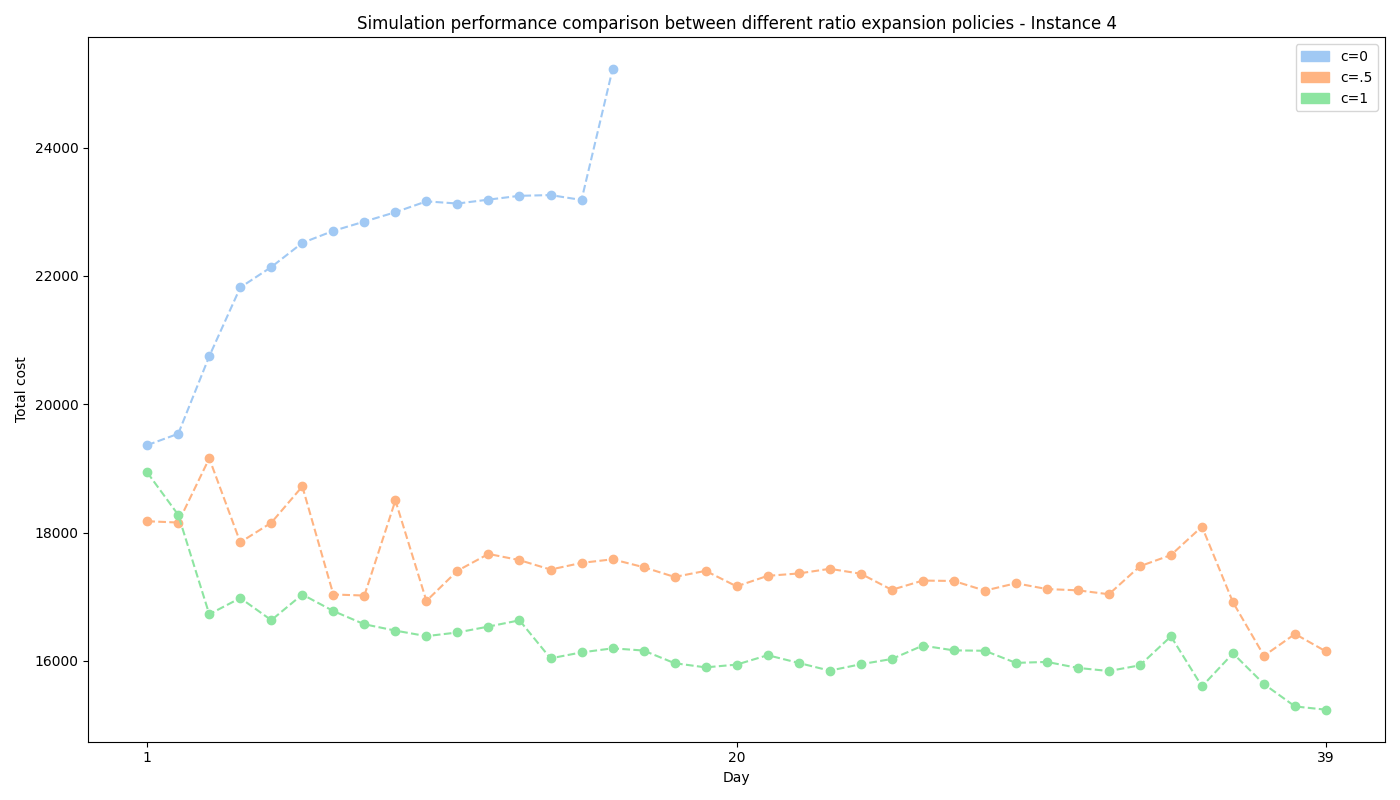
\includegraphics[width=0.42\textwidth]{Figures/4 - Simulation performance vs Expansion ratio.png}
    \caption{Simulation performance vs Expansion Ratio - Instance 4}
    \label{fig:sim_perf_vs_c_4}
\end{figure}


\subsubsection{$I_5$ and $I_6$}

The challenge faced with these two instances is that with the defined grid search, the $\mathcal{MCTS}$ function was not able to conduct the tree search effectively.

While standard stochastic simulation policies can occasionally reach a final state (i.e.\ find a feasible solution), they often fail to guide the search process effectively towards these solutions. Even if the tree expands node's that reached final state, there are few chances to reach a terminal state again, leading to the pruning of the tree.


\subsubsection{$I_7$ and $I_8$}
For $I_7$, we have found solutions close to the best known solution, with a gap of 3.2\%.
The tolerance policy was not in the parameters of the grid search but we run 10 simulations with the parameters defined in Table \ref{table:Simulation table - I7}.

\begin{table}[!ht]
    \centering
    \caption{Simulation table - $I_7$}
    \resizebox{0.45\textwidth}{!}{\begin{tabular}{||>{\centering\arraybackslash}p{1.3cm}
            >{\centering\arraybackslash}p{1.3cm}
            >{\centering\arraybackslash}p{1.3cm}
            >{\centering\arraybackslash}p{1.3cm}
            >{\centering\arraybackslash}p{0.7cm}
            >{\centering\arraybackslash}p{0.8cm}
            >{\centering\arraybackslash}p{1cm}
            >{\centering\arraybackslash}p{1cm}
            >{\centering\arraybackslash}p{1cm}
            >{\centering\arraybackslash}p{1cm}
            ||}
            \toprule
            Selec policy & Exp policy & Simu policy & N° childrens & Ratio & Cp  & Best cost & Mean  & Std  & T(s)  \\
            \midrule
            UCB          & top k      & greedy      & 10           & -     & 1.4 & 31924     & 31924 & 0    & 238.3 \\
            UCB          & ratio k    & greedy      & 10           & .5    & 1.4 & 32331     & 32331 & 0    & 239.7 \\
            UCB          & top k      & tolerance   & 10           & -     & 1.4 & 49712     & 52584 & 1938 & 588.4 \\
            \bottomrule
        \end{tabular}}
    \label{table:Simulation table - I7}
\end{table}

\begin{figure}[!ht]
    \centering
    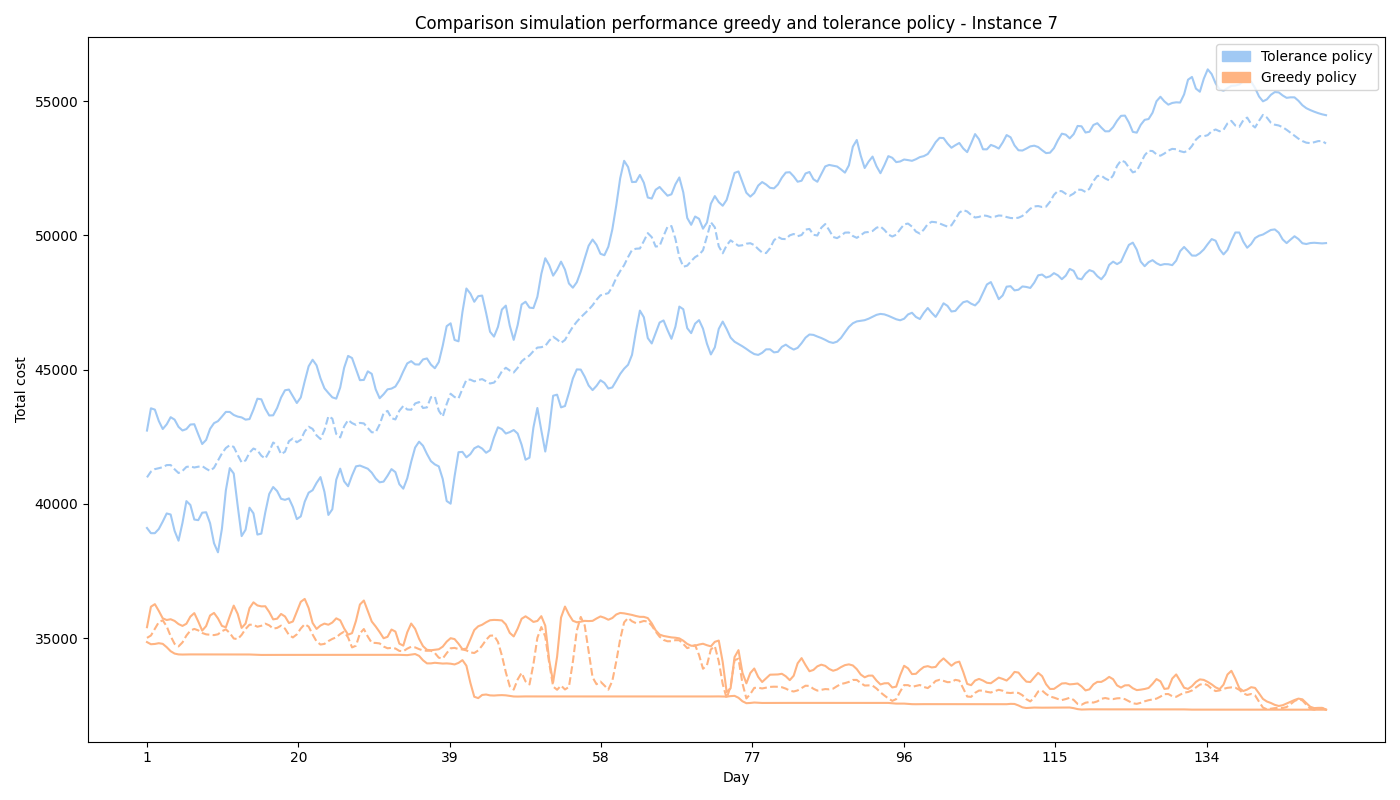
\includegraphics[width=0.42\textwidth]{Figures/7 - comparison sim tolerance vs greedy.png}
    \caption{Simulation performance comparison between Greedy and Tolerance - Instance 7}
    \label{fig:sim_perf_greedy_tolerance_7}
\end{figure}

For this instance, the greedy simulation policy is clearly to be preferred to the tolerance simulation policy. The stochastic policy ends it tree search by selecting nodes that have an overall cost higher than node's found during the simulation process, as shown in Figure \ref{fig:sim_perf_greedy_tolerance_7}. Therefore the parametrisation of $\mathcal{MCTS}$ has to be revised. The ratio\_k and the top\_k policy yields to overall similar performance in term of solution and performance metrics.
Regarding $I_8$, in Table \ref{table:Simulation table - I8}, a new state of the art solution has been found with a with a cost less than 0.52\% compared to the best known solution.
\begin{table}[!ht]
    \centering
    \caption{Simulation table - $I_8$}
    \resizebox{0.45\textwidth}{!}{\begin{tabular}{||>{\centering\arraybackslash}p{1.3cm}
            >{\centering\arraybackslash}p{1.3cm}
            >{\centering\arraybackslash}p{1.3cm}
            >{\centering\arraybackslash}p{1.3cm}
            >{\centering\arraybackslash}p{0.7cm}
            >{\centering\arraybackslash}p{0.8cm}
            >{\centering\arraybackslash}p{1cm}
            >{\centering\arraybackslash}p{1cm}
            >{\centering\arraybackslash}p{1cm}
            >{\centering\arraybackslash}p{1cm}
            ||}
            \toprule
            Selec policy & Exp policy & Simu policy & N° childrens & Ratio & Cp  & Best cost & Mean & Std & T(s)  \\
            \midrule
            UCB          & top k      & greedy      & 10           & -     & 1.4 & 4037      & 4037 & 0   & 718.6 \\
            UCB          & ratio k    & greedy      & 10           & .5    & 1.4 & 4104      & 4104 & 0   & 705.9 \\

            \bottomrule
        \end{tabular}}
    \label{table:Simulation table - I8}
\end{table}




\subsubsection{$I_9$ to $I_{14}$}

Although these instances are outside the scope of this thesis, we have tried to solve them using the same parameters in the grid search as for $I_7$ and $I_8$. The complexity of the instances makes simulations (considering the greedy policy) impossible to reach a final node, as does the problem encountered with $I_5$ and $I_6$.



\subsection{Parallelisation}
As discussed in Section \ref{sub:parralelisation}, parallelisation can be implemented to better estimate one selected node's value.
In our implementation, for $I_4$, we parralelised a $\mathcal{MCTS}(S_p(C_p=0)="UCB",E_p(c=0)="ratio\_k",R_p="random",N_c=10)$ on five cores. The set of parameters has been chosen to represent the behavior of parallelisation in a stochastic environment.  A leaf parralelisation has been implemented, simulating on five cores simultaneously. At every simulation step of the MCTS, the minimum outcome of the five simulations is chosen. 100 simulations of this parralelised MCTS have been runned.

In Figure \ref{fig:sim_perf_parral_4}, the five cores parallelised's distribution better performs than the non-parralelised approach. It confirms that parallelisation guides the MCTS more effectively in the first days of the tree search.

\begin{figure}[!ht]
    \centering
    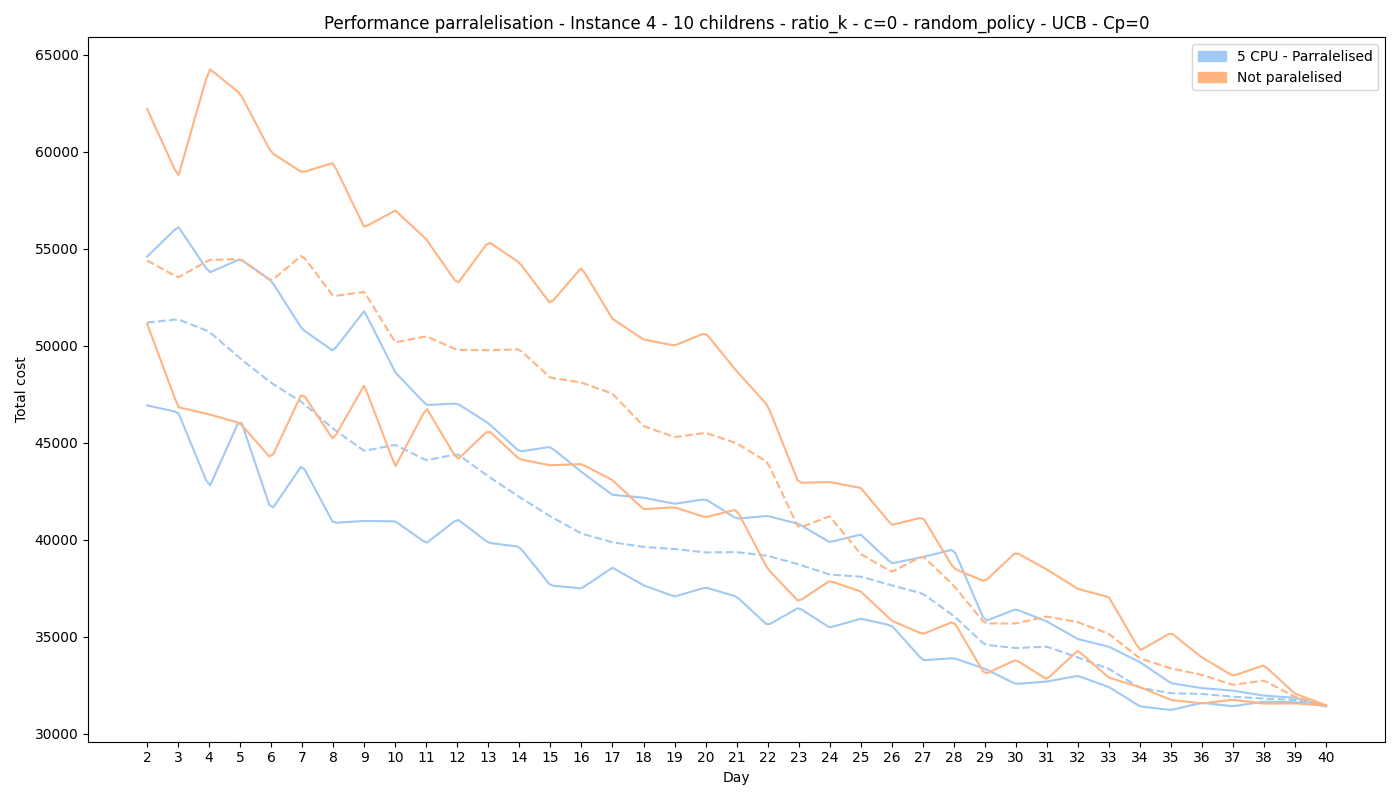
\includegraphics[width=0.42\textwidth]{Figures/4 - Paralelised vs 5 CPU paralelised.png}
    \caption{Comparison of the distributions for the simulated outcomes without parralelisation and with 5 cores - Instance 4}
    \label{fig:sim_perf_parral_4}
\end{figure}

\begin{figure}[!ht]
    \centering
    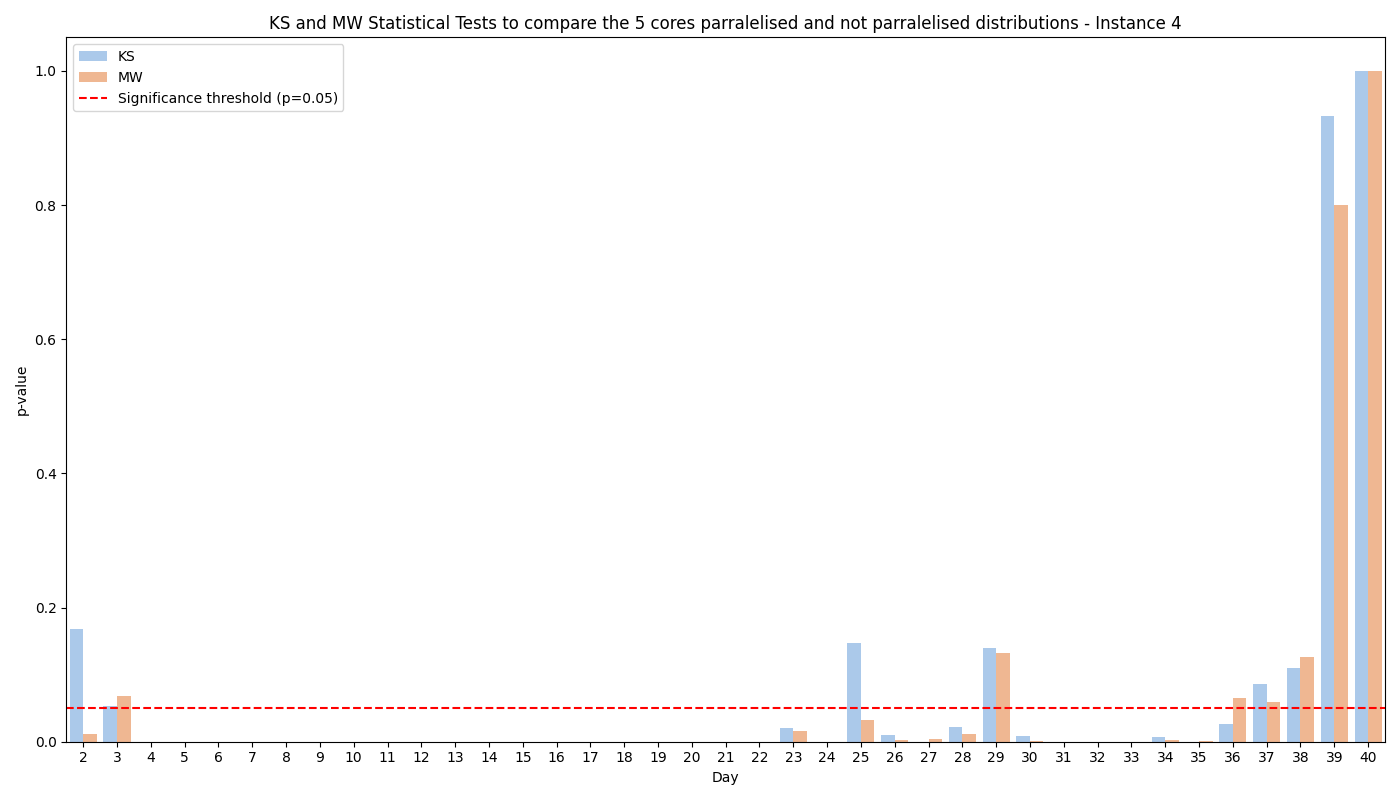
\includegraphics[width=0.42\textwidth]{Figures/Distribution stats tests P vs NP.png}
    \caption{Statistical tests to compare the 5 cores parralelised and not parralelised distribution - Instance 4}
    \label{fig:stats test parralel}
\end{figure}
The Mann-Whitney and the Kolmogorov-Smirnov statistical tests have been implemented. These tests compute p-values that test the null hypothesis that the two groups have the same distribution. Hence, from Figure \ref{fig:stats test parralel} there is enough statistical evidence to say that a five core parallelised MCTS with a stochastic simulation policy better performs with parralelisation at a 5\% level.

A comparison between five-core and ten-core parallelisations of the considered Monte Carlo Tree Search (MCTS) is shown in Figure \ref{fig:parralel (5 vs 10)} and \ref{fig:Stats test 5 VS 10 Parall}. There are no statistical improvments in increasing the number of cores. As discussed in \cite{different_selection_policies}, too many modifications to the MCTS can lead to undesirable behaviour.

\begin{figure}[!ht]
    \centering
    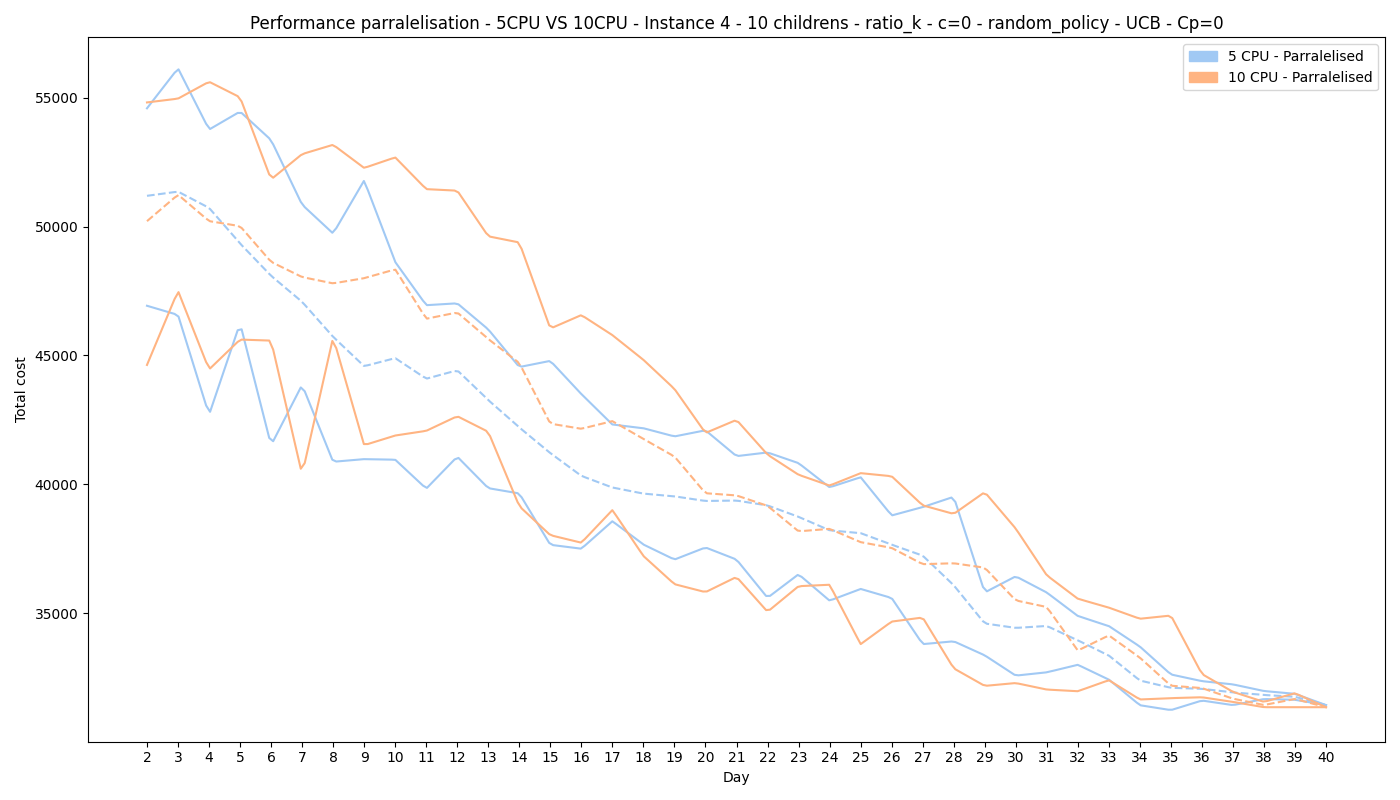
\includegraphics[width=0.42\textwidth]{Figures/4 - 5 CPU Paralelised vs 10 CPU paralelised.png}
    \caption{Comparison of the distributions for the simulated outcomes on 5 vs 10 cores - Instance 4}
    \label{fig:parralel (5 vs 10)}
\end{figure}


\begin{figure}[!ht]
    \centering
    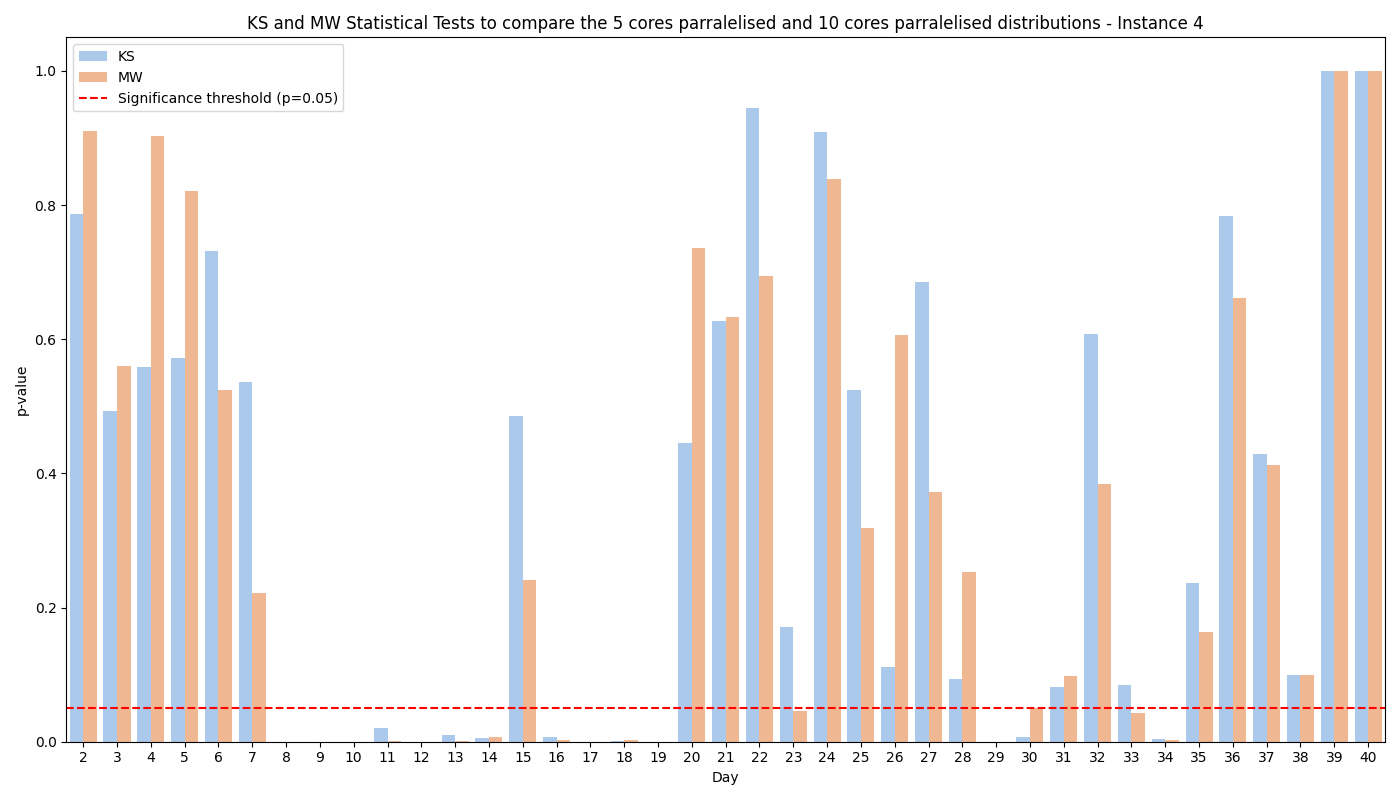
\includegraphics[width=0.42\textwidth]{Figures/4 - Distribution stats tests 5P vs 10P.png}
    \caption{Statistical tests to compare the 5 and 10 cores distribution - Instance 4}
    \label{fig:Stats test 5 VS 10 Parall}
\end{figure}

\onecolumn % Switch to single-column mode

\section{Simulations results}

In these tables, when metrics like the std cannot be computed it is because there are not enough data or because some simulations outputs where NaN. Furthermore, when the expansion policy, Exp policy, is not ratio k, the ratio in the column Ratio is not interpretable because it is not used.

\section*{Instance 1}
\subsection{Solution found}
\begin{center}
  \small
  \begin{longtable}{||>{\centering\arraybackslash}p{1.3cm}
    >{\centering\arraybackslash}p{1.3cm}
    >{\centering\arraybackslash}p{1.3cm}
    >{\centering\arraybackslash}p{1.3cm}
    >{\centering\arraybackslash}p{0.7cm}
    >{\centering\arraybackslash}p{0.8cm}
    >{\centering\arraybackslash}p{1cm}
    >{\centering\arraybackslash}p{1cm}
    >{\centering\arraybackslash}p{1cm}
    >{\centering\arraybackslash}p{1cm}
    ||}
    \toprule
    Selec policy & Exp policy & Simu policy & N° childrens & Ratio & Cp  & Best cost & Mean    & Std     & T(s)   \\
    \midrule
    UCB          & ratio k    & greedy      & 5            & .3    & 2.8 & 1396      & 1396.00 &         & .084   \\
    UCB          & top k      & greedy      & 5            & .5    & 1.4 & 1396      & 1396.00 &         & .085   \\
    UCB          & top k      & greedy      & 5            & .3    & 1.4 & 1396      & 1396.00 &         & .085   \\
    UCB          & top k      & greedy      & 10           & .8    & 1.4 & 1396      & 1396.00 &         & .096   \\
    UCB          & top k      & greedy      & 10           & .3    & 1.4 & 1396      & 1396.00 &         & .097   \\
    UCB          & top k      & greedy      & 5            & .3    & 2.8 & 1396      & 1396.00 &         & .097   \\
    UCB          & top k      & greedy      & 5            & 1     & 1.4 & 1396      & 1396.00 &         & .097   \\
    UCB          & top k      & greedy      & 5            & .8    & 2.8 & 1396      & 1396.00 &         & .098   \\
    UCB          & ratio k    & greedy      & 10           & 1     & 2.8 & 1396      & 1396.00 &         & .098   \\
    UCB          & top k      & greedy      & 5            & 0     & 2.8 & 1396      & 1396.00 &         & .099   \\
    UCB          & ratio k    & greedy      & 5            & 0     & 2.8 & 1396      & 1396.00 &         & .100   \\
    UCB          & ratio k    & greedy      & 5            & 1     & 1.4 & 1396      & 1396.00 &         & .101   \\
    UCB          & top k      & greedy      & 5            & .5    & 2.8 & 1396      & 1396.00 &         & .101   \\
    UCB          & ratio k    & greedy      & 10           & .3    & 2.8 & 1396      & 1396.00 &         & .102   \\
    UCB          & top k      & greedy      & 10           & 0     & 1.4 & 1396      & 1396.00 &         & .103   \\
    UCB          & top k      & greedy      & 15           & .3    & 1.4 & 1396      & 1396.00 &         & .107   \\
    UCB          & top k      & greedy      & 5            & 0     & 1.4 & 1396      & 1396.00 &         & .107   \\
    UCB          & ratio k    & greedy      & 10           & .5    & 2.8 & 1396      & 1396.00 &         & .112   \\
    UCB          & ratio k    & greedy      & 15           & .8    & 1.4 & 1396      & 1396.00 &         & .112   \\
    UCB          & top k      & greedy      & 15           & .8    & 1.4 & 1396      & 1396.00 &         & .115   \\
    UCB          & top k      & greedy      & 15           & 1     & 1.4 & 1396      & 1396.00 &         & .115   \\
    UCB          & ratio k    & greedy      & 10           & 0     & 2.8 & 1396      & 1396.00 &         & .116   \\
    UCB          & top k      & greedy      & 10           & 1     & 1.4 & 1396      & 1396.00 &         & .116   \\
    UCB          & ratio k    & greedy      & 10           & .3    & 1.4 & 1396      & 1396.00 &         & .117   \\
    UCB          & top k      & greedy      & 5            & 1     & 2.8 & 1396      & 1396.00 &         & .117   \\
    UCB          & top k      & greedy      & 15           & .3    & 2.8 & 1396      & 1396.00 &         & .118   \\
    UCB          & top k      & greedy      & 10           & .5    & 1.4 & 1396      & 1396.00 &         & .118   \\
    UCB          & top k      & greedy      & 5            & .8    & 1.4 & 1396      & 1396.00 &         & .118   \\
    UCB          & ratio k    & greedy      & 15           & .3    & 2.8 & 1396      & 1396.00 &         & .119   \\
    UCB          & ratio k    & greedy      & 15           & .8    & 2.8 & 1396      & 1396.00 &         & .119   \\
    UCB          & top k      & greedy      & 15           & .8    & 2.8 & 1396      & 1396.00 &         & .120   \\
    UCB          & ratio k    & greedy      & 10           & .5    & 1.4 & 1396      & 1396.00 &         & .120   \\
    UCB          & ratio k    & tolerance   & 10           & 0     & 2.8 & 1396      & 1396.00 & 0.00    & .120   \\
    UCB          & ratio k    & greedy      & 10           & .8    & 2.8 & 1396      & 1396.00 &         & .122   \\
    UCB          & top k      & greedy      & 15           & 0     & 2.8 & 1396      & 1396.00 &         & .122   \\
    UCB          & top k      & tolerance   & 5            & 0     & 2.8 & 1396      & 1396.00 & 0.00    & .126   \\
    UCB          & top k      & greedy      & 15           & .5    & 1.4 & 1396      & 1396.00 &         & .126   \\
    UCB          & ratio k    & greedy      & 10           & 0     & 1.4 & 1396      & 1396.00 &         & .126   \\
    UCB          & top k      & greedy      & 10           & .8    & 2.8 & 1396      & 1396.00 &         & .127   \\
    UCB          & ratio k    & tolerance   & 15           & 0     & 2.8 & 1396      & 1396.00 & 0.00    & .128   \\
    UCB          & ratio k    & greedy      & 15           & 1     & 2.8 & 1396      & 1396.00 &         & .129   \\
    UCB          & top k      & greedy      & 10           & .3    & 2.8 & 1396      & 1396.00 &         & .131   \\
    UCB          & ratio k    & greedy      & 5            & 1     & 2.8 & 1396      & 1396.00 &         & .131   \\
    UCB          & ratio k    & greedy      & 15           & 0     & 2.8 & 1396      & 1396.00 &         & .132   \\
    UCB          & top k      & greedy      & 10           & 0     & 2.8 & 1396      & 1396.00 &         & .132   \\
    UCB          & ratio k    & greedy      & 15           & .3    & 1.4 & 1396      & 1396.00 &         & .133   \\
    UCB          & ratio k    & greedy      & 15           & .5    & 1.4 & 1396      & 1396.00 &         & .133   \\
    UCB          & top k      & greedy      & 15           & .5    & 2.8 & 1396      & 1396.00 &         & .134   \\
    UCB          & ratio k    & greedy      & 10           & 1     & 1.4 & 1396      & 1396.00 &         & .136   \\
    UCB          & ratio k    & greedy      & 15           & 1     & 1.4 & 1396      & 1396.00 &         & .137   \\
    UCB          & ratio k    & tolerance   & 5            & 0     & 1.4 & 1396      & 1518.60 & 99.08   & .139   \\
    UCB          & top k      & greedy      & 15           & 1     & 2.8 & 1396      & 1396.00 &         & .142   \\
    UCB          & top k      & greedy      & 10           & 1     & 2.8 & 1396      & 1396.00 &         & .143   \\
    UCB          & ratio k    & tolerance   & 15           & 0     & 1.4 & 1396      & 1396.00 & 0.00    & .143   \\
    UCB          & top k      & greedy      & 15           & 0     & 1.4 & 1396      & 1396.00 &         & .143   \\
    UCB          & ratio k    & greedy      & 15           & .5    & 2.8 & 1396      & 1396.00 &         & .147   \\
    UCB          & ratio k    & greedy      & 15           & 0     & 1.4 & 1396      & 1396.00 &         & .148   \\
    UCB          & ratio k    & tolerance   & 10           & 0     & 1.4 & 1396      & 1396.00 & 0.00    & .152   \\
    UCB          & top k      & tolerance   & 15           & 0     & 1.4 & 1396      & 1396.00 & 0.00    & .153   \\
    UCB          & top k      & tolerance   & 10           & 0     & 1.4 & 1396      & 1396.00 & 0.00    & .155   \\
    UCB          & top k      & greedy      & 10           & .5    & 2.8 & 1396      & 1396.00 &         & .157   \\
    UCB          & top k      & tolerance   & 15           & .3    & 2.8 & 1396      & 1524.20 & 72.14   & .157   \\
    UCB          & top k      & tolerance   & 5            & 0     & 1.4 & 1396      & 1396.00 & 0.00    & .158   \\
    UCB          & top k      & tolerance   & 15           & .8    & 1.4 & 1396      & 1654.70 & 185.65  & .161   \\
    UCB          & top k      & tolerance   & 10           & 0     & 2.8 & 1396      & 1396.00 & 0.00    & .174   \\
    UCB          & top k      & tolerance   & 15           & 0     & 2.8 & 1396      & 1396.00 & 0.00    & .177   \\
    UCB          & ratio k    & greedy      & 10           & .8    & 1.4 & 1396      & 1396.00 &         & .178   \\
    UCB          & ratio k    & tolerance   & 15           & .5    & 1.4 & 1396      & 1599.20 & 89.85   & .385   \\
    UCB          & top k      & tolerance   & 5            & .5    & 2.8 & 1396      & 1588.50 & 109.62  & .394   \\
    UCB          & ratio k    & tolerance   & 10           & 1     & 1.4 & 1396      & 1572.20 & 148.00  & .488   \\
    UCB          & top k      & tolerance   & 15           & .8    & 2.8 & 1396      & 1647.80 & 209.03  & .645   \\
    UCB          & ratio k    & tolerance   & 5            & 0     & 2.8 & 1396      & 1509.00 & 81.71   & .659   \\
    UCB          & top k      & tolerance   & 10           & 1     & 1.4 & 1396      & 1617.70 & 183.61  & .794   \\
    UCB          & top k      & tolerance   & 15           & 1     & 2.8 & 1396      & 1589.50 & 130.85  & .809   \\
    UCB          & top k      & tolerance   & 15           & .5    & 2.8 & 1396      & 1528.40 & 109.46  & .837   \\
    UCB          & ratio k    & tolerance   & 15           & 1     & 1.4 & 1396      & 1606.10 & 125.35  & .864   \\
    UCB          & top k      & tolerance   & 5            & .3    & 2.8 & 1396      & 1528.60 & 76.94   & .961   \\
    UCB          & top k      & tolerance   & 10           & .3    & 1.4 & 1396      & 1528.90 & 109.87  & 1.060  \\
    UCB          & ratio k    & tolerance   & 5            & .8    & 1.4 & 1396      & 1574.70 & 123.89  & 1.208  \\
    UCB          & top k      & tolerance   & 15           & 1     & 1.4 & 1396      & 1592.50 & 143.08  & 1.613  \\
    UCB          & ratio k    & random      & 10           & .8    & 0   & 1407      & 3549.90 & 1959.51 & 2.745  \\
    UCB          & top k      & tolerance   & 5            & .3    & 1.4 & 1431      & 1532.50 & 112.31  & .514   \\
    UCB          & top k      & tolerance   & 5            & .8    & 1.4 & 1431      & 1618.70 & 97.18   & .806   \\
    UCB          & ratio k    & tolerance   & 10           & .8    & 1.4 & 1431      & 1583.10 & 123.40  & .830   \\
    UCB          & ratio k    & tolerance   & 10           & .5    & 2.8 & 1431      & 1549.10 & 96.27   & 1.021  \\
    UCB          & ratio k    & tolerance   & 15           & 1     & 2.8 & 1431      & 1615.40 & 179.82  & 1.432  \\
    UCB          & ratio k    & tolerance   & 10           & .3    & 2.8 & 1457      & 1508.70 & 40.06   & .138   \\
    UCB          & top k      & tolerance   & 5            & 1     & 1.4 & 1457      & 1543.60 & 84.48   & 1.857  \\
    UCB          & ratio k    & greedy      & 5            & .5    & 2.8 & 1458      & 1458.00 &         & .113   \\
    UCB          & ratio k    & greedy      & 5            & 0     & 1.4 & 1458      & 1458.00 &         & .115   \\
    UCB          & top k      & tolerance   & 5            & 1     & 2.8 & 1458      & 1563.00 & 88.51   & .126   \\
    UCB          & top k      & tolerance   & 10           & .8    & 2.8 & 1458      & 1640.50 & 101.40  & .348   \\
    UCB          & ratio k    & tolerance   & 15           & .8    & 2.8 & 1458      & 1575.60 & 102.64  & .381   \\
    UCB          & top k      & tolerance   & 10           & .8    & 1.4 & 1458      & 1571.40 & 123.30  & .382   \\
    UCB          & ratio k    & random      & 15           & .8    & 2.8 & 1458      & 4879.30 & 2587.48 & .591   \\
    UCB          & ratio k    & tolerance   & 5            & .8    & 2.8 & 1458      & 1586.00 & 106.15  & .806   \\
    UCB          & top k      & tolerance   & 5            & .5    & 1.4 & 1458      & 1541.30 & 45.20   & .901   \\
    UCB          & ratio k    & tolerance   & 15           & .3    & 2.8 & 1458      & 1502.60 & 63.95   & 1.081  \\
    UCB          & ratio k    & tolerance   & 10           & .5    & 1.4 & 1458      & 1523.70 & 46.63   & 1.161  \\
    UCB          & ratio k    & random      & 10           & 1     & 1.4 & 1458      & 5975.30 & 4237.38 & 1.756  \\
    UCB1T        & ratio k    & greedy      & 10           & .5    & 1.4 & 1472      & 1472.00 &         & .893   \\
    UCB          & top k      & tolerance   & 10           & .8    & 0   & 1472      & 1903.50 & 169.28  & 1.057  \\
    UCB          & ratio k    & tolerance   & 10           & 1     & 2.8 & 1472      & 1661.30 & 160.90  & 1.267  \\
    UCB          & ratio k    & greedy      & 5            & 1     & 0   & 1472      & 1472.00 &         & 1.801  \\
    UCB1T        & ratio k    & tolerance   & 15           & .3    & 1.4 & 1472      & 1818.00 & 150.91  & 5.009  \\
    UCB          & top k      & tolerance   & 15           & .5    & 0   & 1472      & 1808.00 & 146.75  & 5.484  \\
    UCB1T        & top k      & tolerance   & 5            & 0     & 2.8 & 1472      & 1803.50 & 208.94  & 6.320  \\
    UCB          & ratio k    & tolerance   & 5            & 1     & 0   & 1472      & 1799.70 & 161.43  & 6.925  \\
    UCB1T        & ratio k    & tolerance   & 15           & 1     & 0   & 1472      & 1870.00 & 220.25  & 19.040 \\
    UCB1T        & ratio k    & tolerance   & 5            & 1     & 2.8 & 1472      & 1895.10 & 211.12  & 28.132 \\
    UCB          & top k      & tolerance   & 10           & .3    & 2.8 & 1479      & 1520.70 & 70.89   & .160   \\
    UCB          & ratio k    & tolerance   & 5            & .3    & 2.8 & 1479      & 1523.20 & 81.22   & .216   \\
    UCB          & ratio k    & tolerance   & 5            & .3    & 1.4 & 1479      & 1550.20 & 92.04   & .440   \\
    UCB          & top k      & tolerance   & 5            & .8    & 2.8 & 1479      & 1643.70 & 125.43  & .500   \\
    UCB          & ratio k    & tolerance   & 10           & .3    & 1.4 & 1479      & 1560.20 & 65.68   & .870   \\
    UCB          & top k      & tolerance   & 15           & .3    & 1.4 & 1479      & 1561.00 & 73.15   & 1.526  \\
    UCB          & ratio k    & greedy      & 5            & .3    & 1.4 & 1481      & 1481.00 &         & .095   \\
    UCB          & ratio k    & greedy      & 5            & .8    & 2.8 & 1481      & 1481.00 &         & .104   \\
    UCB          & ratio k    & greedy      & 5            & .8    & 1.4 & 1481      & 1481.00 &         & .115   \\
    UCB          & ratio k    & greedy      & 5            & .5    & 1.4 & 1481      & 1481.00 &         & .117   \\
    UCB          & top k      & tolerance   & 15           & .5    & 1.4 & 1481      & 1566.80 & 83.76   & .738   \\
    UCB          & ratio k    & tolerance   & 15           & .3    & 1.4 & 1481      & 1607.00 & 95.21   & 1.236  \\
    UCB1T        & ratio k    & tolerance   & 5            & .8    & 0   & 1481      & 1847.50 & 208.87  & 13.143 \\
    UCB          & ratio k    & tolerance   & 5            & .5    & 2.8 & 1485      & 1559.70 & 90.12   & .644   \\
    UCB          & ratio k    & tolerance   & 5            & 1     & 1.4 & 1489      & 1649.10 & 60.98   & .126   \\
    UCB          & ratio k    & tolerance   & 5            & .5    & 1.4 & 1490      & 1555.70 & 56.12   & .106   \\
    UCB1T        & top k      & tolerance   & 15           & .8    & 0   & 1490      & 1865.60 & 158.48  & 5.096  \\
    UCB1T        & top k      & random      & 5            & .5    & 1.4 & 1493      & 2407.10 & 1045.81 & 3.136  \\
    UCB          & ratio k    & tolerance   & 15           & .5    & 2.8 & 1495      & 1551.60 & 37.38   & .316   \\
    UCB          & top k      & tolerance   & 10           & .5    & 2.8 & 1495      & 1608.60 & 78.12   & 1.129  \\
    UCB          & ratio k    & random      & 5            & 1     & 1.4 & 1506      & 3187.40 & 1785.08 & .179   \\
    UCB          & ratio k    & random      & 5            & 1     & 2.8 & 1506      & 4330.10 & 2775.69 & .492   \\
    UCB          & ratio k    & tolerance   & 15           & .3    & 0   & 1506      & 1745.30 & 193.93  & 1.829  \\
    UCB1T        & top k      & random      & 15           & .3    & 0   & 1506      & 2634.80 & 1495.29 & 2.654  \\
    UCB          & ratio k    & tolerance   & 15           & .8    & 1.4 & 1521      & 1664.60 & 140.50  & .160   \\
    UCB          & top k      & random      & 5            & 0     & 1.4 & 1522      & 3817.40 & 2271.90 & 1.650  \\
    UCB1T        & top k      & tolerance   & 5            & .3    & 1.4 & 1522      & 1803.10 & 135.11  & 44.419 \\
    UCB          & ratio k    & tolerance   & 5            & 1     & 2.8 & 1526      & 1636.10 & 95.27   & .322   \\
    UCB          & ratio k    & tolerance   & 10           & .8    & 2.8 & 1526      & 1658.90 & 95.49   & .654   \\
    UCB1T        & ratio k    & greedy      & 5            & 0     & 1.4 & 1529      & 1529.00 &         & .512   \\
    UCB1T        & ratio k    & random      & 5            & .5    & 1.4 & 1529      & 2613.00 & 1381.25 & .883   \\
    UCB          & top k      & tolerance   & 15           & .3    & 0   & 1529      & 1816.10 & 204.92  & 1.285  \\
    UCB1T        & ratio k    & tolerance   & 5            & 0     & 0   & 1529      & 1889.20 & 191.58  & 2.025  \\
    UCB1T        & ratio k    & random      & 10           & .3    & 1.4 & 1529      & 2922.40 & 1754.56 & 2.695  \\
    UCB1T        & top k      & tolerance   & 15           & 0     & 0   & 1529      & 1884.20 & 166.62  & 2.890  \\
    UCB1T        & ratio k    & tolerance   & 10           & 1     & 0   & 1529      & 1827.00 & 215.19  & 3.312  \\
    UCB1T        & top k      & tolerance   & 15           & .3    & 2.8 & 1529      & 1890.20 & 168.87  & 4.693  \\
    UCB1T        & ratio k    & random      & 15           & .8    & 1.4 & 1529      & 3993.00 & 2298.81 & 5.162  \\
    UCB1T        & top k      & tolerance   & 10           & .5    & 0   & 1529      & 1823.10 & 211.45  & 6.695  \\
    UCB1T        & ratio k    & tolerance   & 10           & .5    & 1.4 & 1529      & 1850.50 & 224.25  & 8.508  \\
    UCB1T        & ratio k    & tolerance   & 10           & .3    & 1.4 & 1529      & 1796.60 & 167.63  & 9.516  \\
    UCB1T        & top k      & tolerance   & 15           & 1     & 0   & 1529      & 1831.70 & 133.56  & 11.001 \\
    UCB1T        & ratio k    & tolerance   & 5            & .8    & 1.4 & 1529      & 1798.40 & 216.53  & 16.114 \\
    UCB          & top k      & tolerance   & 10           & .5    & 1.4 & 1530      & 1609.90 & 76.29   & .924   \\
    UCB1T        & ratio k    & random      & 5            & 0     & 2.8 & 1533      & 3012.00 & 1836.74 & 3.879  \\
    UCB1T        & top k      & tolerance   & 5            & 1     & 0   & 1533      & 1882.40 & 178.26  & 8.601  \\
    UCB1T        & ratio k    & tolerance   & 5            & 1     & 1.4 & 1533      & 1809.70 & 202.15  & 9.562  \\
    UCB1T        & ratio k    & tolerance   & 10           & .8    & 0   & 1533      & 1838.20 & 145.60  & 9.573  \\
    UCB1T        & top k      & tolerance   & 10           & 1     & 0   & 1533      & 1834.90 & 172.42  & 17.707 \\
    UCB1T        & ratio k    & greedy      & 10           & .8    & 0   & 1540      & 1540.00 &         & .666   \\
    UCB1T        & ratio k    & greedy      & 10           & 1     & 0   & 1540      & 1540.00 &         & .879   \\
    UCB1T        & top k      & random      & 15           & .5    & 2.8 & 1540      & 3122.70 & 1753.55 & 1.088  \\
    UCB1T        & top k      & greedy      & 15           & .5    & 2.8 & 1540      & 1540.00 &         & 1.181  \\
    UCB1T        & ratio k    & tolerance   & 5            & .3    & 0   & 1540      & 1864.60 & 175.12  & 1.319  \\
    UCB1T        & top k      & greedy      & 15           & .8    & 2.8 & 1540      & 1540.00 &         & 1.664  \\
    UCB          & top k      & greedy      & 5            & .5    & 0   & 1540      & 1540.00 &         & 1.694  \\
    UCB          & top k      & greedy      & 5            & 0     & 0   & 1540      & 1540.00 &         & 1.702  \\
    UCB1T        & ratio k    & tolerance   & 10           & .8    & 1.4 & 1540      & 1845.80 & 162.15  & 2.461  \\
    UCB1T        & top k      & greedy      & 5            & .3    & 1.4 & 1540      & 1540.00 &         & 2.500  \\
    UCB          & top k      & tolerance   & 5            & .5    & 0   & 1540      & 1800.30 & 156.39  & 2.706  \\
    UCB1T        & ratio k    & tolerance   & 10           & .3    & 0   & 1540      & 1831.40 & 174.19  & 2.958  \\
    UCB1T        & top k      & tolerance   & 15           & .3    & 0   & 1540      & 1896.80 & 214.92  & 3.424  \\
    UCB          & ratio k    & tolerance   & 10           & 0     & 0   & 1540      & 1850.20 & 183.61  & 4.229  \\
    UCB1T        & ratio k    & tolerance   & 5            & .3    & 2.8 & 1540      & 1919.00 & 194.58  & 5.013  \\
    UCB1T        & top k      & tolerance   & 15           & 0     & 2.8 & 1540      & 1865.30 & 202.86  & 5.138  \\
    UCB1T        & top k      & tolerance   & 10           & .5    & 2.8 & 1540      & 1776.30 & 180.87  & 6.638  \\
    UCB          & ratio k    & tolerance   & 15           & 0     & 0   & 1540      & 1913.30 & 207.39  & 7.511  \\
    UCB1T        & top k      & tolerance   & 10           & .5    & 1.4 & 1540      & 1885.00 & 235.90  & 7.624  \\
    UCB          & top k      & tolerance   & 15           & .8    & 0   & 1540      & 1810.70 & 162.48  & 7.951  \\
    UCB          & top k      & tolerance   & 10           & 0     & 0   & 1540      & 1882.00 & 169.58  & 8.397  \\
    UCB1T        & ratio k    & tolerance   & 10           & .3    & 2.8 & 1540      & 1786.20 & 149.51  & 9.080  \\
    UCB1T        & ratio k    & tolerance   & 15           & .8    & 2.8 & 1540      & 1758.30 & 183.71  & 9.664  \\
    UCB1T        & top k      & tolerance   & 15           & 1     & 2.8 & 1540      & 1814.90 & 116.59  & 9.710  \\
    UCB1T        & ratio k    & tolerance   & 15           & 1     & 2.8 & 1540      & 1862.50 & 184.05  & 9.835  \\
    UCB1T        & ratio k    & tolerance   & 15           & .3    & 0   & 1540      & 1809.80 & 164.19  & 10.175 \\
    UCB1T        & ratio k    & tolerance   & 10           & 1     & 2.8 & 1540      & 1897.00 & 281.85  & 10.565 \\
    UCB1T        & ratio k    & tolerance   & 15           & .8    & 1.4 & 1540      & 1908.50 & 196.92  & 13.413 \\
    UCB1T        & ratio k    & tolerance   & 15           & .5    & 1.4 & 1540      & 1868.40 & 160.08  & 15.130 \\
    UCB1T        & top k      & tolerance   & 5            & .8    & 0   & 1540      & 1824.20 & 165.59  & 16.175 \\
    UCB1T        & top k      & tolerance   & 5            & 0     & 1.4 & 1540      & 1806.50 & 198.51  & 17.011 \\
    UCB1T        & top k      & tolerance   & 5            & .3    & 0   & 1540      & 1870.70 & 196.15  & 22.181 \\
    UCB1T        & top k      & tolerance   & 5            & 0     & 0   & 1540      & 1732.90 & 156.80  & 35.029 \\
    UCB1T        & top k      & tolerance   & 5            & .5    & 2.8 & 1540      & 1828.10 & 128.77  & 53.816 \\
    UCB          & ratio k    & random      & 15           & .8    & 0   & 1544      & 3538.60 & 1864.08 & 1.304  \\
    UCB1T        & top k      & random      & 5            & 0     & 2.8 & 1544      & 2510.60 & 969.95  & 1.983  \\
    UCB1T        & top k      & tolerance   & 15           & .3    & 1.4 & 1546      & 1832.00 & 184.84  & 3.920  \\
    UCB          & top k      & tolerance   & 10           & 1     & 2.8 & 1547      & 1639.00 & 101.50  & .350   \\
    UCB          & top k      & random      & 15           & .3    & 2.8 & 1548      & 7304.10 & 5361.45 & 1.066  \\
    UCB1T        & top k      & tolerance   & 15           & .5    & 0   & 1548      & 1838.50 & 129.02  & 5.476  \\
    UCB1T        & top k      & tolerance   & 10           & .3    & 0   & 1548      & 1959.70 & 210.51  & 20.794 \\
    UCB1T        & ratio k    & random      & 15           & 0     & 0   & 1551      & 2592.00 & 1259.81 & 2.241  \\
    UCB1T        & top k      & tolerance   & 15           & .8    & 2.8 & 1551      & 1862.00 & 139.22  & 12.043 \\
    UCB1T        & ratio k    & tolerance   & 5            & 1     & 0   & 1551      & 1884.40 & 202.74  & 22.815 \\
    UCB          & ratio k    & tolerance   & 5            & .5    & 0   & 1552      & 1861.00 & 177.52  & 1.938  \\
    UCB          & ratio k    & tolerance   & 5            & .8    & 0   & 1552      & 1818.80 & 158.49  & 2.109  \\
    UCB1T        & top k      & tolerance   & 10           & 1     & 2.8 & 1552      & 1826.90 & 170.80  & 7.951  \\
    UCB1T        & ratio k    & tolerance   & 5            & .5    & 0   & 1553      & 1842.90 & 145.37  & 1.425  \\
    UCB1T        & ratio k    & tolerance   & 5            & .5    & 2.8 & 1553      & 1820.10 & 155.51  & 3.897  \\
    UCB1T        & top k      & random      & 10           & 0     & 2.8 & 1553      & 3300.10 & 1765.23 & 3.970  \\
    UCB          & ratio k    & tolerance   & 10           & .8    & 0   & 1553      & 1865.80 & 179.46  & 5.543  \\
    UCB1T        & ratio k    & tolerance   & 15           & 0     & 2.8 & 1553      & 1842.80 & 230.98  & 5.783  \\
    UCB1T        & ratio k    & tolerance   & 10           & .5    & 0   & 1553      & 1832.90 & 113.14  & 9.797  \\
    UCB1T        & ratio k    & tolerance   & 15           & .5    & 0   & 1553      & 1853.50 & 165.94  & 12.827 \\
    UCB1T        & top k      & random      & 5            & .5    & 0   & 1555      & 2709.90 & 1386.28 & .908   \\
    UCB1T        & top k      & random      & 15           & .3    & 1.4 & 1555      & 2758.60 & 1549.45 & 5.773  \\
    UCB1T        & top k      & tolerance   & 10           & .8    & 0   & 1561      & 1842.40 & 185.52  & 4.651  \\
    UCB1T        & ratio k    & tolerance   & 15           & .5    & 2.8 & 1561      & 1886.10 & 209.51  & 8.565  \\
    UCB          & ratio k    & tolerance   & 10           & 1     & 0   & 1564      & 1792.40 & 163.67  & .729   \\
    UCB          & top k      & greedy      & 10           & .5    & 0   & 1564      & 1564.00 &         & .746   \\
    UCB1T        & ratio k    & greedy      & 10           & 1     & 1.4 & 1564      & 1564.00 &         & .967   \\
    UCB1T        & ratio k    & greedy      & 15           & .3    & 1.4 & 1564      & 1564.00 &         & 1.123  \\
    UCB1T        & top k      & tolerance   & 10           & .3    & 2.8 & 1564      & 1848.00 & 154.42  & 1.583  \\
    UCB1T        & top k      & tolerance   & 10           & 0     & 2.8 & 1564      & 1876.20 & 146.84  & 2.413  \\
    UCB          & ratio k    & tolerance   & 10           & .3    & 0   & 1564      & 1894.60 & 168.37  & 3.180  \\
    UCB1T        & ratio k    & tolerance   & 15           & 0     & 1.4 & 1564      & 1926.10 & 169.41  & 3.914  \\
    UCB1T        & ratio k    & tolerance   & 10           & 0     & 0   & 1564      & 1894.10 & 209.84  & 5.046  \\
    UCB          & top k      & tolerance   & 5            & .3    & 0   & 1564      & 1802.20 & 110.06  & 5.248  \\
    UCB1T        & ratio k    & tolerance   & 10           & .5    & 2.8 & 1564      & 1903.40 & 202.94  & 5.620  \\
    UCB          & top k      & tolerance   & 15           & 0     & 0   & 1564      & 1996.80 & 188.44  & 7.431  \\
    UCB1T        & top k      & tolerance   & 15           & .5    & 1.4 & 1564      & 1801.10 & 181.31  & 8.398  \\
    UCB          & top k      & tolerance   & 5            & .8    & 0   & 1564      & 1821.10 & 171.24  & 8.987  \\
    UCB1T        & top k      & tolerance   & 15           & 1     & 1.4 & 1564      & 1857.30 & 200.71  & 10.041 \\
    UCB1T        & ratio k    & tolerance   & 15           & 1     & 1.4 & 1564      & 1931.50 & 183.48  & 12.772 \\
    UCB1T        & top k      & tolerance   & 5            & .5    & 1.4 & 1564      & 1891.70 & 149.04  & 31.446 \\
    UCB          & ratio k    & random      & 10           & .3    & 2.8 & 1565      & 5063.80 & 4094.92 & .375   \\
    UCB1T        & top k      & random      & 10           & .3    & 0   & 1565      & 3329.80 & 2124.79 & 2.699  \\
    UCB1T        & top k      & random      & 15           & 1     & 0   & 1565      & 3236.20 & 2047.21 & 5.953  \\
    UCB1T        & top k      & random      & 10           & 1     & 2.8 & 1569      & 2779.10 & 1889.48 & 1.492  \\
    UCB          & ratio k    & random      & 15           & .3    & 2.8 & 1577      & 6779.70 & 3457.07 & 1.545  \\
    UCB1T        & top k      & tolerance   & 10           & 0     & 0   & 1577      & 1873.80 & 178.43  & 2.373  \\
    UCB1T        & ratio k    & random      & 15           & 1     & 0   & 1577      & 3337.20 & 1588.71 & 5.721  \\
    UCB1T        & ratio k    & random      & 10           & 1     & 0   & 1577      & 2901.20 & 1262.22 & 5.992  \\
    UCB1T        & top k      & tolerance   & 5            & .3    & 2.8 & 1578      & 1838.70 & 131.18  & 30.039 \\
    UCB1T        & top k      & tolerance   & 10           & .8    & 2.8 & 1580      & 1939.40 & 235.60  & 4.992  \\
    UCB          & top k      & random      & 15           & .8    & 2.8 & 1583      & 3255.00 & 1757.31 & .794   \\
    UCB          & top k      & random      & 5            & .3    & 0   & 1583      & 3648.60 & 2136.03 & 1.634  \\
    UCB          & top k      & random      & 10           & 1     & 0   & 1583      & 3451.60 & 2094.03 & 3.372  \\
    UCB          & ratio k    & random      & 5            & .5    & 2.8 & 1588      & 5819.70 & 3215.99 & .441   \\
    UCB1T        & ratio k    & random      & 10           & .8    & 1.4 & 1591      & 3953.30 & 2378.61 & 2.344  \\
    UCB          & ratio k    & random      & 5            & .8    & 1.4 & 1602      & 3413.60 & 1617.10 & .687   \\
    UCB1T        & top k      & random      & 15           & .8    & 0   & 1606      & 3215.40 & 1457.51 & 2.597  \\
    UCB1T        & ratio k    & random      & 10           & .5    & 0   & 1615      & 2917.70 & 1738.06 & 1.223  \\
    UCB1T        & top k      & random      & 5            & 0     & 1.4 & 1615      & 2243.60 & 798.90  & 2.994  \\
    UCB1T        & top k      & random      & 15           & .8    & 1.4 & 1615      & 3428.80 & 2035.35 & 3.857  \\
    UCB1T        & top k      & random      & 10           & 0     & 0   & 1623      & 4175.70 & 2223.66 & 3.049  \\
    UCB1T        & ratio k    & greedy      & 5            & .3    & 0   & 1624      & 1624.00 &         & .749   \\
    UCB          & top k      & random      & 5            & 1     & 1.4 & 1627      & 3999.30 & 2670.48 & .513   \\
    UCB          & top k      & random      & 5            & 0     & 0   & 1629      & 2414.10 & 1280.07 & .261   \\
    UCB1T        & top k      & random      & 5            & 1     & 2.8 & 1633      & 2838.30 & 1236.17 & 3.507  \\
    UCB1T        & ratio k    & random      & 5            & 1     & 2.8 & 1644      & 3006.80 & 1803.40 & .479   \\
    UCB          & top k      & random      & 15           & 1     & 0   & 1647      & 2351.30 & 1096.41 & 1.609  \\
    UCB          & top k      & random      & 15           & .3    & 1.4 & 1651      & 3986.00 & 2543.37 & 1.927  \\
    UCB1T        & ratio k    & random      & 5            & .8    & 1.4 & 1651      & 2863.80 & 1129.95 & 3.658  \\
    UCB          & top k      & random      & 10           & 0     & 0   & 1658      & 2117.20 & 621.46  & 3.543  \\
    UCB1T        & ratio k    & random      & 5            & .5    & 0   & 1659      & 4723.70 & 1707.27 & 3.918  \\
    UCB          & top k      & random      & 10           & 1     & 2.8 & 1660      & 4102.50 & 2659.39 & .610   \\
    UCB1T        & top k      & tolerance   & 5            & .8    & 1.4 & 1660      & 1874.60 & 188.31  & 47.533 \\
    UCB1T        & ratio k    & random      & 10           & .8    & 0   & 1661      & 3054.30 & 1542.70 & 1.292  \\
    UCB          & top k      & random      & 10           & .8    & 2.8 & 1661      & 4508.90 & 3139.63 & 1.591  \\
    UCB1T        & ratio k    & random      & 5            & .8    & 0   & 1662      & 1940.40 & 231.25  & 4.169  \\
    UCB1T        & ratio k    & tolerance   & 5            & .8    & 2.8 & 1662      & 1837.90 & 117.26  & 6.998  \\
    UCB1T        & ratio k    & greedy      & 5            & .3    & 1.4 & 1663      & 1663.00 &         & .480   \\
    UCB          & ratio k    & tolerance   & 5            & .3    & 0   & 1663      & 1865.90 & 178.68  & 1.407  \\
    UCB          & ratio k    & random      & 10           & 1     & 2.8 & 1663      & 4552.30 & 3487.52 & 1.795  \\
    UCB1T        & ratio k    & tolerance   & 5            & 0     & 2.8 & 1663      & 1927.80 & 140.83  & 3.367  \\
    UCB1T        & top k      & tolerance   & 15           & .5    & 2.8 & 1663      & 1829.20 & 105.51  & 4.329  \\
    UCB1T        & ratio k    & random      & 10           & .3    & 2.8 & 1663      & 3892.50 & 2094.32 & 4.499  \\
    UCB          & top k      & tolerance   & 5            & 0     & 0   & 1663      & 1838.30 & 154.11  & 9.751  \\
    UCB1T        & ratio k    & random      & 10           & 0     & 0   & 1666      & 2367.30 & 814.70  & 1.318  \\
    UCB          & ratio k    & random      & 5            & .3    & 2.8 & 1666      & 5948.00 & 4768.95 & 1.669  \\
    UCB1T        & ratio k    & tolerance   & 5            & .3    & 1.4 & 1666      & 1941.90 & 195.48  & 7.231  \\
    UCB1T        & top k      & tolerance   & 15           & 0     & 1.4 & 1666      & 1904.90 & 142.41  & 9.858  \\
    UCB1T        & top k      & random      & 15           & .8    & 2.8 & 1668      & 2303.00 & 1087.21 & 4.729  \\
    UCB1T        & ratio k    & random      & 10           & .3    & 0   & 1673      & 3451.40 & 2083.35 & 4.420  \\
    UCB          & top k      & tolerance   & 10           & 1     & 0   & 1674      & 1853.70 & 131.34  & 2.065  \\
    UCB1T        & top k      & tolerance   & 10           & 1     & 1.4 & 1674      & 1878.20 & 129.77  & 5.518  \\
    UCB          & top k      & random      & 5            & 1     & 0   & 1678      & 2416.90 & 959.20  & 1.502  \\
    UCB1T        & ratio k    & tolerance   & 10           & 0     & 1.4 & 1678      & 1914.00 & 147.42  & 3.342  \\
    UCB          & top k      & tolerance   & 5            & 1     & 0   & 1678      & 1867.30 & 151.01  & 3.844  \\
    UCB          & ratio k    & random      & 5            & .5    & 1.4 & 1681      & 5446.30 & 3691.78 & .327   \\
    UCB          & ratio k    & tolerance   & 10           & .5    & 0   & 1689      & 1904.90 & 154.68  & 2.938  \\
    UCB1T        & top k      & random      & 10           & .5    & 1.4 & 1689      & 2506.30 & 1778.12 & 4.497  \\
    UCB1T        & ratio k    & greedy      & 15           & .3    & 0   & 1690      & 1690.00 &         & 1.255  \\
    UCB          & top k      & random      & 15           & .5    & 2.8 & 1691      & 7503.60 & 5126.19 & 1.821  \\
    UCB          & top k      & random      & 5            & .3    & 1.4 & 1695      & 4332.60 & 2620.35 & .510   \\
    UCB          & ratio k    & tolerance   & 5            & 0     & 0   & 1695      & 1905.40 & 153.02  & 3.821  \\
    UCB          & ratio k    & tolerance   & 15           & 1     & 0   & 1695      & 1890.90 & 135.28  & 6.258  \\
    UCB1T        & ratio k    & tolerance   & 10           & 1     & 1.4 & 1695      & 1859.40 & 127.66  & 6.288  \\
    UCB1T        & ratio k    & random      & 5            & .5    & 2.8 & 1696      & 2727.90 & 1650.15 & 2.736  \\
    UCB1T        & ratio k    & random      & 15           & 0     & 2.8 & 1698      & 3103.20 & 2377.88 & 1.629  \\
    UCB1T        & top k      & greedy      & 5            & .8    & 2.8 & 1698      & 1698.00 &         & 3.695  \\
    UCB1T        & top k      & random      & 10           & .8    & 0   & 1698      & 2707.90 & 1578.17 & 4.028  \\
    UCB1T        & top k      & tolerance   & 5            & 1     & 2.8 & 1698      & 1864.90 & 122.14  & 35.399 \\
    UCB          & ratio k    & random      & 10           & .5    & 1.4 & 1703      & 3470.90 & 2151.66 & .579   \\
    UCB          & ratio k    & random      & 10           & .3    & 1.4 & 1704      & 4665.60 & 2019.66 & .354   \\
    UCB          & top k      & random      & 10           & .5    & 1.4 & 1704      & 5167.30 & 2683.04 & .807   \\
    UCB          & top k      & random      & 5            & .8    & 1.4 & 1706      & 3614.60 & 1951.29 & .381   \\
    UCB          & top k      & random      & 5            & .5    & 1.4 & 1706      & 4569.00 & 2297.57 & 1.213  \\
    UCB1T        & top k      & tolerance   & 10           & .8    & 1.4 & 1708      & 1906.30 & 132.86  & 2.060  \\
    UCB          & top k      & random      & 5            & .5    & 0   & 1709      & 2336.70 & 1046.92 & 1.765  \\
    UCB1T        & top k      & random      & 5            & .3    & 0   & 1709      & 3106.80 & 1567.96 & 2.854  \\
    UCB1T        & ratio k    & tolerance   & 15           & .8    & 0   & 1710      & 1881.00 & 143.86  & 15.660 \\
    UCB          & top k      & greedy      & 10           & .3    & 0   & 1711      & 1711.00 &         & .738   \\
    UCB          & ratio k    & random      & 5            & .5    & 0   & 1715      & 3376.90 & 2127.71 & 1.448  \\
    UCB1T        & ratio k    & random      & 15           & .5    & 1.4 & 1717      & 3660.50 & 2148.20 & 4.281  \\
    UCB1T        & top k      & random      & 5            & 1     & 0   & 1718      & 3008.10 & 1546.53 & 1.967  \\
    UCB1T        & top k      & greedy      & 5            & .5    & 2.8 & 1720      & 1720.00 &         & 3.694  \\
    UCB1T        & top k      & tolerance   & 5            & .5    & 0   & 1720      & 1858.30 & 108.43  & 5.149  \\
    UCB1T        & ratio k    & random      & 15           & .8    & 0   & 1720      & 3732.40 & 1699.79 & 6.089  \\
    UCB1T        & top k      & random      & 10           & .3    & 2.8 & 1724      & 2674.40 & 1285.84 & 3.201  \\
    UCB1T        & top k      & random      & 5            & .8    & 2.8 & 1726      & 2636.60 & 1126.54 & 1.093  \\
    UCB          & ratio k    & random      & 5            & 0     & 1.4 & 1728      & 4667.50 & 2998.11 & .755   \\
    UCB          & ratio k    & random      & 10           & 0     & 2.8 & 1729      & 5947.60 & 3119.40 & 1.541  \\
    UCB1T        & top k      & tolerance   & 5            & 1     & 1.4 & 1729      & 1885.90 & 169.41  & 34.003 \\
    UCB1T        & top k      & random      & 10           & 1     & 0   & 1730      & 3578.90 & 2090.43 & .633   \\
    UCB          & ratio k    & random      & 15           & 1     & 0   & 1730      & 2956.50 & 1754.33 & 2.322  \\
    UCB1T        & ratio k    & greedy      & 15           & 1     & 0   & 1734      & 1734.00 &         & 1.119  \\
    UCB          & top k      & random      & 10           & .3    & 1.4 & 1734      & 6041.60 & 3811.51 & 1.387  \\
    UCB          & ratio k    & tolerance   & 15           & .8    & 0   & 1734      & 1937.30 & 160.39  & 2.265  \\
    UCB1T        & top k      & tolerance   & 10           & .3    & 1.4 & 1740      & 1937.60 & 141.06  & 5.471  \\
    UCB1T        & top k      & greedy      & 10           & .8    & 0   & 1741      & 1741.00 &         & .881   \\
    UCB1T        & ratio k    & random      & 10           & .5    & 2.8 & 1741      & 3925.10 & 2795.34 & 5.267  \\
    UCB          & top k      & tolerance   & 10           & .5    & 0   & 1741      & 1849.90 & 89.06   & 6.946  \\
    UCB1T        & ratio k    & tolerance   & 15           & .3    & 2.8 & 1741      & 1966.30 & 171.06  & 15.788 \\
    UCB          & top k      & random      & 5            & .3    & 2.8 & 1742      & 5442.90 & 2963.68 & .342   \\
    UCB          & top k      & greedy      & 5            & .3    & 0   & 1742      & 1742.00 &         & 1.340  \\
    UCB1T        & ratio k    & random      & 15           & 0     & 1.4 & 1743      & 3496.30 & 1585.15 & 2.786  \\
    UCB1T        & top k      & random      & 10           & .3    & 1.4 & 1744      & 2799.80 & 1512.75 & 3.386  \\
    UCB1T        & ratio k    & tolerance   & 10           & .8    & 2.8 & 1744      & 1942.20 & 114.58  & 7.479  \\
    UCB          & top k      & tolerance   & 15           & 1     & 0   & 1745      & 1888.90 & 110.64  & 2.671  \\
    UCB1T        & top k      & random      & 15           & .3    & 2.8 & 1746      & 3621.40 & 1663.32 & .667   \\
    UCB1T        & top k      & random      & 15           & .5    & 0   & 1746      & 3835.00 & 1661.25 & 5.242  \\
    UCB1T        & top k      & random      & 5            & .3    & 1.4 & 1748      & 2388.70 & 1026.37 & .811   \\
    UCB          & ratio k    & random      & 5            & .8    & 0   & 1752      & 3143.70 & 1727.99 & .330   \\
    UCB          & top k      & random      & 10           & 0     & 1.4 & 1752      & 6513.10 & 2763.61 & .388   \\
    UCB1T        & ratio k    & greedy      & 15           & .3    & 2.8 & 1752      & 1752.00 &         & .822   \\
    UCB          & top k      & random      & 15           & .3    & 0   & 1752      & 2640.80 & 1776.83 & .905   \\
    UCB1T        & ratio k    & random      & 5            & .8    & 2.8 & 1752      & 2631.00 & 1651.86 & 1.930  \\
    UCB1T        & top k      & random      & 15           & 0     & 0   & 1754      & 3047.90 & 1422.93 & 4.130  \\
    UCB1T        & top k      & random      & 15           & 0     & 1.4 & 1755      & 3598.20 & 1915.88 & .549   \\
    UCB1T        & ratio k    & random      & 10           & .8    & 2.8 & 1755      & 3665.50 & 1700.67 & 4.641  \\
    UCB          & ratio k    & greedy      & 5            & .3    & 0   & 1757      & 1757.00 &         & .308   \\
    UCB1T        & ratio k    & random      & 15           & .3    & 0   & 1758      & 3812.60 & 1938.27 & 1.372  \\
    UCB1T        & top k      & greedy      & 15           & 1     & 1.4 & 1759      & 1759.00 &         & 1.236  \\
    UCB1T        & top k      & random      & 10           & .5    & 0   & 1767      & 3736.40 & 2107.52 & 3.212  \\
    UCB          & ratio k    & random      & 15           & .5    & 0   & 1771      & 2491.90 & 1254.11 & .934   \\
    UCB1T        & ratio k    & random      & 15           & .5    & 2.8 & 1771      & 3457.70 & 1985.88 & 5.624  \\
    UCB          & ratio k    & greedy      & 15           & 0     & 0   & 1773      & 1773.00 &         & .384   \\
    UCB1T        & ratio k    & random      & 15           & .3    & 1.4 & 1773      & 3853.40 & 2207.96 & .599   \\
    UCB1T        & top k      & greedy      & 15           & .3    & 0   & 1773      & 1773.00 &         & 1.033  \\
    UCB1T        & top k      & greedy      & 15           & 1     & 2.8 & 1774      & 1774.00 &         & .618   \\
    UCB          & ratio k    & greedy      & 15           & .5    & 0   & 1778      & 1778.00 &         & .669   \\
    UCB1T        & ratio k    & greedy      & 15           & .8    & 0   & 1778      & 1778.00 &         & .732   \\
    UCB1T        & top k      & greedy      & 10           & .5    & 2.8 & 1778      & 1778.00 &         & .835   \\
    UCB          & ratio k    & greedy      & 10           & .8    & 0   & 1778      & 1778.00 &         & .852   \\
    UCB1T        & ratio k    & tolerance   & 15           & 0     & 0   & 1778      & 1959.60 & 159.75  & 1.432  \\
    UCB1T        & top k      & greedy      & 5            & 0     & 0   & 1778      & 1778.00 &         & 2.859  \\
    UCB1T        & ratio k    & greedy      & 5            & .8    & 1.4 & 1778      & 1778.00 &         & 3.065  \\
    UCB1T        & top k      & tolerance   & 10           & 0     & 1.4 & 1778      & 1907.20 & 101.60  & 8.331  \\
    UCB1T        & ratio k    & random      & 15           & .8    & 2.8 & 1779      & 3335.30 & 2191.39 & 5.037  \\
    UCB1T        & top k      & tolerance   & 15           & .8    & 1.4 & 1780      & 1896.70 & 105.56  & 6.394  \\
    UCB          & top k      & random      & 10           & .8    & 1.4 & 1782      & 6276.60 & 2458.38 & .204   \\
    UCB1T        & ratio k    & random      & 15           & 1     & 2.8 & 1782      & 3349.50 & 1615.37 & .677   \\
    UCB          & ratio k    & random      & 15           & .3    & 0   & 1782      & 3142.90 & 2500.95 & 2.405  \\
    UCB1T        & top k      & greedy      & 10           & .3    & 2.8 & 1783      & 1783.00 &         & 1.084  \\
    UCB          & ratio k    & random      & 10           & .5    & 2.8 & 1783      & 6292.70 & 2661.63 & 1.304  \\
    UCB          & top k      & random      & 10           & 1     & 1.4 & 1783      & 5389.80 & 2177.70 & 1.721  \\
    UCB          & top k      & greedy      & 5            & .8    & 0   & 1783      & 1783.00 &         & 2.146  \\
    UCB1T        & top k      & random      & 5            & .3    & 2.8 & 1783      & 3757.60 & 1922.41 & 2.584  \\
    UCB1T        & top k      & greedy      & 5            & .8    & 1.4 & 1783      & 1783.00 &         & 2.623  \\
    UCB1T        & ratio k    & tolerance   & 10           & 0     & 2.8 & 1783      & 1951.40 & 99.87   & 5.562  \\
    UCB          & top k      & random      & 5            & 1     & 2.8 & 1791      & 4959.50 & 2252.57 & .836   \\
    UCB1T        & top k      & random      & 5            & .8    & 1.4 & 1792      & 3362.30 & 1680.69 & 1.490  \\
    UCB          & top k      & random      & 15           & 0     & 2.8 & 1793      & 6246.20 & 3845.94 & 1.006  \\
    UCB1T        & top k      & random      & 10           & .5    & 2.8 & 1795      & 2935.90 & 1756.79 & .671   \\
    UCB1T        & ratio k    & random      & 10           & 0     & 1.4 & 1796      & 3402.30 & 1591.21 & 4.567  \\
    UCB1T        & ratio k    & random      & 15           & .5    & 0   & 1796      & 2785.10 & 1424.75 & 5.271  \\
    UCB          & ratio k    & random      & 15           & 0     & 2.8 & 1797      & 4958.80 & 3035.26 & .991   \\
    UCB1T        & ratio k    & tolerance   & 5            & .5    & 1.4 & 1797      & 1952.50 & 142.06  & 6.487  \\
    UCB1T        & top k      & tolerance   & 5            & .8    & 2.8 & 1797      & 1906.40 & 90.79   & 11.151 \\
    UCB          & top k      & random      & 10           & .8    & 0   & 1798      & 3569.70 & 2296.99 & .390   \\
    UCB          & top k      & greedy      & 10           & .8    & 0   & 1798      & 1798.00 &         & .466   \\
    UCB1T        & ratio k    & greedy      & 10           & .3    & 0   & 1798      & 1798.00 &         & .909   \\
    UCB1T        & ratio k    & greedy      & 10           & .8    & 1.4 & 1798      & 1798.00 &         & 1.255  \\
    UCB1T        & ratio k    & tolerance   & 5            & 0     & 1.4 & 1798      & 1927.00 & 109.64  & 2.407  \\
    UCB1T        & top k      & greedy      & 5            & 1     & 0   & 1798      & 1798.00 &         & 2.471  \\
    UCB1T        & top k      & greedy      & 5            & 0     & 1.4 & 1798      & 1798.00 &         & 2.742  \\
    UCB          & top k      & random      & 15           & 0     & 0   & 1800      & 3375.00 & 1522.78 & 1.985  \\
    UCB1T        & top k      & random      & 15           & .5    & 1.4 & 1801      & 3564.00 & 2310.60 & 1.718  \\
    UCB          & top k      & random      & 5            & 0     & 2.8 & 1802      & 5150.30 & 3980.89 & .696   \\
    UCB1T        & top k      & random      & 10           & .8    & 2.8 & 1804      & 3337.90 & 1579.14 & 3.917  \\
    UCB1T        & ratio k    & greedy      & 15           & .5    & 0   & 1805      & 1805.00 &         & 1.020  \\
    UCB1T        & top k      & greedy      & 10           & 1     & 1.4 & 1805      & 1805.00 &         & 1.252  \\
    UCB          & ratio k    & random      & 15           & 1     & 2.8 & 1805      & 3020.50 & 1454.09 & 1.851  \\
    UCB          & top k      & random      & 15           & .5    & 0   & 1810      & 2685.60 & 1291.87 & 2.002  \\
    UCB          & ratio k    & random      & 5            & 0     & 2.8 & 1811      & 5222.20 & 2594.44 & 1.431  \\
    UCB1T        & ratio k    & random      & 5            & .3    & 0   & 1811      & 3121.80 & 1195.49 & 2.154  \\
    UCB1T        & top k      & random      & 15           & 1     & 1.4 & 1811      & 2746.10 & 1029.79 & 4.165  \\
    UCB          & top k      & random      & 15           & 1     & 1.4 & 1812      & 3813.70 & 2108.22 & 1.580  \\
    UCB          & ratio k    & tolerance   & 15           & .5    & 0   & 1815      & 1933.60 & 109.14  & 7.289  \\
    UCB1T        & top k      & random      & 5            & .8    & 0   & 1817      & 2863.50 & 1598.52 & 4.821  \\
    UCB          & top k      & greedy      & 15           & .8    & 0   & 1819      & 1819.00 &         & .819   \\
    UCB          & top k      & random      & 5            & .8    & 0   & 1819      & 2653.10 & 1378.29 & 2.417  \\
    UCB          & top k      & random      & 15           & .8    & 0   & 1821      & 2959.50 & 1379.33 & .548   \\
    UCB          & top k      & greedy      & 5            & 1     & 0   & 1822      & 1822.00 &         & 1.778  \\
    UCB1T        & top k      & greedy      & 5            & .3    & 0   & 1822      & 1822.00 &         & 3.199  \\
    UCB1T        & ratio k    & greedy      & 5            & .5    & 1.4 & 1833      & 1833.00 &         & .770   \\
    UCB1T        & ratio k    & greedy      & 10           & .3    & 2.8 & 1833      & 1833.00 &         & .850   \\
    UCB          & ratio k    & greedy      & 10           & .5    & 0   & 1833      & 1833.00 &         & .896   \\
    UCB1T        & ratio k    & greedy      & 5            & .8    & 2.8 & 1833      & 1833.00 &         & 1.920  \\
    UCB1T        & top k      & greedy      & 5            & .5    & 0   & 1833      & 1833.00 &         & 2.552  \\
    UCB1T        & top k      & greedy      & 5            & .8    & 0   & 1833      & 1833.00 &         & 3.735  \\
    UCB          & top k      & random      & 10           & .3    & 0   & 1837      & 2984.40 & 1548.27 & .343   \\
    UCB1T        & ratio k    & random      & 5            & 1     & 0   & 1839      & 2988.30 & 987.59  & 1.384  \\
    UCB          & ratio k    & random      & 10           & .3    & 0   & 1839      & 2936.70 & 1766.59 & 3.191  \\
    UCB          & ratio k    & random      & 10           & 1     & 0   & 1840      & 2954.60 & 1488.65 & 1.376  \\
    UCB          & ratio k    & random      & 10           & 0     & 0   & 1844      & 3452.30 & 1914.01 & 2.469  \\
    UCB1T        & top k      & random      & 5            & .5    & 2.8 & 1845      & 3487.20 & 1871.64 & 1.131  \\
    UCB1T        & top k      & random      & 10           & .8    & 1.4 & 1845      & 2470.80 & 1026.68 & 6.022  \\
    UCB          & top k      & greedy      & 10           & 0     & 0   & 1846      & 1846.00 &         & .531   \\
    UCB1T        & ratio k    & greedy      & 5            & .8    & 0   & 1846      & 1846.00 &         & 2.147  \\
    UCB1T        & top k      & greedy      & 15           & .5    & 0   & 1847      & 1847.00 &         & 1.365  \\
    UCB1T        & top k      & greedy      & 5            & 1     & 2.8 & 1847      & 1847.00 &         & 2.332  \\
    UCB1T        & top k      & random      & 15           & 1     & 2.8 & 1847      & 3483.10 & 1585.60 & 5.841  \\
    UCB          & ratio k    & random      & 10           & .8    & 1.4 & 1849      & 6728.60 & 2720.00 & .551   \\
    UCB1T        & top k      & random      & 5            & 0     & 0   & 1849      & 2920.70 & 1313.92 & 3.279  \\
    UCB1T        & top k      & greedy      & 5            & .3    & 2.8 & 1850      & 1850.00 &         & 2.709  \\
    UCB1T        & ratio k    & greedy      & 5            & .5    & 0   & 1851      & 1851.00 &         & .718   \\
    UCB1T        & top k      & random      & 10           & 0     & 1.4 & 1851      & 2614.40 & 1646.27 & .728   \\
    UCB1T        & ratio k    & greedy      & 5            & 1     & 1.4 & 1851      & 1851.00 &         & 2.352  \\
    UCB          & top k      & random      & 5            & .5    & 2.8 & 1855      & 5007.10 & 2533.14 & 1.484  \\
    UCB1T        & ratio k    & random      & 5            & .3    & 1.4 & 1855      & 3247.80 & 1139.79 & 1.912  \\
    UCB1T        & ratio k    & random      & 10           & 1     & 2.8 & 1855      & 4480.10 & 2346.39 & 6.490  \\
    UCB1T        & top k      & greedy      & 10           & .5    & 0   & 1856      & 1856.00 &         & .920   \\
    UCB1T        & top k      & greedy      & 10           & .3    & 1.4 & 1856      & 1856.00 &         & 1.010  \\
    UCB1T        & top k      & greedy      & 5            & 0     & 2.8 & 1856      & 1856.00 &         & 1.684  \\
    UCB1T        & top k      & random      & 10           & 1     & 1.4 & 1856      & 3578.30 & 2326.86 & 5.097  \\
    UCB          & top k      & greedy      & 15           & .5    & 0   & 1861      & 1861.00 &         & .648   \\
    UCB1T        & ratio k    & greedy      & 5            & .3    & 2.8 & 1861      & 1861.00 &         & .896   \\
    UCB1T        & top k      & greedy      & 10           & .5    & 1.4 & 1861      & 1861.00 &         & .970   \\
    UCB1T        & ratio k    & greedy      & 10           & 0     & 2.8 & 1861      & 1861.00 &         & 1.369  \\
    UCB          & top k      & tolerance   & 10           & .3    & 0   & 1861      & 1980.50 & 93.92   & 10.326 \\
    UCB          & top k      & greedy      & 15           & .3    & 0   & 1862      & 1862.00 &         & .438   \\
    UCB1T        & ratio k    & random      & 15           & .3    & 2.8 & 1863      & 3343.90 & 2736.34 & 2.367  \\
    UCB1T        & ratio k    & random      & 5            & 0     & 1.4 & 1864      & 4090.10 & 2412.61 & 1.531  \\
    UCB1T        & top k      & random      & 5            & 1     & 1.4 & 1865      & 2448.10 & 971.91  & 2.612  \\
    UCB          & ratio k    & random      & 15           & 1     & 1.4 & 1866      & 6731.90 & 3376.22 & 1.466  \\
    UCB          & ratio k    & random      & 5            & .3    & 0   & 1871      & 3780.50 & 1986.19 & .225   \\
    UCB          & ratio k    & random      & 15           & 0     & 0   & 1871      & 3548.20 & 2364.24 & 1.076  \\
    UCB          & top k      & random      & 10           & .5    & 2.8 & 1871      & 7492.80 & 3399.24 & 1.248  \\
    UCB1T        & ratio k    & greedy      & 10           & 0     & 0   & 1880      & 1880.00 &         & 1.468  \\
    UCB1T        & ratio k    & random      & 5            & .3    & 2.8 & 1881      & 3384.70 & 1996.79 & 3.608  \\
    UCB          & top k      & random      & 10           & .5    & 0   & 1886      & 2432.70 & 1384.12 & .622   \\
    UCB          & ratio k    & random      & 15           & .8    & 1.4 & 1888      & 5276.10 & 3156.41 & .173   \\
    UCB1T        & ratio k    & random      & 5            & 0     & 0   & 1889      & 4056.40 & 1786.38 & .491   \\
    UCB1T        & ratio k    & random      & 5            & 1     & 1.4 & 1891      & 2279.90 & 630.36  & 3.158  \\
    UCB          & top k      & random      & 15           & .8    & 1.4 & 1894      & 6800.10 & 3085.13 & 1.668  \\
    UCB1T        & top k      & random      & 15           & 0     & 2.8 & 1894      & 3414.70 & 2159.40 & 5.490  \\
    UCB          & ratio k    & random      & 10           & .5    & 0   & 1899      & 3775.90 & 1612.17 & 2.071  \\
    UCB1T        & ratio k    & random      & 10           & 1     & 1.4 & 1900      & 3640.40 & 1458.18 & 3.926  \\
    UCB          & top k      & random      & 5            & .8    & 2.8 & 1901      & 4658.20 & 2594.64 & .823   \\
    UCB          & top k      & random      & 15           & .5    & 1.4 & 1902      & 7399.70 & 2650.98 & .834   \\
    UCB1T        & ratio k    & random      & 15           & 1     & 1.4 & 1904      & 3899.60 & 2062.78 & 5.620  \\
    UCB1T        & top k      & greedy      & 15           & 0     & 2.8 & 1905      & 1905.00 &         & .984   \\
    UCB          & ratio k    & greedy      & 5            & .5    & 0   & 1910      & 1910.00 &         & .476   \\
    UCB          & ratio k    & greedy      & 5            & .8    & 0   & 1910      & 1910.00 &         & 1.994  \\
    UCB          & ratio k    & random      & 5            & .8    & 2.8 & 1915      & 5654.40 & 3277.84 & .157   \\
    UCB1T        & ratio k    & greedy      & 5            & .5    & 2.8 & 1916      & 1916.00 &         & .606   \\
    UCB1T        & top k      & greedy      & 10           & 1     & 0   & 1917      & 1917.00 &         & 1.081  \\
    UCB          & top k      & random      & 10           & 0     & 2.8 & 1917      & 4964.00 & 2954.44 & 1.358  \\
    UCB1T        & ratio k    & greedy      & 15           & 1     & 1.4 & 1937      & 1937.00 &         & .818   \\
    UCB          & ratio k    & random      & 15           & .5    & 1.4 & 1941      & 7036.40 & 3592.63 & 1.856  \\
    UCB1T        & ratio k    & greedy      & 5            & 1     & 0   & 1941      & 1941.00 &         & 1.996  \\
    UCB1T        & ratio k    & greedy      & 5            & 0     & 0   & 1943      & 1943.00 &         & .723   \\
    UCB          & ratio k    & random      & 10           & 0     & 1.4 & 1945      & 4955.90 & 2402.73 & 1.456  \\
    UCB          & ratio k    & greedy      & 15           & 1     & 0   & 1951      & 1951.00 &         & .764   \\
    UCB1T        & top k      & greedy      & 5            & 1     & 1.4 & 1951      & 1951.00 &         & 2.631  \\
    UCB1T        & ratio k    & random      & 10           & .5    & 1.4 & 1957      & 3272.20 & 1591.64 & 2.647  \\
    UCB1T        & top k      & greedy      & 15           & 0     & 0   & 1959      & 1959.00 &         & 1.223  \\
    UCB1T        & ratio k    & greedy      & 10           & 0     & 1.4 & 1960      & 1960.00 &         & 1.371  \\
    UCB1T        & top k      & greedy      & 10           & .3    & 0   & 1961      & 1961.00 &         & 1.035  \\
    UCB1T        & top k      & greedy      & 15           & .8    & 0   & 1962      & 1962.00 &         & .757   \\
    UCB          & ratio k    & greedy      & 10           & 1     & 0   & 1969      & 1969.00 &         & .610   \\
    UCB          & top k      & greedy      & 15           & 1     & 0   & 1971      & 1971.00 &         & 1.004  \\
    UCB          & ratio k    & greedy      & 5            & 0     & 0   & 1972      & 1972.00 &         & .390   \\
    UCB1T        & top k      & greedy      & 10           & 1     & 2.8 & 1972      & 1972.00 &         & .880   \\
    UCB1T        & ratio k    & greedy      & 15           & .8    & 2.8 & 1972      & 1972.00 &         & 1.064  \\
    UCB1T        & ratio k    & greedy      & 10           & .8    & 2.8 & 1972      & 1972.00 &         & 1.067  \\
    UCB          & top k      & greedy      & 10           & 1     & 0   & 1972      & 1972.00 &         & 1.072  \\
    UCB1T        & ratio k    & greedy      & 15           & 0     & 1.4 & 1972      & 1972.00 &         & 1.131  \\
    UCB1T        & ratio k    & greedy      & 15           & 0     & 0   & 1972      & 1972.00 &         & 1.301  \\
    UCB          & ratio k    & random      & 5            & 0     & 0   & 1972      & 4122.00 & 2790.15 & 2.345  \\
    UCB1T        & top k      & greedy      & 5            & .5    & 1.4 & 1972      & 1972.00 &         & 2.618  \\
    UCB          & top k      & greedy      & 15           & 0     & 0   & 1977      & 1977.00 &         & .635   \\
    UCB1T        & top k      & greedy      & 15           & .8    & 1.4 & 1979      & 1979.00 &         & 2.432  \\
    UCB1T        & ratio k    & greedy      & 15           & .5    & 1.4 & 1992      & 1992.00 &         & .746   \\
    UCB1T        & ratio k    & greedy      & 15           & 1     & 2.8 & 1992      & 1992.00 &         & 1.310  \\
    UCB1T        & top k      & greedy      & 10           & .8    & 1.4 & 1994      & 1994.00 &         & 1.255  \\
    UCB1T        & top k      & greedy      & 15           & .3    & 2.8 & 1995      & 1995.00 &         & 1.126  \\
    UCB          & top k      & random      & 10           & .3    & 2.8 & 1999      & 5307.10 & 1971.19 & 1.000  \\
    UCB          & top k      & random      & 15           & 1     & 2.8 & 2001      & 6131.90 & 2126.47 & 1.596  \\
    UCB          & ratio k    & random      & 5            & 1     & 0   & 2010      & 4339.90 & 1942.49 & 1.911  \\
    UCB          & ratio k    & greedy      & 10           & 0     & 0   & 2029      & 2029.00 &         & .802   \\
    UCB1T        & top k      & greedy      & 15           & 1     & 0   & 2029      & 2029.00 &         & 1.061  \\
    UCB1T        & ratio k    & greedy      & 15           & .5    & 2.8 & 2035      & 2035.00 &         & 1.150  \\
    UCB          & ratio k    & random      & 15           & 0     & 1.4 & 2040      & 5329.50 & 2769.75 & 1.122  \\
    UCB          & ratio k    & greedy      & 10           & .3    & 0   & 2044      & 2044.00 &         & .755   \\
    UCB1T        & ratio k    & greedy      & 5            & 1     & 2.8 & 2053      & 2053.00 &         & 2.321  \\
    UCB1T        & top k      & greedy      & 10           & .8    & 2.8 & 2068      & 2068.00 &         & .915   \\
    UCB1T        & ratio k    & greedy      & 10           & .5    & 0   & 2074      & 2074.00 &         & 1.003  \\
    UCB          & top k      & random      & 15           & 0     & 1.4 & 2100      & 6246.40 & 3562.81 & .221   \\
    UCB1T        & ratio k    & random      & 10           & 0     & 2.8 & 2105      & 3032.10 & 980.16  & 5.624  \\
    UCB1T        & ratio k    & greedy      & 15           & 0     & 2.8 & 2108      & 2108.00 &         & 1.132  \\
    UCB          & ratio k    & greedy      & 15           & .3    & 0   & 2116      & 2116.00 &         & .962   \\
    UCB1T        & top k      & greedy      & 10           & 0     & 0   & 2116      & 2116.00 &         & 1.385  \\
    UCB1T        & ratio k    & greedy      & 10           & .5    & 2.8 & 2128      & 2128.00 &         & .988   \\
    UCB1T        & top k      & greedy      & 10           & 0     & 2.8 & 2128      & 2128.00 &         & 1.014  \\
    UCB1T        & top k      & greedy      & 15           & 0     & 1.4 & 2165      & 2165.00 &         & 1.313  \\
    UCB1T        & top k      & greedy      & 10           & 0     & 1.4 & 2175      & 2175.00 &         & 1.272  \\
    UCB          & ratio k    & greedy      & 15           & .8    & 0   & 2188      & 2188.00 &         & .955   \\
    UCB1T        & ratio k    & greedy      & 15           & .8    & 1.4 & 2188      & 2188.00 &         & 1.447  \\
    UCB          & ratio k    & random      & 15           & .5    & 2.8 & 2189      & 4892.40 & 1736.65 & 1.437  \\
    UCB1T        & top k      & greedy      & 15           & .5    & 1.4 & 2211      & 2211.00 &         & 2.119  \\
    UCB          & ratio k    & random      & 10           & .8    & 2.8 & 2229      & 8014.20 & 3618.47 & .742   \\
    UCB1T        & ratio k    & greedy      & 10           & 1     & 2.8 & 2258      & 2258.00 &         & 1.518  \\
    UCB1T        & top k      & greedy      & 15           & .3    & 1.4 & 2261      & 2261.00 &         & 1.174  \\
    UCB1T        & ratio k    & greedy      & 10           & .3    & 1.4 & 2273      & 2273.00 &         & 1.990  \\
    UCB          & ratio k    & random      & 15           & .3    & 1.4 & 2437      & 5466.50 & 1930.17 & 1.931  \\
    UCB          & ratio k    & random      & 5            & .3    & 1.4 & 2564      & 5817.90 & 3017.59 & .167   \\
    UCB1T        & ratio k    & greedy      & 5            & 0     & 2.8 & 2945      & 2945.00 &         & .469   \\
    \bottomrule
  \end{longtable}
\end{center}

\subsection{Solution not found}
\begin{center}
  \small
  \begin{longtable}{||>{\centering\arraybackslash}p{1.3cm}
    >{\centering\arraybackslash}p{1.3cm}
    >{\centering\arraybackslash}p{1.3cm}
    >{\centering\arraybackslash}p{1.3cm}
    >{\centering\arraybackslash}p{0.7cm}
    >{\centering\arraybackslash}p{0.8cm}
    >{\centering\arraybackslash}p{1cm}
    >{\centering\arraybackslash}p{1cm}
    >{\centering\arraybackslash}p{1cm}
    >{\centering\arraybackslash}p{1cm}
    ||}
    \toprule
    Selec policy & Exp policy & Simu policy & N° childrens & Ratio & Cp & Best cost & Mean & Std & T(s) \\
    \midrule
    -            & -          & -           & -            & -     & -  & -         & -    & -   & -    \\
    \bottomrule
  \end{longtable}
\end{center}


\section*{Instance 2}
\subsection{Solution found}
\begin{center}
  \small
  \begin{longtable}{||>{\centering\arraybackslash}p{1.3cm}
    >{\centering\arraybackslash}p{1.3cm}
    >{\centering\arraybackslash}p{1.3cm}
    >{\centering\arraybackslash}p{1.3cm}
    >{\centering\arraybackslash}p{0.7cm}
    >{\centering\arraybackslash}p{0.8cm}
    >{\centering\arraybackslash}p{1cm}
    >{\centering\arraybackslash}p{1cm}
    >{\centering\arraybackslash}p{1cm}
    >{\centering\arraybackslash}p{1cm}
    ||}
    \toprule
    Selec policy & Exp policy & Simu policy & N° childrens & Ratio & Cp  & Best cost & Mean    & Std  & T(s) \\
    \midrule
    UCB          & ratio k    & greedy      & 5            & .8    & 0   & 1498      & 1498.00 &      & .082 \\
    UCB          & ratio k    & greedy      & 5            & .3    & 1.4 & 1498      & 1498.00 &      & .083 \\
    UCB1T        & ratio k    & greedy      & 10           & 1     & 1.4 & 1498      & 1498.00 &      & .084 \\
    UCB1T        & ratio k    & greedy      & 15           & .5    & 0   & 1498      & 1498.00 &      & .087 \\
    UCB          & ratio k    & greedy      & 5            & .8    & 1.4 & 1498      & 1498.00 &      & .087 \\
    UCB          & ratio k    & greedy      & 15           & .3    & 2.8 & 1498      & 1498.00 &      & .087 \\
    UCB          & ratio k    & greedy      & 15           & 0     & 2.8 & 1498      & 1498.00 &      & .088 \\
    UCB1T        & ratio k    & greedy      & 15           & 0     & 1.4 & 1498      & 1498.00 &      & .088 \\
    UCB          & top k      & tolerance   & 10           & 0     & 2.8 & 1498      & 1498.00 & 0.00 & .089 \\
    UCB1T        & ratio k    & greedy      & 10           & 1     & 2.8 & 1498      & 1498.00 &      & .089 \\
    UCB          & ratio k    & greedy      & 10           & .5    & 2.8 & 1498      & 1498.00 &      & .089 \\
    UCB          & top k      & tolerance   & 15           & .5    & 2.8 & 1498      & 1498.00 & 0.00 & .090 \\
    UCB1T        & ratio k    & tolerance   & 15           & 1     & 1.4 & 1498      & 1498.00 & 0.00 & .091 \\
    UCB1T        & ratio k    & tolerance   & 15           & .3    & 1.4 & 1498      & 1498.00 & 0.00 & .092 \\
    UCB          & ratio k    & greedy      & 10           & 0     & 2.8 & 1498      & 1498.00 &      & .092 \\
    UCB          & ratio k    & greedy      & 5            & .5    & 0   & 1498      & 1498.00 &      & .092 \\
    UCB          & top k      & tolerance   & 10           & 0     & 1.4 & 1498      & 1498.00 & 0.00 & .093 \\
    UCB          & top k      & greedy      & 15           & .5    & 1.4 & 1498      & 1498.00 &      & .093 \\
    UCB          & top k      & tolerance   & 10           & .8    & 2.8 & 1498      & 1498.00 & 0.00 & .093 \\
    UCB          & ratio k    & greedy      & 10           & .3    & 2.8 & 1498      & 1498.00 &      & .093 \\
    UCB          & ratio k    & tolerance   & 15           & 1     & 0   & 1498      & 1498.00 & 0.00 & .094 \\
    UCB          & top k      & greedy      & 15           & 1     & 2.8 & 1498      & 1498.00 &      & .094 \\
    UCB          & top k      & tolerance   & 15           & .8    & 2.8 & 1498      & 1498.00 & 0.00 & .095 \\
    UCB          & ratio k    & greedy      & 15           & 1     & 0   & 1498      & 1498.00 &      & .095 \\
    UCB1T        & ratio k    & greedy      & 15           & .3    & 0   & 1498      & 1498.00 &      & .095 \\
    UCB          & top k      & greedy      & 15           & 0     & 0   & 1498      & 1498.00 &      & .095 \\
    UCB1T        & ratio k    & greedy      & 10           & 0     & 1.4 & 1498      & 1498.00 &      & .096 \\
    UCB1T        & ratio k    & greedy      & 10           & .8    & 2.8 & 1498      & 1498.00 &      & .096 \\
    UCB1T        & ratio k    & greedy      & 10           & .8    & 1.4 & 1498      & 1498.00 &      & .096 \\
    UCB          & ratio k    & greedy      & 15           & 0     & 1.4 & 1498      & 1498.00 &      & .096 \\
    UCB1T        & top k      & greedy      & 15           & 1     & 1.4 & 1498      & 1498.00 &      & .097 \\
    UCB          & ratio k    & greedy      & 5            & .3    & 0   & 1498      & 1498.00 &      & .097 \\
    UCB          & top k      & greedy      & 15           & .3    & 1.4 & 1498      & 1498.00 &      & .097 \\
    UCB1T        & ratio k    & tolerance   & 15           & 1     & 0   & 1498      & 1498.00 & 0.00 & .098 \\
    UCB1T        & ratio k    & greedy      & 15           & .8    & 2.8 & 1498      & 1498.00 &      & .098 \\
    UCB          & ratio k    & tolerance   & 5            & .5    & 0   & 1498      & 1498.00 & 0.00 & .099 \\
    UCB1T        & ratio k    & greedy      & 15           & .3    & 1.4 & 1498      & 1498.00 &      & .099 \\
    UCB          & top k      & greedy      & 10           & 0     & 2.8 & 1498      & 1498.00 &      & .099 \\
    UCB          & ratio k    & greedy      & 15           & 1     & 2.8 & 1498      & 1498.00 &      & .099 \\
    UCB          & ratio k    & greedy      & 10           & 0     & 1.4 & 1498      & 1498.00 &      & .100 \\
    UCB1T        & ratio k    & greedy      & 15           & .5    & 1.4 & 1498      & 1498.00 &      & .100 \\
    UCB          & top k      & greedy      & 10           & .5    & 1.4 & 1498      & 1498.00 &      & .100 \\
    UCB1T        & top k      & greedy      & 15           & 0     & 1.4 & 1498      & 1498.00 &      & .100 \\
    UCB1T        & ratio k    & greedy      & 10           & .5    & 0   & 1498      & 1498.00 &      & .100 \\
    UCB1T        & top k      & greedy      & 10           & 0     & 2.8 & 1498      & 1498.00 &      & .100 \\
    UCB1T        & ratio k    & tolerance   & 5            & .5    & 2.8 & 1498      & 1498.00 & 0.00 & .101 \\
    UCB1T        & ratio k    & greedy      & 10           & .8    & 0   & 1498      & 1498.00 &      & .101 \\
    UCB1T        & ratio k    & tolerance   & 10           & 0     & 2.8 & 1498      & 1498.00 & 0.00 & .101 \\
    UCB          & ratio k    & greedy      & 15           & 1     & 1.4 & 1498      & 1498.00 &      & .101 \\
    UCB1T        & ratio k    & tolerance   & 15           & .3    & 2.8 & 1498      & 1498.00 & 0.00 & .101 \\
    UCB1T        & ratio k    & tolerance   & 15           & .5    & 1.4 & 1498      & 1498.00 & 0.00 & .102 \\
    UCB          & ratio k    & greedy      & 15           & 0     & 0   & 1498      & 1498.00 &      & .102 \\
    UCB1T        & ratio k    & greedy      & 10           & .5    & 1.4 & 1498      & 1498.00 &      & .102 \\
    UCB          & top k      & greedy      & 10           & .3    & 1.4 & 1498      & 1498.00 &      & .103 \\
    UCB1T        & top k      & greedy      & 15           & .8    & 2.8 & 1498      & 1498.00 &      & .103 \\
    UCB          & ratio k    & tolerance   & 15           & 1     & 2.8 & 1498      & 1498.00 & 0.00 & .103 \\
    UCB1T        & ratio k    & tolerance   & 15           & 0     & 0   & 1498      & 1498.00 & 0.00 & .104 \\
    UCB          & top k      & greedy      & 15           & .8    & 2.8 & 1498      & 1498.00 &      & .104 \\
    UCB          & ratio k    & greedy      & 15           & .8    & 1.4 & 1498      & 1498.00 &      & .104 \\
    UCB          & top k      & greedy      & 10           & 0     & 1.4 & 1498      & 1498.00 &      & .104 \\
    UCB          & ratio k    & greedy      & 10           & .8    & 2.8 & 1498      & 1498.00 &      & .104 \\
    UCB          & ratio k    & greedy      & 10           & 1     & 1.4 & 1498      & 1498.00 &      & .105 \\
    UCB          & ratio k    & greedy      & 15           & .8    & 0   & 1498      & 1498.00 &      & .105 \\
    UCB          & ratio k    & greedy      & 10           & .3    & 0   & 1498      & 1498.00 &      & .105 \\
    UCB          & top k      & tolerance   & 10           & 1     & 1.4 & 1498      & 1498.00 & 0.00 & .106 \\
    UCB          & top k      & greedy      & 10           & .8    & 1.4 & 1498      & 1498.00 &      & .106 \\
    UCB          & ratio k    & tolerance   & 15           & .5    & 1.4 & 1498      & 1498.00 & 0.00 & .106 \\
    UCB          & top k      & tolerance   & 15           & .3    & 1.4 & 1498      & 1498.00 & 0.00 & .106 \\
    UCB          & ratio k    & greedy      & 15           & .5    & 2.8 & 1498      & 1498.00 &      & .107 \\
    UCB1T        & ratio k    & tolerance   & 15           & 0     & 2.8 & 1498      & 1498.00 & 0.00 & .107 \\
    UCB          & top k      & greedy      & 10           & .8    & 0   & 1498      & 1498.00 &      & .108 \\
    UCB          & ratio k    & greedy      & 5            & 0     & 0   & 1498      & 1498.00 &      & .108 \\
    UCB          & top k      & greedy      & 15           & 0     & 1.4 & 1498      & 1498.00 &      & .108 \\
    UCB          & ratio k    & greedy      & 15           & .3    & 1.4 & 1498      & 1498.00 &      & .109 \\
    UCB          & top k      & tolerance   & 15           & .3    & 0   & 1498      & 1498.00 & 0.00 & .109 \\
    UCB          & ratio k    & greedy      & 10           & .5    & 1.4 & 1498      & 1498.00 &      & .109 \\
    UCB          & ratio k    & greedy      & 10           & .3    & 1.4 & 1498      & 1498.00 &      & .109 \\
    UCB          & ratio k    & greedy      & 10           & .8    & 1.4 & 1498      & 1498.00 &      & .109 \\
    UCB          & top k      & tolerance   & 10           & .8    & 1.4 & 1498      & 1498.00 & 0.00 & .110 \\
    UCB1T        & ratio k    & greedy      & 15           & 0     & 0   & 1498      & 1498.00 &      & .110 \\
    UCB1T        & top k      & tolerance   & 10           & 1     & 2.8 & 1498      & 1498.00 & 0.00 & .110 \\
    UCB1T        & ratio k    & greedy      & 10           & .3    & 0   & 1498      & 1498.00 &      & .110 \\
    UCB1T        & top k      & greedy      & 10           & .3    & 2.8 & 1498      & 1498.00 &      & .110 \\
    UCB          & top k      & tolerance   & 10           & .5    & 1.4 & 1498      & 1498.00 & 0.00 & .110 \\
    UCB1T        & top k      & greedy      & 10           & .3    & 0   & 1498      & 1498.00 &      & .110 \\
    UCB          & ratio k    & greedy      & 10           & .8    & 0   & 1498      & 1498.00 &      & .110 \\
    UCB1T        & ratio k    & greedy      & 10           & .3    & 1.4 & 1498      & 1498.00 &      & .110 \\
    UCB1T        & top k      & tolerance   & 10           & .5    & 0   & 1498      & 1498.00 & 0.00 & .110 \\
    UCB          & ratio k    & tolerance   & 15           & .5    & 2.8 & 1498      & 1498.00 & 0.00 & .111 \\
    UCB1T        & top k      & greedy      & 15           & .3    & 0   & 1498      & 1498.00 &      & .111 \\
    UCB          & top k      & greedy      & 10           & .8    & 2.8 & 1498      & 1498.00 &      & .111 \\
    UCB          & ratio k    & greedy      & 10           & 1     & 2.8 & 1498      & 1498.00 &      & .111 \\
    UCB          & ratio k    & tolerance   & 15           & .3    & 1.4 & 1498      & 1498.00 & 0.00 & .111 \\
    UCB1T        & top k      & greedy      & 10           & 1     & 1.4 & 1498      & 1498.00 &      & .111 \\
    UCB          & top k      & tolerance   & 15           & 1     & 1.4 & 1498      & 1498.00 & 0.00 & .112 \\
    UCB          & top k      & greedy      & 15           & .3    & 0   & 1498      & 1498.00 &      & .112 \\
    UCB1T        & top k      & greedy      & 15           & .5    & 1.4 & 1498      & 1498.00 &      & .112 \\
    UCB          & top k      & tolerance   & 15           & .8    & 1.4 & 1498      & 1498.00 & 0.00 & .112 \\
    UCB1T        & ratio k    & tolerance   & 5            & 0     & 2.8 & 1498      & 1498.00 & 0.00 & .112 \\
    UCB1T        & ratio k    & greedy      & 15           & .5    & 2.8 & 1498      & 1498.00 &      & .112 \\
    UCB1T        & top k      & greedy      & 15           & .8    & 1.4 & 1498      & 1498.00 &      & .112 \\
    UCB          & top k      & greedy      & 15           & .8    & 1.4 & 1498      & 1498.00 &      & .112 \\
    UCB1T        & top k      & tolerance   & 15           & .5    & 2.8 & 1498      & 1498.00 & 0.00 & .112 \\
    UCB1T        & ratio k    & greedy      & 5            & .5    & 2.8 & 1498      & 1498.00 &      & .113 \\
    UCB          & top k      & tolerance   & 10           & 1     & 2.8 & 1498      & 1498.00 & 0.00 & .113 \\
    UCB          & ratio k    & tolerance   & 10           & .3    & 1.4 & 1498      & 1498.00 & 0.00 & .113 \\
    UCB1T        & ratio k    & tolerance   & 10           & .5    & 0   & 1498      & 1498.00 & 0.00 & .113 \\
    UCB          & ratio k    & tolerance   & 15           & .8    & 2.8 & 1498      & 1498.00 & 0.00 & .114 \\
    UCB1T        & ratio k    & tolerance   & 15           & .5    & 0   & 1498      & 1498.00 & 0.00 & .114 \\
    UCB1T        & top k      & greedy      & 10           & .5    & 2.8 & 1498      & 1498.00 &      & .114 \\
    UCB          & ratio k    & greedy      & 15           & .8    & 2.8 & 1498      & 1498.00 &      & .114 \\
    UCB          & top k      & greedy      & 15           & 0     & 2.8 & 1498      & 1498.00 &      & .114 \\
    UCB          & top k      & greedy      & 10           & .5    & 2.8 & 1498      & 1498.00 &      & .114 \\
    UCB          & top k      & tolerance   & 15           & 1     & 2.8 & 1498      & 1498.00 & 0.00 & .115 \\
    UCB          & top k      & greedy      & 10           & .3    & 0   & 1498      & 1498.00 &      & .115 \\
    UCB1T        & ratio k    & greedy      & 10           & .3    & 2.8 & 1498      & 1498.00 &      & .115 \\
    UCB1T        & top k      & greedy      & 10           & .3    & 1.4 & 1498      & 1498.00 &      & .115 \\
    UCB1T        & top k      & greedy      & 10           & .8    & 2.8 & 1498      & 1498.00 &      & .116 \\
    UCB1T        & ratio k    & tolerance   & 15           & .8    & 0   & 1498      & 1498.00 & 0.00 & .116 \\
    UCB          & ratio k    & greedy      & 15           & .5    & 1.4 & 1498      & 1498.00 &      & .116 \\
    UCB1T        & top k      & greedy      & 15           & .3    & 1.4 & 1498      & 1498.00 &      & .116 \\
    UCB1T        & top k      & greedy      & 15           & 1     & 0   & 1498      & 1498.00 &      & .116 \\
    UCB          & ratio k    & tolerance   & 5            & 0     & 0   & 1498      & 1498.00 & 0.00 & .117 \\
    UCB          & top k      & greedy      & 10           & 1     & 0   & 1498      & 1498.00 &      & .117 \\
    UCB          & ratio k    & tolerance   & 5            & .8    & 1.4 & 1498      & 1498.00 & 0.00 & .117 \\
    UCB1T        & top k      & tolerance   & 10           & .5    & 2.8 & 1498      & 1498.00 & 0.00 & .117 \\
    UCB1T        & top k      & tolerance   & 10           & .3    & 1.4 & 1498      & 1498.00 & 0.00 & .117 \\
    UCB          & top k      & greedy      & 10           & .3    & 2.8 & 1498      & 1498.00 &      & .118 \\
    UCB1T        & top k      & tolerance   & 10           & 0     & 1.4 & 1498      & 1498.00 & 0.00 & .118 \\
    UCB          & ratio k    & greedy      & 15           & .3    & 0   & 1498      & 1498.00 &      & .118 \\
    UCB          & top k      & greedy      & 15           & .5    & 2.8 & 1498      & 1498.00 &      & .118 \\
    UCB          & top k      & greedy      & 15           & 1     & 0   & 1498      & 1498.00 &      & .118 \\
    UCB          & top k      & tolerance   & 10           & .3    & 2.8 & 1498      & 1498.00 & 0.00 & .119 \\
    UCB1T        & top k      & greedy      & 10           & .5    & 0   & 1498      & 1498.00 &      & .119 \\
    UCB          & ratio k    & greedy      & 5            & .5    & 2.8 & 1498      & 1498.00 &      & .119 \\
    UCB1T        & top k      & greedy      & 10           & 0     & 0   & 1498      & 1498.00 &      & .119 \\
    UCB1T        & ratio k    & tolerance   & 5            & .3    & 1.4 & 1498      & 1498.00 & 0.00 & .120 \\
    UCB          & ratio k    & tolerance   & 10           & 1     & 0   & 1498      & 1498.00 & 0.00 & .120 \\
    UCB          & top k      & greedy      & 10           & 1     & 1.4 & 1498      & 1498.00 &      & .120 \\
    UCB1T        & ratio k    & greedy      & 15           & .8    & 1.4 & 1498      & 1498.00 &      & .120 \\
    UCB1T        & top k      & greedy      & 10           & 1     & 0   & 1498      & 1498.00 &      & .120 \\
    UCB1T        & ratio k    & greedy      & 10           & 1     & 0   & 1498      & 1498.00 &      & .120 \\
    UCB          & ratio k    & greedy      & 10           & 0     & 0   & 1498      & 1498.00 &      & .121 \\
    UCB1T        & top k      & greedy      & 15           & .5    & 2.8 & 1498      & 1498.00 &      & .121 \\
    UCB1T        & top k      & greedy      & 15           & .3    & 2.8 & 1498      & 1498.00 &      & .121 \\
    UCB          & ratio k    & tolerance   & 10           & 0     & 0   & 1498      & 1498.00 & 0.00 & .121 \\
    UCB          & ratio k    & greedy      & 10           & .5    & 0   & 1498      & 1498.00 &      & .121 \\
    UCB          & ratio k    & tolerance   & 15           & .3    & 2.8 & 1498      & 1498.00 & 0.00 & .121 \\
    UCB1T        & ratio k    & greedy      & 15           & .3    & 2.8 & 1498      & 1498.00 &      & .122 \\
    UCB1T        & top k      & greedy      & 15           & .5    & 0   & 1498      & 1498.00 &      & .122 \\
    UCB1T        & top k      & tolerance   & 10           & .3    & 0   & 1498      & 1498.00 & 0.00 & .122 \\
    UCB1T        & ratio k    & tolerance   & 15           & .3    & 0   & 1498      & 1498.00 & 0.00 & .122 \\
    UCB1T        & ratio k    & tolerance   & 15           & 0     & 1.4 & 1498      & 1498.00 & 0.00 & .123 \\
    UCB1T        & ratio k    & greedy      & 15           & 1     & 2.8 & 1498      & 1498.00 &      & .123 \\
    UCB1T        & top k      & tolerance   & 15           & .8    & 0   & 1498      & 1498.00 & 0.00 & .123 \\
    UCB          & ratio k    & tolerance   & 10           & 0     & 1.4 & 1498      & 1498.00 & 0.00 & .123 \\
    UCB          & top k      & greedy      & 10           & .5    & 0   & 1498      & 1498.00 &      & .124 \\
    UCB1T        & top k      & tolerance   & 15           & .5    & 1.4 & 1498      & 1498.00 & 0.00 & .124 \\
    UCB          & top k      & greedy      & 15           & 1     & 1.4 & 1498      & 1498.00 &      & .124 \\
    UCB          & top k      & greedy      & 10           & 1     & 2.8 & 1498      & 1498.00 &      & .124 \\
    UCB1T        & ratio k    & greedy      & 15           & 0     & 2.8 & 1498      & 1498.00 &      & .125 \\
    UCB1T        & top k      & tolerance   & 10           & .8    & 0   & 1498      & 1498.00 & 0.00 & .125 \\
    UCB1T        & top k      & tolerance   & 15           & 0     & 1.4 & 1498      & 1498.00 & 0.00 & .125 \\
    UCB1T        & ratio k    & greedy      & 15           & 1     & 0   & 1498      & 1498.00 &      & .125 \\
    UCB1T        & top k      & tolerance   & 10           & .8    & 2.8 & 1498      & 1498.00 & 0.00 & .125 \\
    UCB          & ratio k    & tolerance   & 5            & .8    & 0   & 1498      & 1498.00 & 0.00 & .125 \\
    UCB          & ratio k    & greedy      & 15           & .5    & 0   & 1498      & 1498.00 &      & .126 \\
    UCB1T        & top k      & tolerance   & 10           & .8    & 1.4 & 1498      & 1498.00 & 0.00 & .126 \\
    UCB1T        & ratio k    & tolerance   & 5            & 0     & 0   & 1498      & 1498.00 & 0.00 & .126 \\
    UCB1T        & top k      & tolerance   & 10           & 1     & 1.4 & 1498      & 1498.00 & 0.00 & .126 \\
    UCB          & ratio k    & greedy      & 10           & 1     & 0   & 1498      & 1498.00 &      & .126 \\
    UCB1T        & top k      & tolerance   & 10           & .5    & 1.4 & 1498      & 1498.00 & 0.00 & .126 \\
    UCB1T        & top k      & tolerance   & 15           & .8    & 1.4 & 1498      & 1498.00 & 0.00 & .126 \\
    UCB          & top k      & tolerance   & 15           & 1     & 0   & 1498      & 1498.00 & 0.00 & .127 \\
    UCB          & top k      & tolerance   & 15           & 0     & 0   & 1498      & 1498.00 & 0.00 & .127 \\
    UCB          & ratio k    & tolerance   & 5            & .3    & 1.4 & 1498      & 1498.00 & 0.00 & .127 \\
    UCB1T        & top k      & tolerance   & 15           & 0     & 2.8 & 1498      & 1498.00 & 0.00 & .127 \\
    UCB1T        & top k      & greedy      & 10           & .8    & 1.4 & 1498      & 1498.00 &      & .128 \\
    UCB1T        & ratio k    & greedy      & 10           & .5    & 2.8 & 1498      & 1498.00 &      & .128 \\
    UCB          & top k      & tolerance   & 15           & .5    & 1.4 & 1498      & 1498.00 & 0.00 & .129 \\
    UCB1T        & top k      & greedy      & 15           & .8    & 0   & 1498      & 1498.00 &      & .129 \\
    UCB1T        & top k      & greedy      & 10           & 1     & 2.8 & 1498      & 1498.00 &      & .130 \\
    UCB1T        & top k      & tolerance   & 15           & .3    & 0   & 1498      & 1498.00 & 0.00 & .130 \\
    UCB1T        & top k      & greedy      & 15           & 0     & 2.8 & 1498      & 1498.00 &      & .130 \\
    UCB          & ratio k    & tolerance   & 10           & .5    & 1.4 & 1498      & 1498.00 & 0.00 & .131 \\
    UCB          & ratio k    & tolerance   & 10           & .5    & 0   & 1498      & 1498.00 & 0.00 & .131 \\
    UCB1T        & ratio k    & tolerance   & 15           & .8    & 1.4 & 1498      & 1498.00 & 0.00 & .132 \\
    UCB1T        & ratio k    & greedy      & 15           & 1     & 1.4 & 1498      & 1498.00 &      & .133 \\
    UCB1T        & ratio k    & tolerance   & 15           & .5    & 2.8 & 1498      & 1498.00 & 0.00 & .133 \\
    UCB1T        & top k      & greedy      & 10           & .5    & 1.4 & 1498      & 1498.00 &      & .134 \\
    UCB1T        & top k      & greedy      & 10           & .8    & 0   & 1498      & 1498.00 &      & .134 \\
    UCB          & top k      & greedy      & 15           & .3    & 2.8 & 1498      & 1498.00 &      & .134 \\
    UCB1T        & top k      & tolerance   & 15           & 1     & 0   & 1498      & 1498.00 & 0.00 & .135 \\
    UCB1T        & top k      & tolerance   & 15           & 0     & 0   & 1498      & 1498.00 & 0.00 & .135 \\
    UCB1T        & ratio k    & tolerance   & 5            & .8    & 1.4 & 1498      & 1498.00 & 0.00 & .136 \\
    UCB          & top k      & tolerance   & 15           & 0     & 1.4 & 1498      & 1498.00 & 0.00 & .136 \\
    UCB1T        & ratio k    & tolerance   & 5            & .5    & 1.4 & 1498      & 1498.00 & 0.00 & .137 \\
    UCB1T        & ratio k    & tolerance   & 10           & 0     & 0   & 1498      & 1498.00 & 0.00 & .137 \\
    UCB          & ratio k    & tolerance   & 10           & .8    & 0   & 1498      & 1498.00 & 0.00 & .139 \\
    UCB1T        & top k      & greedy      & 10           & 0     & 1.4 & 1498      & 1498.00 &      & .140 \\
    UCB1T        & top k      & tolerance   & 10           & 0     & 2.8 & 1498      & 1498.00 & 0.00 & .140 \\
    UCB          & top k      & tolerance   & 10           & .5    & 2.8 & 1498      & 1498.00 & 0.00 & .140 \\
    UCB          & ratio k    & tolerance   & 10           & 0     & 2.8 & 1498      & 1498.00 & 0.00 & .141 \\
    UCB          & ratio k    & tolerance   & 10           & .5    & 2.8 & 1498      & 1498.00 & 0.00 & .141 \\
    UCB1T        & ratio k    & tolerance   & 5            & .5    & 0   & 1498      & 1498.00 & 0.00 & .141 \\
    UCB1T        & ratio k    & tolerance   & 10           & 0     & 1.4 & 1498      & 1498.00 & 0.00 & .142 \\
    UCB          & ratio k    & tolerance   & 15           & .8    & 0   & 1498      & 1498.00 & 0.00 & .142 \\
    UCB          & ratio k    & tolerance   & 15           & 1     & 1.4 & 1498      & 1498.00 & 0.00 & .142 \\
    UCB          & ratio k    & tolerance   & 15           & 0     & 0   & 1498      & 1498.00 & 0.00 & .142 \\
    UCB1T        & ratio k    & greedy      & 5            & .5    & 0   & 1498      & 1498.00 &      & .142 \\
    UCB1T        & ratio k    & tolerance   & 10           & .3    & 2.8 & 1498      & 1498.00 & 0.00 & .143 \\
    UCB1T        & ratio k    & tolerance   & 10           & .5    & 1.4 & 1498      & 1498.00 & 0.00 & .143 \\
    UCB1T        & top k      & greedy      & 15           & 1     & 2.8 & 1498      & 1498.00 &      & .143 \\
    UCB          & top k      & greedy      & 10           & 0     & 0   & 1498      & 1498.00 &      & .145 \\
    UCB1T        & ratio k    & tolerance   & 10           & .5    & 2.8 & 1498      & 1498.00 & 0.00 & .145 \\
    UCB          & ratio k    & tolerance   & 15           & .3    & 0   & 1498      & 1498.00 & 0.00 & .145 \\
    UCB1T        & ratio k    & tolerance   & 15           & 1     & 2.8 & 1498      & 1498.00 & 0.00 & .146 \\
    UCB          & ratio k    & tolerance   & 15           & 0     & 2.8 & 1498      & 1498.00 & 0.00 & .146 \\
    UCB          & ratio k    & tolerance   & 15           & .5    & 0   & 1498      & 1498.00 & 0.00 & .146 \\
    UCB          & ratio k    & tolerance   & 5            & .5    & 1.4 & 1498      & 1498.00 & 0.00 & .147 \\
    UCB1T        & ratio k    & tolerance   & 10           & .3    & 0   & 1498      & 1498.00 & 0.00 & .148 \\
    UCB          & top k      & tolerance   & 15           & 0     & 2.8 & 1498      & 1498.00 & 0.00 & .148 \\
    UCB          & ratio k    & tolerance   & 10           & .3    & 2.8 & 1498      & 1498.00 & 0.00 & .149 \\
    UCB          & top k      & tolerance   & 15           & .5    & 0   & 1498      & 1498.00 & 0.00 & .149 \\
    UCB1T        & top k      & tolerance   & 10           & .3    & 2.8 & 1498      & 1498.00 & 0.00 & .149 \\
    UCB1T        & ratio k    & tolerance   & 10           & .8    & 2.8 & 1498      & 1498.00 & 0.00 & .150 \\
    UCB1T        & top k      & greedy      & 15           & 0     & 0   & 1498      & 1498.00 &      & .151 \\
    UCB          & ratio k    & tolerance   & 10           & .3    & 0   & 1498      & 1498.00 & 0.00 & .152 \\
    UCB          & ratio k    & tolerance   & 5            & .3    & 2.8 & 1498      & 1498.00 & 0.00 & .152 \\
    UCB          & ratio k    & tolerance   & 15           & 0     & 1.4 & 1498      & 1498.00 & 0.00 & .152 \\
    UCB1T        & top k      & tolerance   & 15           & 1     & 2.8 & 1498      & 1498.00 & 0.00 & .152 \\
    UCB          & ratio k    & tolerance   & 5            & .5    & 2.8 & 1498      & 1498.00 & 0.00 & .153 \\
    UCB          & ratio k    & tolerance   & 10           & 1     & 1.4 & 1498      & 1498.00 & 0.00 & .153 \\
    UCB1T        & top k      & tolerance   & 15           & .3    & 2.8 & 1498      & 1498.00 & 0.00 & .153 \\
    UCB1T        & top k      & tolerance   & 10           & 0     & 0   & 1498      & 1498.00 & 0.00 & .154 \\
    UCB1T        & top k      & tolerance   & 15           & .5    & 0   & 1498      & 1498.00 & 0.00 & .154 \\
    UCB1T        & ratio k    & greedy      & 10           & 0     & 0   & 1498      & 1498.00 &      & .155 \\
    UCB          & top k      & greedy      & 15           & .5    & 0   & 1498      & 1498.00 &      & .155 \\
    UCB          & top k      & tolerance   & 10           & 1     & 0   & 1498      & 1498.00 & 0.00 & .156 \\
    UCB          & ratio k    & tolerance   & 5            & .3    & 0   & 1498      & 1498.00 & 0.00 & .156 \\
    UCB1T        & top k      & tolerance   & 15           & .3    & 1.4 & 1498      & 1498.00 & 0.00 & .156 \\
    UCB1T        & ratio k    & tolerance   & 10           & .8    & 0   & 1498      & 1498.00 & 0.00 & .157 \\
    UCB1T        & ratio k    & greedy      & 10           & 0     & 2.8 & 1498      & 1498.00 &      & .157 \\
    UCB          & top k      & tolerance   & 10           & 0     & 0   & 1498      & 1498.00 & 0.00 & .160 \\
    UCB          & top k      & tolerance   & 15           & .8    & 0   & 1498      & 1498.00 & 0.00 & .161 \\
    UCB1T        & ratio k    & tolerance   & 10           & 1     & 0   & 1498      & 1498.00 & 0.00 & .163 \\
    UCB          & top k      & tolerance   & 10           & .5    & 0   & 1498      & 1498.00 & 0.00 & .163 \\
    UCB          & top k      & tolerance   & 15           & .3    & 2.8 & 1498      & 1498.00 & 0.00 & .164 \\
    UCB1T        & top k      & tolerance   & 15           & 1     & 1.4 & 1498      & 1498.00 & 0.00 & .164 \\
    UCB          & ratio k    & tolerance   & 10           & 1     & 2.8 & 1498      & 1498.00 & 0.00 & .164 \\
    UCB1T        & top k      & tolerance   & 10           & 1     & 0   & 1498      & 1498.00 & 0.00 & .165 \\
    UCB1T        & ratio k    & greedy      & 15           & .8    & 0   & 1498      & 1498.00 &      & .167 \\
    UCB1T        & ratio k    & tolerance   & 5            & .8    & 0   & 1498      & 1498.00 & 0.00 & .168 \\
    UCB1T        & ratio k    & tolerance   & 10           & 1     & 2.8 & 1498      & 1498.00 & 0.00 & .171 \\
    UCB          & ratio k    & tolerance   & 10           & .8    & 1.4 & 1498      & 1498.00 & 0.00 & .174 \\
    UCB          & ratio k    & tolerance   & 15           & .8    & 1.4 & 1498      & 1498.00 & 0.00 & .174 \\
    UCB          & top k      & tolerance   & 10           & .8    & 0   & 1498      & 1498.00 & 0.00 & .175 \\
    UCB          & ratio k    & tolerance   & 10           & .8    & 2.8 & 1498      & 1498.00 & 0.00 & .175 \\
    UCB          & ratio k    & tolerance   & 5            & .8    & 2.8 & 1498      & 1498.00 & 0.00 & .176 \\
    UCB          & ratio k    & tolerance   & 5            & 0     & 1.4 & 1498      & 1498.00 &      & .177 \\
    UCB1T        & ratio k    & tolerance   & 10           & .8    & 1.4 & 1498      & 1498.00 & 0.00 & .179 \\
    UCB          & top k      & tolerance   & 10           & .3    & 1.4 & 1498      & 1498.00 & 0.00 & .183 \\
    UCB1T        & ratio k    & tolerance   & 10           & 1     & 1.4 & 1498      & 1498.00 & 0.00 & .186 \\
    UCB1T        & ratio k    & tolerance   & 5            & .3    & 0   & 1498      & 1498.00 & 0.00 & .186 \\
    UCB1T        & ratio k    & tolerance   & 15           & .8    & 2.8 & 1498      & 1498.00 & 0.00 & .189 \\
    UCB          & top k      & greedy      & 15           & .8    & 0   & 1498      & 1498.00 &      & .191 \\
    UCB1T        & ratio k    & tolerance   & 5            & .3    & 2.8 & 1498      & 1498.00 & 0.00 & .192 \\
    UCB1T        & top k      & tolerance   & 15           & .8    & 2.8 & 1498      & 1498.00 & 0.00 & .200 \\
    UCB1T        & ratio k    & tolerance   & 10           & .3    & 1.4 & 1498      & 1498.00 & 0.00 & .219 \\
    UCB          & top k      & tolerance   & 10           & .3    & 0   & 1498      & 1498.00 & 0.00 & .231 \\
    UCB1T        & ratio k    & tolerance   & 5            & .8    & 2.8 & 1498      & 1498.00 & 0.00 & .241 \\
    UCB          & ratio k    & tolerance   & 5            & 0     & 2.8 & 1498      & 1498.00 & 0.00 & .258 \\
    UCB1T        & ratio k    & tolerance   & 5            & 0     & 1.4 & 1498      & 1498.00 &      & .362 \\
    \bottomrule
  \end{longtable}
\end{center}
\newpage

\subsection{Solution not found}
\begin{center}
  \small
  \begin{longtable}{||>{\centering\arraybackslash}p{1.3cm}
    >{\centering\arraybackslash}p{1.3cm}
    >{\centering\arraybackslash}p{1.3cm}
    >{\centering\arraybackslash}p{1.3cm}
    >{\centering\arraybackslash}p{0.7cm}
    >{\centering\arraybackslash}p{0.8cm}
    >{\centering\arraybackslash}p{1cm}
    >{\centering\arraybackslash}p{1cm}
    >{\centering\arraybackslash}p{1cm}
    >{\centering\arraybackslash}p{1cm}
    ||}
    \toprule
    Selec policy & Exp policy & Simu policy & N° childrens & Ratio & Cp  & Best cost & Mean & Std & T(s) \\
    \midrule
    UCB          & ratio k    & greedy      & 5            & 0     & 1.4 & NaN       & NaN  & NaN & NaN  \\
    UCB          & ratio k    & greedy      & 5            & 0     & 2.8 & NaN       & NaN  & NaN & NaN  \\
    UCB          & ratio k    & greedy      & 5            & .3    & 2.8 & NaN       & NaN  & NaN & NaN  \\
    UCB          & ratio k    & greedy      & 5            & .5    & 1.4 & NaN       & NaN  & NaN & NaN  \\
    UCB          & ratio k    & greedy      & 5            & .8    & 2.8 & NaN       & NaN  & NaN & NaN  \\
    UCB          & ratio k    & greedy      & 5            & 1     & 0   & NaN       & NaN  & NaN & NaN  \\
    UCB          & ratio k    & greedy      & 5            & 1     & 1.4 & NaN       & NaN  & NaN & NaN  \\
    UCB          & ratio k    & greedy      & 5            & 1     & 2.8 & NaN       & NaN  & NaN & NaN  \\
    UCB1T        & ratio k    & greedy      & 5            & 0     & 0   & NaN       & NaN  & NaN & NaN  \\
    UCB1T        & ratio k    & greedy      & 5            & 0     & 1.4 & NaN       & NaN  & NaN & NaN  \\
    UCB1T        & ratio k    & greedy      & 5            & 0     & 2.8 & NaN       & NaN  & NaN & NaN  \\
    UCB1T        & ratio k    & greedy      & 5            & .3    & 0   & NaN       & NaN  & NaN & NaN  \\
    UCB1T        & ratio k    & greedy      & 5            & .3    & 1.4 & NaN       & NaN  & NaN & NaN  \\
    UCB1T        & ratio k    & greedy      & 5            & .3    & 2.8 & NaN       & NaN  & NaN & NaN  \\
    UCB1T        & ratio k    & greedy      & 5            & .5    & 1.4 & NaN       & NaN  & NaN & NaN  \\
    UCB1T        & ratio k    & greedy      & 5            & .8    & 0   & NaN       & NaN  & NaN & NaN  \\
    UCB1T        & ratio k    & greedy      & 5            & .8    & 1.4 & NaN       & NaN  & NaN & NaN  \\
    UCB1T        & ratio k    & greedy      & 5            & .8    & 2.8 & NaN       & NaN  & NaN & NaN  \\
    UCB1T        & ratio k    & greedy      & 5            & 1     & 0   & NaN       & NaN  & NaN & NaN  \\
    UCB1T        & ratio k    & greedy      & 5            & 1     & 1.4 & NaN       & NaN  & NaN & NaN  \\
    UCB1T        & ratio k    & greedy      & 5            & 1     & 2.8 & NaN       & NaN  & NaN & NaN  \\
    UCB          & ratio k    & random      & 5            & 0     & 0   & NaN       & NaN  & NaN & NaN  \\
    UCB          & ratio k    & random      & 5            & 0     & 1.4 & NaN       & NaN  & NaN & NaN  \\
    UCB          & ratio k    & random      & 5            & 0     & 2.8 & NaN       & NaN  & NaN & NaN  \\
    UCB          & ratio k    & random      & 5            & .3    & 0   & NaN       & NaN  & NaN & NaN  \\
    UCB          & ratio k    & random      & 5            & .3    & 1.4 & NaN       & NaN  & NaN & NaN  \\
    UCB          & ratio k    & random      & 5            & .3    & 2.8 & NaN       & NaN  & NaN & NaN  \\
    UCB          & ratio k    & random      & 5            & .5    & 0   & NaN       & NaN  & NaN & NaN  \\
    UCB          & ratio k    & random      & 5            & .5    & 1.4 & NaN       & NaN  & NaN & NaN  \\
    UCB          & ratio k    & random      & 5            & .5    & 2.8 & NaN       & NaN  & NaN & NaN  \\
    UCB          & ratio k    & random      & 5            & .8    & 0   & NaN       & NaN  & NaN & NaN  \\
    UCB          & ratio k    & random      & 5            & .8    & 1.4 & NaN       & NaN  & NaN & NaN  \\
    UCB          & ratio k    & random      & 5            & .8    & 2.8 & NaN       & NaN  & NaN & NaN  \\
    UCB          & ratio k    & random      & 5            & 1     & 0   & NaN       & NaN  & NaN & NaN  \\
    UCB          & ratio k    & random      & 5            & 1     & 1.4 & NaN       & NaN  & NaN & NaN  \\
    UCB          & ratio k    & random      & 5            & 1     & 2.8 & NaN       & NaN  & NaN & NaN  \\
    UCB          & ratio k    & random      & 10           & 0     & 0   & NaN       & NaN  & NaN & NaN  \\
    UCB          & ratio k    & random      & 10           & 0     & 1.4 & NaN       & NaN  & NaN & NaN  \\
    UCB          & ratio k    & random      & 10           & 0     & 2.8 & NaN       & NaN  & NaN & NaN  \\
    UCB          & ratio k    & random      & 10           & .3    & 0   & NaN       & NaN  & NaN & NaN  \\
    UCB          & ratio k    & random      & 10           & .3    & 1.4 & NaN       & NaN  & NaN & NaN  \\
    UCB          & ratio k    & random      & 10           & .3    & 2.8 & NaN       & NaN  & NaN & NaN  \\
    UCB          & ratio k    & random      & 10           & .5    & 0   & NaN       & NaN  & NaN & NaN  \\
    UCB          & ratio k    & random      & 10           & .5    & 1.4 & NaN       & NaN  & NaN & NaN  \\
    UCB          & ratio k    & random      & 10           & .5    & 2.8 & NaN       & NaN  & NaN & NaN  \\
    UCB          & ratio k    & random      & 10           & .8    & 0   & NaN       & NaN  & NaN & NaN  \\
    UCB          & ratio k    & random      & 10           & .8    & 1.4 & NaN       & NaN  & NaN & NaN  \\
    UCB          & ratio k    & random      & 10           & .8    & 2.8 & NaN       & NaN  & NaN & NaN  \\
    UCB          & ratio k    & random      & 10           & 1     & 0   & NaN       & NaN  & NaN & NaN  \\
    UCB          & ratio k    & random      & 10           & 1     & 1.4 & NaN       & NaN  & NaN & NaN  \\
    UCB          & ratio k    & random      & 10           & 1     & 2.8 & NaN       & NaN  & NaN & NaN  \\
    UCB          & ratio k    & random      & 15           & 0     & 0   & NaN       & NaN  & NaN & NaN  \\
    UCB          & ratio k    & random      & 15           & 0     & 1.4 & NaN       & NaN  & NaN & NaN  \\
    UCB          & ratio k    & random      & 15           & 0     & 2.8 & NaN       & NaN  & NaN & NaN  \\
    UCB          & ratio k    & random      & 15           & .3    & 0   & NaN       & NaN  & NaN & NaN  \\
    UCB          & ratio k    & random      & 15           & .3    & 1.4 & NaN       & NaN  & NaN & NaN  \\
    UCB          & ratio k    & random      & 15           & .3    & 2.8 & NaN       & NaN  & NaN & NaN  \\
    UCB          & ratio k    & random      & 15           & .5    & 0   & NaN       & NaN  & NaN & NaN  \\
    UCB          & ratio k    & random      & 15           & .5    & 1.4 & NaN       & NaN  & NaN & NaN  \\
    UCB          & ratio k    & random      & 15           & .5    & 2.8 & NaN       & NaN  & NaN & NaN  \\
    UCB          & ratio k    & random      & 15           & .8    & 0   & NaN       & NaN  & NaN & NaN  \\
    UCB          & ratio k    & random      & 15           & .8    & 1.4 & NaN       & NaN  & NaN & NaN  \\
    UCB          & ratio k    & random      & 15           & .8    & 2.8 & NaN       & NaN  & NaN & NaN  \\
    UCB          & ratio k    & random      & 15           & 1     & 0   & NaN       & NaN  & NaN & NaN  \\
    UCB          & ratio k    & random      & 15           & 1     & 1.4 & NaN       & NaN  & NaN & NaN  \\
    UCB          & ratio k    & random      & 15           & 1     & 2.8 & NaN       & NaN  & NaN & NaN  \\
    UCB1T        & ratio k    & random      & 5            & 0     & 0   & NaN       & NaN  & NaN & NaN  \\
    UCB1T        & ratio k    & random      & 5            & 0     & 1.4 & NaN       & NaN  & NaN & NaN  \\
    UCB1T        & ratio k    & random      & 5            & 0     & 2.8 & NaN       & NaN  & NaN & NaN  \\
    UCB1T        & ratio k    & random      & 5            & .3    & 0   & NaN       & NaN  & NaN & NaN  \\
    UCB1T        & ratio k    & random      & 5            & .3    & 1.4 & NaN       & NaN  & NaN & NaN  \\
    UCB1T        & ratio k    & random      & 5            & .3    & 2.8 & NaN       & NaN  & NaN & NaN  \\
    UCB1T        & ratio k    & random      & 5            & .5    & 0   & NaN       & NaN  & NaN & NaN  \\
    UCB1T        & ratio k    & random      & 5            & .5    & 1.4 & NaN       & NaN  & NaN & NaN  \\
    UCB1T        & ratio k    & random      & 5            & .5    & 2.8 & NaN       & NaN  & NaN & NaN  \\
    UCB1T        & ratio k    & random      & 5            & .8    & 0   & NaN       & NaN  & NaN & NaN  \\
    UCB1T        & ratio k    & random      & 5            & .8    & 1.4 & NaN       & NaN  & NaN & NaN  \\
    UCB1T        & ratio k    & random      & 5            & .8    & 2.8 & NaN       & NaN  & NaN & NaN  \\
    UCB1T        & ratio k    & random      & 5            & 1     & 0   & NaN       & NaN  & NaN & NaN  \\
    UCB1T        & ratio k    & random      & 5            & 1     & 1.4 & NaN       & NaN  & NaN & NaN  \\
    UCB1T        & ratio k    & random      & 5            & 1     & 2.8 & NaN       & NaN  & NaN & NaN  \\
    UCB1T        & ratio k    & random      & 10           & 0     & 0   & NaN       & NaN  & NaN & NaN  \\
    UCB1T        & ratio k    & random      & 10           & 0     & 1.4 & NaN       & NaN  & NaN & NaN  \\
    UCB1T        & ratio k    & random      & 10           & 0     & 2.8 & NaN       & NaN  & NaN & NaN  \\
    UCB1T        & ratio k    & random      & 10           & .3    & 0   & NaN       & NaN  & NaN & NaN  \\
    UCB1T        & ratio k    & random      & 10           & .3    & 1.4 & NaN       & NaN  & NaN & NaN  \\
    UCB1T        & ratio k    & random      & 10           & .3    & 2.8 & NaN       & NaN  & NaN & NaN  \\
    UCB1T        & ratio k    & random      & 10           & .5    & 0   & NaN       & NaN  & NaN & NaN  \\
    UCB1T        & ratio k    & random      & 10           & .5    & 1.4 & NaN       & NaN  & NaN & NaN  \\
    UCB1T        & ratio k    & random      & 10           & .5    & 2.8 & NaN       & NaN  & NaN & NaN  \\
    UCB1T        & ratio k    & random      & 10           & .8    & 0   & NaN       & NaN  & NaN & NaN  \\
    UCB1T        & ratio k    & random      & 10           & .8    & 1.4 & NaN       & NaN  & NaN & NaN  \\
    UCB1T        & ratio k    & random      & 10           & .8    & 2.8 & NaN       & NaN  & NaN & NaN  \\
    UCB1T        & ratio k    & random      & 10           & 1     & 0   & NaN       & NaN  & NaN & NaN  \\
    UCB1T        & ratio k    & random      & 10           & 1     & 1.4 & NaN       & NaN  & NaN & NaN  \\
    UCB1T        & ratio k    & random      & 10           & 1     & 2.8 & NaN       & NaN  & NaN & NaN  \\
    UCB1T        & ratio k    & random      & 15           & 0     & 0   & NaN       & NaN  & NaN & NaN  \\
    UCB1T        & ratio k    & random      & 15           & 0     & 1.4 & NaN       & NaN  & NaN & NaN  \\
    UCB1T        & ratio k    & random      & 15           & 0     & 2.8 & NaN       & NaN  & NaN & NaN  \\
    UCB1T        & ratio k    & random      & 15           & .3    & 0   & NaN       & NaN  & NaN & NaN  \\
    UCB1T        & ratio k    & random      & 15           & .3    & 1.4 & NaN       & NaN  & NaN & NaN  \\
    UCB1T        & ratio k    & random      & 15           & .3    & 2.8 & NaN       & NaN  & NaN & NaN  \\
    UCB1T        & ratio k    & random      & 15           & .5    & 0   & NaN       & NaN  & NaN & NaN  \\
    UCB1T        & ratio k    & random      & 15           & .5    & 1.4 & NaN       & NaN  & NaN & NaN  \\
    UCB1T        & ratio k    & random      & 15           & .5    & 2.8 & NaN       & NaN  & NaN & NaN  \\
    UCB1T        & ratio k    & random      & 15           & .8    & 0   & NaN       & NaN  & NaN & NaN  \\
    UCB1T        & ratio k    & random      & 15           & .8    & 1.4 & NaN       & NaN  & NaN & NaN  \\
    UCB1T        & ratio k    & random      & 15           & .8    & 2.8 & NaN       & NaN  & NaN & NaN  \\
    UCB1T        & ratio k    & random      & 15           & 1     & 0   & NaN       & NaN  & NaN & NaN  \\
    UCB1T        & ratio k    & random      & 15           & 1     & 1.4 & NaN       & NaN  & NaN & NaN  \\
    UCB1T        & ratio k    & random      & 15           & 1     & 2.8 & NaN       & NaN  & NaN & NaN  \\
    UCB          & ratio k    & tolerance   & 5            & 1     & 0   & NaN       & NaN  & NaN & NaN  \\
    UCB          & ratio k    & tolerance   & 5            & 1     & 1.4 & NaN       & NaN  & NaN & NaN  \\
    UCB          & ratio k    & tolerance   & 5            & 1     & 2.8 & NaN       & NaN  & NaN & NaN  \\
    UCB1T        & ratio k    & tolerance   & 5            & 1     & 0   & NaN       & NaN  & NaN & NaN  \\
    UCB1T        & ratio k    & tolerance   & 5            & 1     & 1.4 & NaN       & NaN  & NaN & NaN  \\
    UCB1T        & ratio k    & tolerance   & 5            & 1     & 2.8 & NaN       & NaN  & NaN & NaN  \\
    UCB          & top k      & greedy      & 5            & 0     & 0   & NaN       & NaN  & NaN & NaN  \\
    UCB          & top k      & greedy      & 5            & 0     & 1.4 & NaN       & NaN  & NaN & NaN  \\
    UCB          & top k      & greedy      & 5            & 0     & 2.8 & NaN       & NaN  & NaN & NaN  \\
    UCB          & top k      & greedy      & 5            & .3    & 0   & NaN       & NaN  & NaN & NaN  \\
    UCB          & top k      & greedy      & 5            & .3    & 1.4 & NaN       & NaN  & NaN & NaN  \\
    UCB          & top k      & greedy      & 5            & .3    & 2.8 & NaN       & NaN  & NaN & NaN  \\
    UCB          & top k      & greedy      & 5            & .5    & 0   & NaN       & NaN  & NaN & NaN  \\
    UCB          & top k      & greedy      & 5            & .5    & 1.4 & NaN       & NaN  & NaN & NaN  \\
    UCB          & top k      & greedy      & 5            & .5    & 2.8 & NaN       & NaN  & NaN & NaN  \\
    UCB          & top k      & greedy      & 5            & .8    & 0   & NaN       & NaN  & NaN & NaN  \\
    UCB          & top k      & greedy      & 5            & .8    & 1.4 & NaN       & NaN  & NaN & NaN  \\
    UCB          & top k      & greedy      & 5            & .8    & 2.8 & NaN       & NaN  & NaN & NaN  \\
    UCB          & top k      & greedy      & 5            & 1     & 0   & NaN       & NaN  & NaN & NaN  \\
    UCB          & top k      & greedy      & 5            & 1     & 1.4 & NaN       & NaN  & NaN & NaN  \\
    UCB          & top k      & greedy      & 5            & 1     & 2.8 & NaN       & NaN  & NaN & NaN  \\
    UCB1T        & top k      & greedy      & 5            & 0     & 0   & NaN       & NaN  & NaN & NaN  \\
    UCB1T        & top k      & greedy      & 5            & 0     & 1.4 & NaN       & NaN  & NaN & NaN  \\
    UCB1T        & top k      & greedy      & 5            & 0     & 2.8 & NaN       & NaN  & NaN & NaN  \\
    UCB1T        & top k      & greedy      & 5            & .3    & 0   & NaN       & NaN  & NaN & NaN  \\
    UCB1T        & top k      & greedy      & 5            & .3    & 1.4 & NaN       & NaN  & NaN & NaN  \\
    UCB1T        & top k      & greedy      & 5            & .3    & 2.8 & NaN       & NaN  & NaN & NaN  \\
    UCB1T        & top k      & greedy      & 5            & .5    & 0   & NaN       & NaN  & NaN & NaN  \\
    UCB1T        & top k      & greedy      & 5            & .5    & 1.4 & NaN       & NaN  & NaN & NaN  \\
    UCB1T        & top k      & greedy      & 5            & .5    & 2.8 & NaN       & NaN  & NaN & NaN  \\
    UCB1T        & top k      & greedy      & 5            & .8    & 0   & NaN       & NaN  & NaN & NaN  \\
    UCB1T        & top k      & greedy      & 5            & .8    & 1.4 & NaN       & NaN  & NaN & NaN  \\
    UCB1T        & top k      & greedy      & 5            & .8    & 2.8 & NaN       & NaN  & NaN & NaN  \\
    UCB1T        & top k      & greedy      & 5            & 1     & 0   & NaN       & NaN  & NaN & NaN  \\
    UCB1T        & top k      & greedy      & 5            & 1     & 1.4 & NaN       & NaN  & NaN & NaN  \\
    UCB1T        & top k      & greedy      & 5            & 1     & 2.8 & NaN       & NaN  & NaN & NaN  \\
    UCB          & top k      & random      & 5            & 0     & 0   & NaN       & NaN  & NaN & NaN  \\
    UCB          & top k      & random      & 5            & 0     & 1.4 & NaN       & NaN  & NaN & NaN  \\
    UCB          & top k      & random      & 5            & 0     & 2.8 & NaN       & NaN  & NaN & NaN  \\
    UCB          & top k      & random      & 5            & .3    & 0   & NaN       & NaN  & NaN & NaN  \\
    UCB          & top k      & random      & 5            & .3    & 1.4 & NaN       & NaN  & NaN & NaN  \\
    UCB          & top k      & random      & 5            & .3    & 2.8 & NaN       & NaN  & NaN & NaN  \\
    UCB          & top k      & random      & 5            & .5    & 0   & NaN       & NaN  & NaN & NaN  \\
    UCB          & top k      & random      & 5            & .5    & 1.4 & NaN       & NaN  & NaN & NaN  \\
    UCB          & top k      & random      & 5            & .5    & 2.8 & NaN       & NaN  & NaN & NaN  \\
    UCB          & top k      & random      & 5            & .8    & 0   & NaN       & NaN  & NaN & NaN  \\
    UCB          & top k      & random      & 5            & .8    & 1.4 & NaN       & NaN  & NaN & NaN  \\
    UCB          & top k      & random      & 5            & .8    & 2.8 & NaN       & NaN  & NaN & NaN  \\
    UCB          & top k      & random      & 5            & 1     & 0   & NaN       & NaN  & NaN & NaN  \\
    UCB          & top k      & random      & 5            & 1     & 1.4 & NaN       & NaN  & NaN & NaN  \\
    UCB          & top k      & random      & 5            & 1     & 2.8 & NaN       & NaN  & NaN & NaN  \\
    UCB          & top k      & random      & 10           & 0     & 0   & NaN       & NaN  & NaN & NaN  \\
    UCB          & top k      & random      & 10           & 0     & 1.4 & NaN       & NaN  & NaN & NaN  \\
    UCB          & top k      & random      & 10           & 0     & 2.8 & NaN       & NaN  & NaN & NaN  \\
    UCB          & top k      & random      & 10           & .3    & 0   & NaN       & NaN  & NaN & NaN  \\
    UCB          & top k      & random      & 10           & .3    & 1.4 & NaN       & NaN  & NaN & NaN  \\
    UCB          & top k      & random      & 10           & .3    & 2.8 & NaN       & NaN  & NaN & NaN  \\
    UCB          & top k      & random      & 10           & .5    & 0   & NaN       & NaN  & NaN & NaN  \\
    UCB          & top k      & random      & 10           & .5    & 1.4 & NaN       & NaN  & NaN & NaN  \\
    UCB          & top k      & random      & 10           & .5    & 2.8 & NaN       & NaN  & NaN & NaN  \\
    UCB          & top k      & random      & 10           & .8    & 0   & NaN       & NaN  & NaN & NaN  \\
    UCB          & top k      & random      & 10           & .8    & 1.4 & NaN       & NaN  & NaN & NaN  \\
    UCB          & top k      & random      & 10           & .8    & 2.8 & NaN       & NaN  & NaN & NaN  \\
    UCB          & top k      & random      & 10           & 1     & 0   & NaN       & NaN  & NaN & NaN  \\
    UCB          & top k      & random      & 10           & 1     & 1.4 & NaN       & NaN  & NaN & NaN  \\
    UCB          & top k      & random      & 10           & 1     & 2.8 & NaN       & NaN  & NaN & NaN  \\
    UCB          & top k      & random      & 15           & 0     & 0   & NaN       & NaN  & NaN & NaN  \\
    UCB          & top k      & random      & 15           & 0     & 1.4 & NaN       & NaN  & NaN & NaN  \\
    UCB          & top k      & random      & 15           & 0     & 2.8 & NaN       & NaN  & NaN & NaN  \\
    UCB          & top k      & random      & 15           & .3    & 0   & NaN       & NaN  & NaN & NaN  \\
    UCB          & top k      & random      & 15           & .3    & 1.4 & NaN       & NaN  & NaN & NaN  \\
    UCB          & top k      & random      & 15           & .3    & 2.8 & NaN       & NaN  & NaN & NaN  \\
    UCB          & top k      & random      & 15           & .5    & 0   & NaN       & NaN  & NaN & NaN  \\
    UCB          & top k      & random      & 15           & .5    & 1.4 & NaN       & NaN  & NaN & NaN  \\
    UCB          & top k      & random      & 15           & .5    & 2.8 & NaN       & NaN  & NaN & NaN  \\
    UCB          & top k      & random      & 15           & .8    & 0   & NaN       & NaN  & NaN & NaN  \\
    UCB          & top k      & random      & 15           & .8    & 1.4 & NaN       & NaN  & NaN & NaN  \\
    UCB          & top k      & random      & 15           & .8    & 2.8 & NaN       & NaN  & NaN & NaN  \\
    UCB          & top k      & random      & 15           & 1     & 0   & NaN       & NaN  & NaN & NaN  \\
    UCB          & top k      & random      & 15           & 1     & 1.4 & NaN       & NaN  & NaN & NaN  \\
    UCB          & top k      & random      & 15           & 1     & 2.8 & NaN       & NaN  & NaN & NaN  \\
    UCB1T        & top k      & random      & 5            & 0     & 0   & NaN       & NaN  & NaN & NaN  \\
    UCB1T        & top k      & random      & 5            & 0     & 1.4 & NaN       & NaN  & NaN & NaN  \\
    UCB1T        & top k      & random      & 5            & 0     & 2.8 & NaN       & NaN  & NaN & NaN  \\
    UCB1T        & top k      & random      & 5            & .3    & 0   & NaN       & NaN  & NaN & NaN  \\
    UCB1T        & top k      & random      & 5            & .3    & 1.4 & NaN       & NaN  & NaN & NaN  \\
    UCB1T        & top k      & random      & 5            & .3    & 2.8 & NaN       & NaN  & NaN & NaN  \\
    UCB1T        & top k      & random      & 5            & .5    & 0   & NaN       & NaN  & NaN & NaN  \\
    UCB1T        & top k      & random      & 5            & .5    & 1.4 & NaN       & NaN  & NaN & NaN  \\
    UCB1T        & top k      & random      & 5            & .5    & 2.8 & NaN       & NaN  & NaN & NaN  \\
    UCB1T        & top k      & random      & 5            & .8    & 0   & NaN       & NaN  & NaN & NaN  \\
    UCB1T        & top k      & random      & 5            & .8    & 1.4 & NaN       & NaN  & NaN & NaN  \\
    UCB1T        & top k      & random      & 5            & .8    & 2.8 & NaN       & NaN  & NaN & NaN  \\
    UCB1T        & top k      & random      & 5            & 1     & 0   & NaN       & NaN  & NaN & NaN  \\
    UCB1T        & top k      & random      & 5            & 1     & 1.4 & NaN       & NaN  & NaN & NaN  \\
    UCB1T        & top k      & random      & 5            & 1     & 2.8 & NaN       & NaN  & NaN & NaN  \\
    UCB1T        & top k      & random      & 10           & 0     & 0   & NaN       & NaN  & NaN & NaN  \\
    UCB1T        & top k      & random      & 10           & 0     & 1.4 & NaN       & NaN  & NaN & NaN  \\
    UCB1T        & top k      & random      & 10           & 0     & 2.8 & NaN       & NaN  & NaN & NaN  \\
    UCB1T        & top k      & random      & 10           & .3    & 0   & NaN       & NaN  & NaN & NaN  \\
    UCB1T        & top k      & random      & 10           & .3    & 1.4 & NaN       & NaN  & NaN & NaN  \\
    UCB1T        & top k      & random      & 10           & .3    & 2.8 & NaN       & NaN  & NaN & NaN  \\
    UCB1T        & top k      & random      & 10           & .5    & 0   & NaN       & NaN  & NaN & NaN  \\
    UCB1T        & top k      & random      & 10           & .5    & 1.4 & NaN       & NaN  & NaN & NaN  \\
    UCB1T        & top k      & random      & 10           & .5    & 2.8 & NaN       & NaN  & NaN & NaN  \\
    UCB1T        & top k      & random      & 10           & .8    & 0   & NaN       & NaN  & NaN & NaN  \\
    UCB1T        & top k      & random      & 10           & .8    & 1.4 & NaN       & NaN  & NaN & NaN  \\
    UCB1T        & top k      & random      & 10           & .8    & 2.8 & NaN       & NaN  & NaN & NaN  \\
    UCB1T        & top k      & random      & 10           & 1     & 0   & NaN       & NaN  & NaN & NaN  \\
    UCB1T        & top k      & random      & 10           & 1     & 1.4 & NaN       & NaN  & NaN & NaN  \\
    UCB1T        & top k      & random      & 10           & 1     & 2.8 & NaN       & NaN  & NaN & NaN  \\
    UCB1T        & top k      & random      & 15           & 0     & 0   & NaN       & NaN  & NaN & NaN  \\
    UCB1T        & top k      & random      & 15           & 0     & 1.4 & NaN       & NaN  & NaN & NaN  \\
    UCB1T        & top k      & random      & 15           & 0     & 2.8 & NaN       & NaN  & NaN & NaN  \\
    UCB1T        & top k      & random      & 15           & .3    & 0   & NaN       & NaN  & NaN & NaN  \\
    UCB1T        & top k      & random      & 15           & .3    & 1.4 & NaN       & NaN  & NaN & NaN  \\
    UCB1T        & top k      & random      & 15           & .3    & 2.8 & NaN       & NaN  & NaN & NaN  \\
    UCB1T        & top k      & random      & 15           & .5    & 0   & NaN       & NaN  & NaN & NaN  \\
    UCB1T        & top k      & random      & 15           & .5    & 1.4 & NaN       & NaN  & NaN & NaN  \\
    UCB1T        & top k      & random      & 15           & .5    & 2.8 & NaN       & NaN  & NaN & NaN  \\
    UCB1T        & top k      & random      & 15           & .8    & 0   & NaN       & NaN  & NaN & NaN  \\
    UCB1T        & top k      & random      & 15           & .8    & 1.4 & NaN       & NaN  & NaN & NaN  \\
    UCB1T        & top k      & random      & 15           & .8    & 2.8 & NaN       & NaN  & NaN & NaN  \\
    UCB1T        & top k      & random      & 15           & 1     & 0   & NaN       & NaN  & NaN & NaN  \\
    UCB1T        & top k      & random      & 15           & 1     & 1.4 & NaN       & NaN  & NaN & NaN  \\
    UCB1T        & top k      & random      & 15           & 1     & 2.8 & NaN       & NaN  & NaN & NaN  \\
    UCB          & top k      & tolerance   & 5            & 0     & 0   & NaN       & NaN  & NaN & NaN  \\
    UCB          & top k      & tolerance   & 5            & 0     & 1.4 & NaN       & NaN  & NaN & NaN  \\
    UCB          & top k      & tolerance   & 5            & 0     & 2.8 & NaN       & NaN  & NaN & NaN  \\
    UCB          & top k      & tolerance   & 5            & .3    & 0   & NaN       & NaN  & NaN & NaN  \\
    UCB          & top k      & tolerance   & 5            & .3    & 1.4 & NaN       & NaN  & NaN & NaN  \\
    UCB          & top k      & tolerance   & 5            & .3    & 2.8 & NaN       & NaN  & NaN & NaN  \\
    UCB          & top k      & tolerance   & 5            & .5    & 0   & NaN       & NaN  & NaN & NaN  \\
    UCB          & top k      & tolerance   & 5            & .5    & 1.4 & NaN       & NaN  & NaN & NaN  \\
    UCB          & top k      & tolerance   & 5            & .5    & 2.8 & NaN       & NaN  & NaN & NaN  \\
    UCB          & top k      & tolerance   & 5            & .8    & 0   & NaN       & NaN  & NaN & NaN  \\
    UCB          & top k      & tolerance   & 5            & .8    & 1.4 & NaN       & NaN  & NaN & NaN  \\
    UCB          & top k      & tolerance   & 5            & .8    & 2.8 & NaN       & NaN  & NaN & NaN  \\
    UCB          & top k      & tolerance   & 5            & 1     & 0   & NaN       & NaN  & NaN & NaN  \\
    UCB          & top k      & tolerance   & 5            & 1     & 1.4 & NaN       & NaN  & NaN & NaN  \\
    UCB          & top k      & tolerance   & 5            & 1     & 2.8 & NaN       & NaN  & NaN & NaN  \\
    UCB1T        & top k      & tolerance   & 5            & 0     & 0   & NaN       & NaN  & NaN & NaN  \\
    UCB1T        & top k      & tolerance   & 5            & 0     & 1.4 & NaN       & NaN  & NaN & NaN  \\
    UCB1T        & top k      & tolerance   & 5            & 0     & 2.8 & NaN       & NaN  & NaN & NaN  \\
    UCB1T        & top k      & tolerance   & 5            & .3    & 0   & NaN       & NaN  & NaN & NaN  \\
    UCB1T        & top k      & tolerance   & 5            & .3    & 1.4 & NaN       & NaN  & NaN & NaN  \\
    UCB1T        & top k      & tolerance   & 5            & .3    & 2.8 & NaN       & NaN  & NaN & NaN  \\
    UCB1T        & top k      & tolerance   & 5            & .5    & 0   & NaN       & NaN  & NaN & NaN  \\
    UCB1T        & top k      & tolerance   & 5            & .5    & 1.4 & NaN       & NaN  & NaN & NaN  \\
    UCB1T        & top k      & tolerance   & 5            & .5    & 2.8 & NaN       & NaN  & NaN & NaN  \\
    UCB1T        & top k      & tolerance   & 5            & .8    & 0   & NaN       & NaN  & NaN & NaN  \\
    UCB1T        & top k      & tolerance   & 5            & .8    & 1.4 & NaN       & NaN  & NaN & NaN  \\
    UCB1T        & top k      & tolerance   & 5            & .8    & 2.8 & NaN       & NaN  & NaN & NaN  \\
    UCB1T        & top k      & tolerance   & 5            & 1     & 0   & NaN       & NaN  & NaN & NaN  \\
    UCB1T        & top k      & tolerance   & 5            & 1     & 1.4 & NaN       & NaN  & NaN & NaN  \\
    UCB1T        & top k      & tolerance   & 5            & 1     & 2.8 & NaN       & NaN  & NaN & NaN  \\
    \bottomrule
  \end{longtable}
\end{center}

\section*{Instance 3}
\subsection{Solution found}
\begin{center}
  \small
  \begin{longtable}{||>{\centering\arraybackslash}p{1.3cm}
    >{\centering\arraybackslash}p{1.3cm}
    >{\centering\arraybackslash}p{1.3cm}
    >{\centering\arraybackslash}p{1.3cm}
    >{\centering\arraybackslash}p{0.7cm}
    >{\centering\arraybackslash}p{0.8cm}
    >{\centering\arraybackslash}p{1cm}
    >{\centering\arraybackslash}p{1cm}
    >{\centering\arraybackslash}p{1cm}
    >{\centering\arraybackslash}p{1cm}
    ||}
    \toprule
    Selec policy & Exp policy & Simu policy & N° childrens & Ratio & Cp  & Best cost & Mean     & Std     & T(s)     \\
    \midrule
    UCB          & top k      & greedy      & 5            & .3    & 1.4 & 7672      & 7672.00  &         & .200     \\
    UCB          & top k      & greedy      & 5            & 0     & 2.8 & 7672      & 7672.00  &         & .207     \\
    UCB          & top k      & greedy      & 5            & .8    & 1.4 & 7672      & 7672.00  &         & .208     \\
    UCB          & top k      & greedy      & 5            & 0     & 1.4 & 7672      & 7672.00  &         & .213     \\
    UCB          & top k      & greedy      & 5            & 1     & 1.4 & 7672      & 7672.00  &         & .214     \\
    UCB          & top k      & greedy      & 5            & .8    & 2.8 & 7672      & 7672.00  &         & .238     \\
    UCB          & top k      & greedy      & 5            & 1     & 2.8 & 7672      & 7672.00  &         & .240     \\
    UCB          & top k      & greedy      & 5            & .3    & 2.8 & 7672      & 7672.00  &         & .284     \\
    UCB          & top k      & tolerance   & 5            & 0     & 1.4 & 7672      & 7672.00  & 0.00    & .290     \\
    UCB          & top k      & greedy      & 5            & .5    & 2.8 & 7672      & 7672.00  &         & .294     \\
    UCB          & top k      & greedy      & 5            & .5    & 1.4 & 7672      & 7672.00  &         & .312     \\
    UCB          & top k      & tolerance   & 5            & 0     & 2.8 & 7672      & 7672.00  & 0.00    & .352     \\
    UCB          & top k      & greedy      & 10           & .3    & 2.8 & 7672      & 7672.00  &         & .352     \\
    UCB          & top k      & greedy      & 10           & .8    & 1.4 & 7672      & 7672.00  &         & .355     \\
    UCB          & top k      & greedy      & 10           & 1     & 1.4 & 7672      & 7672.00  &         & .363     \\
    UCB          & top k      & greedy      & 10           & .5    & 2.8 & 7672      & 7672.00  &         & .380     \\
    UCB          & top k      & greedy      & 10           & 1     & 2.8 & 7672      & 7672.00  &         & .391     \\
    UCB          & top k      & greedy      & 10           & .8    & 2.8 & 7672      & 7672.00  &         & .401     \\
    UCB          & top k      & tolerance   & 10           & 0     & 2.8 & 7672      & 7672.00  & 0.00    & .418     \\
    UCB          & top k      & greedy      & 10           & 0     & 2.8 & 7672      & 7672.00  &         & .426     \\
    UCB          & ratio k    & greedy      & 5            & .8    & 1.4 & 7672      & 7672.00  &         & .446     \\
    UCB          & ratio k    & greedy      & 5            & 1     & 1.4 & 7672      & 7672.00  &         & .450     \\
    UCB          & top k      & greedy      & 15           & .3    & 2.8 & 7672      & 7672.00  &         & .467     \\
    UCB          & top k      & greedy      & 15           & 0     & 2.8 & 7672      & 7672.00  &         & .478     \\
    UCB          & ratio k    & greedy      & 5            & .8    & 2.8 & 7672      & 7672.00  &         & .479     \\
    UCB          & top k      & greedy      & 10           & .5    & 1.4 & 7672      & 7672.00  &         & .492     \\
    UCB          & top k      & greedy      & 15           & 1     & 2.8 & 7672      & 7672.00  &         & .496     \\
    UCB          & top k      & greedy      & 15           & .8    & 2.8 & 7672      & 7672.00  &         & .503     \\
    UCB          & top k      & greedy      & 15           & 1     & 1.4 & 7672      & 7672.00  &         & .514     \\
    UCB          & top k      & greedy      & 10           & 0     & 1.4 & 7672      & 7672.00  &         & .516     \\
    UCB          & top k      & greedy      & 15           & .8    & 1.4 & 7672      & 7672.00  &         & .541     \\
    UCB          & top k      & tolerance   & 10           & 0     & 1.4 & 7672      & 7672.00  & 0.00    & .548     \\
    UCB          & top k      & greedy      & 15           & .5    & 2.8 & 7672      & 7672.00  &         & .557     \\
    UCB          & top k      & greedy      & 10           & .3    & 1.4 & 7672      & 7672.00  &         & .603     \\
    UCB          & top k      & greedy      & 15           & 0     & 1.4 & 7672      & 7672.00  &         & .625     \\
    UCB          & top k      & greedy      & 15           & .3    & 1.4 & 7672      & 7672.00  &         & .633     \\
    UCB          & ratio k    & greedy      & 5            & 1     & 2.8 & 7672      & 7672.00  &         & .652     \\
    UCB          & top k      & tolerance   & 15           & 0     & 1.4 & 7672      & 7672.00  & 0.00    & .652     \\
    UCB          & ratio k    & greedy      & 10           & .8    & 2.8 & 7672      & 7672.00  &         & .679     \\
    UCB          & top k      & tolerance   & 15           & 0     & 2.8 & 7672      & 7672.00  & 0.00    & .681     \\
    UCB          & ratio k    & greedy      & 10           & .5    & 2.8 & 7672      & 7672.00  &         & .689     \\
    UCB          & ratio k    & greedy      & 10           & .5    & 1.4 & 7672      & 7672.00  &         & .695     \\
    UCB          & ratio k    & greedy      & 10           & 1     & 1.4 & 7672      & 7672.00  &         & .701     \\
    UCB          & ratio k    & greedy      & 10           & .8    & 1.4 & 7672      & 7672.00  &         & .715     \\
    UCB          & ratio k    & greedy      & 10           & 1     & 2.8 & 7672      & 7672.00  &         & .738     \\
    UCB          & ratio k    & greedy      & 15           & .8    & 2.8 & 7672      & 7672.00  &         & .749     \\
    UCB          & ratio k    & greedy      & 15           & 1     & 2.8 & 7672      & 7672.00  &         & .757     \\
    UCB          & top k      & greedy      & 15           & .5    & 1.4 & 7672      & 7672.00  &         & .759     \\
    UCB          & ratio k    & greedy      & 15           & 1     & 1.4 & 7672      & 7672.00  &         & .770     \\
    UCB          & ratio k    & greedy      & 15           & .8    & 1.4 & 7672      & 7672.00  &         & .815     \\
    UCB          & ratio k    & greedy      & 15           & 0     & 2.8 & 7672      & 7672.00  &         & .827     \\
    UCB          & ratio k    & greedy      & 15           & .5    & 2.8 & 7672      & 7672.00  &         & .831     \\
    UCB          & ratio k    & greedy      & 15           & .5    & 1.4 & 7672      & 7672.00  &         & .850     \\
    UCB          & ratio k    & greedy      & 15           & .3    & 2.8 & 7672      & 7672.00  &         & .912     \\
    UCB          & ratio k    & greedy      & 15           & .3    & 1.4 & 7672      & 7672.00  &         & 1.005    \\
    UCB          & ratio k    & tolerance   & 15           & 0     & 2.8 & 7672      & 8573.10  & 559.93  & 6.983    \\
    UCB          & ratio k    & tolerance   & 15           & 0     & 1.4 & 7672      & 8263.90  & 430.30  & 10.542   \\
    UCB          & top k      & tolerance   & 10           & .3    & 1.4 & 7698      & 8780.00  & 948.02  & 1.719    \\
    UCB          & ratio k    & tolerance   & 15           & .3    & 2.8 & 7698      & 8641.60  & 813.79  & 3.949    \\
    UCB          & top k      & tolerance   & 5            & .3    & 0   & 7698      & 8008.40  & 218.67  & 5.022    \\
    UCB1T        & top k      & tolerance   & 5            & .3    & 1.4 & 7698      & 8107.90  & 305.55  & 9.659    \\
    UCB1T        & top k      & tolerance   & 15           & 0     & 0   & 7698      & 7882.80  & 164.42  & 182.043  \\
    UCB1T        & ratio k    & tolerance   & 15           & .5    & 0   & 7721      & 8718.20  & 579.66  & 79.793   \\
    UCB          & top k      & tolerance   & 10           & .5    & 0   & 7768      & 8236.70  & 380.98  & 8.330    \\
    UCB1T        & top k      & tolerance   & 15           & .3    & 1.4 & 7768      & 8325.50  & 292.49  & 56.962   \\
    UCB1T        & ratio k    & tolerance   & 15           & .5    & 1.4 & 7773      & 8597.90  & 631.44  & 13.476   \\
    UCB          & top k      & tolerance   & 10           & 0     & 0   & 7773      & 7852.30  & 98.81   & 51.039   \\
    UCB1T        & top k      & tolerance   & 10           & .5    & 1.4 & 7783      & 8461.40  & 397.30  & 63.413   \\
    UCB1T        & top k      & greedy      & 10           & .5    & 2.8 & 7787      & 7787.00  &         & 10.736   \\
    UCB1T        & top k      & greedy      & 10           & .8    & 2.8 & 7787      & 7787.00  &         & 11.403   \\
    UCB1T        & ratio k    & tolerance   & 10           & .3    & 2.8 & 7787      & 8348.60  & 501.73  & 37.585   \\
    UCB1T        & top k      & tolerance   & 10           & 0     & 0   & 7787      & 7997.70  & 422.18  & 87.021   \\
    UCB1T        & top k      & tolerance   & 10           & .3    & 0   & 7787      & 8123.80  & 235.47  & 98.578   \\
    UCB1T        & top k      & tolerance   & 10           & 0     & 1.4 & 7787      & 7896.40  & 200.02  & 158.137  \\
    UCB1T        & top k      & tolerance   & 15           & 0     & 1.4 & 7787      & 7862.90  & 139.25  & 187.179  \\
    UCB          & ratio k    & greedy      & 5            & 1     & 0   & 7790      & 7790.00  &         & 3.224    \\
    UCB1T        & top k      & tolerance   & 5            & .5    & 2.8 & 7790      & 8377.50  & 392.26  & 3.328    \\
    UCB          & top k      & tolerance   & 5            & .5    & 0   & 7790      & 8355.00  & 794.39  & 4.352    \\
    UCB1T        & top k      & tolerance   & 5            & 0     & 2.8 & 7790      & 7885.80  & 154.45  & 17.335   \\
    UCB1T        & top k      & tolerance   & 5            & 0     & 1.4 & 7790      & 7985.60  & 196.55  & 22.795   \\
    UCB          & top k      & tolerance   & 10           & .3    & 0   & 7792      & 8075.70  & 248.59  & 6.283    \\
    UCB          & top k      & tolerance   & 15           & .3    & 0   & 7792      & 7989.20  & 191.06  & 7.784    \\
    UCB          & top k      & greedy      & 15           & 1     & 0   & 7792      & 7792.00  &         & 19.714   \\
    UCB1T        & top k      & greedy      & 15           & .3    & 2.8 & 7792      & 7792.00  &         & 34.543   \\
    UCB          & top k      & tolerance   & 15           & 0     & 0   & 7792      & 7923.10  & 116.70  & 44.285   \\
    UCB          & ratio k    & tolerance   & 5            & .5    & 0   & 7795      & 8732.50  & 498.67  & .680     \\
    UCB1T        & ratio k    & greedy      & 5            & .5    & 2.8 & 7795      & 7795.00  &         & 1.596    \\
    UCB1T        & ratio k    & greedy      & 5            & .5    & 1.4 & 7795      & 7795.00  &         & 1.963    \\
    UCB1T        & ratio k    & greedy      & 5            & .8    & 1.4 & 7795      & 7795.00  &         & 2.338    \\
    UCB          & ratio k    & tolerance   & 10           & .3    & 1.4 & 7795      & 8538.30  & 656.25  & 2.588    \\
    UCB          & top k      & tolerance   & 5            & 0     & 0   & 7795      & 7945.60  & 322.05  & 3.805    \\
    UCB1T        & top k      & tolerance   & 5            & .3    & 0   & 7795      & 8095.20  & 299.20  & 3.992    \\
    UCB1T        & top k      & tolerance   & 5            & 0     & 0   & 7795      & 7946.30  & 221.23  & 9.568    \\
    UCB1T        & top k      & tolerance   & 5            & .3    & 2.8 & 7795      & 8071.10  & 198.78  & 19.558   \\
    UCB1T        & top k      & tolerance   & 15           & 0     & 2.8 & 7795      & 7895.00  & 134.49  & 369.106  \\
    UCB1T        & ratio k    & tolerance   & 5            & .5    & 1.4 & 7802      & 8618.30  & 399.09  & 4.321    \\
    UCB1T        & ratio k    & tolerance   & 10           & .5    & 0   & 7802      & 8550.70  & 428.13  & 6.740    \\
    UCB1T        & ratio k    & tolerance   & 10           & .3    & 1.4 & 7802      & 8344.10  & 250.39  & 197.703  \\
    UCB1T        & top k      & greedy      & 15           & .8    & 0   & 7806      & 7806.00  &         & 35.496   \\
    UCB1T        & top k      & greedy      & 10           & .3    & 0   & 7807      & 7807.00  &         & 31.799   \\
    UCB          & ratio k    & greedy      & 10           & .3    & 1.4 & 7809      & 7809.00  &         & .651     \\
    UCB1T        & top k      & greedy      & 5            & 1     & 0   & 7809      & 7809.00  &         & 1.781    \\
    UCB1T        & ratio k    & greedy      & 5            & 1     & 1.4 & 7809      & 7809.00  &         & 2.251    \\
    UCB          & top k      & random      & 10           & .5    & 0   & 7809      & 10125.50 & 1205.49 & 4.779    \\
    UCB          & top k      & greedy      & 10           & .3    & 0   & 7809      & 7809.00  &         & 6.929    \\
    UCB1T        & top k      & greedy      & 10           & 1     & 0   & 7809      & 7809.00  &         & 8.337    \\
    UCB1T        & top k      & tolerance   & 10           & 0     & 2.8 & 7809      & 7879.10  & 105.36  & 10.799   \\
    UCB          & top k      & greedy      & 15           & 0     & 0   & 7809      & 7809.00  &         & 12.782   \\
    UCB          & top k      & greedy      & 10           & 0     & 0   & 7809      & 7809.00  &         & 13.295   \\
    UCB1T        & top k      & greedy      & 15           & .3    & 1.4 & 7809      & 7809.00  &         & 30.037   \\
    UCB1T        & ratio k    & tolerance   & 15           & .3    & 0   & 7809      & 8415.30  & 423.02  & 369.372  \\
    UCB1T        & top k      & greedy      & 10           & 0     & 2.8 & 7811      & 7811.00  &         & 9.875    \\
    UCB1T        & top k      & greedy      & 10           & .8    & 1.4 & 7811      & 7811.00  &         & 19.065   \\
    UCB1T        & top k      & greedy      & 15           & .5    & 0   & 7811      & 7811.00  &         & 28.979   \\
    UCB1T        & top k      & tolerance   & 10           & .3    & 2.8 & 7811      & 8303.50  & 318.45  & 90.492   \\
    UCB1T        & top k      & tolerance   & 15           & .5    & 2.8 & 7813      & 8462.00  & 476.51  & 82.497   \\
    UCB          & top k      & greedy      & 5            & .3    & 0   & 7814      & 7814.00  &         & 1.086    \\
    UCB1T        & top k      & greedy      & 5            & .5    & 0   & 7814      & 7814.00  &         & 1.234    \\
    UCB1T        & top k      & greedy      & 5            & .3    & 1.4 & 7814      & 7814.00  &         & 1.586    \\
    UCB          & ratio k    & greedy      & 5            & .8    & 0   & 7814      & 7814.00  &         & 1.910    \\
    UCB1T        & top k      & greedy      & 5            & .3    & 2.8 & 7814      & 7814.00  &         & 2.181    \\
    UCB1T        & top k      & greedy      & 5            & 1     & 1.4 & 7814      & 7814.00  &         & 2.553    \\
    UCB          & top k      & greedy      & 10           & .8    & 0   & 7814      & 7814.00  &         & 6.149    \\
    UCB          & top k      & greedy      & 15           & .3    & 0   & 7814      & 7814.00  &         & 8.584    \\
    UCB1T        & top k      & greedy      & 10           & 1     & 2.8 & 7814      & 7814.00  &         & 8.961    \\
    UCB1T        & top k      & greedy      & 10           & .3    & 2.8 & 7814      & 7814.00  &         & 12.062   \\
    UCB1T        & top k      & greedy      & 10           & .5    & 1.4 & 7814      & 7814.00  &         & 12.569   \\
    UCB1T        & top k      & greedy      & 10           & 1     & 1.4 & 7814      & 7814.00  &         & 13.856   \\
    UCB1T        & top k      & greedy      & 10           & .3    & 1.4 & 7814      & 7814.00  &         & 15.910   \\
    UCB1T        & top k      & greedy      & 15           & 1     & 0   & 7814      & 7814.00  &         & 32.989   \\
    UCB1T        & ratio k    & greedy      & 15           & 1     & 1.4 & 7814      & 7814.00  &         & 39.298   \\
    UCB1T        & top k      & greedy      & 15           & 0     & 0   & 7814      & 7814.00  &         & 39.814   \\
    UCB1T        & ratio k    & greedy      & 10           & 1     & 1.4 & 7814      & 7814.00  &         & 40.871   \\
    UCB1T        & ratio k    & greedy      & 10           & 1     & 0   & 7814      & 7814.00  &         & 51.606   \\
    UCB1T        & ratio k    & tolerance   & 10           & .5    & 2.8 & 7814      & 8410.30  & 332.19  & 68.062   \\
    UCB          & top k      & greedy      & 15           & .5    & 0   & 7828      & 7828.00  &         & 14.617   \\
    UCB          & ratio k    & greedy      & 15           & 1     & 0   & 7828      & 7828.00  &         & 17.028   \\
    UCB1T        & top k      & tolerance   & 10           & .3    & 1.4 & 7828      & 8253.40  & 244.19  & 66.938   \\
    UCB1T        & ratio k    & tolerance   & 15           & .3    & 2.8 & 7828      & 8600.70  & 462.84  & 328.377  \\
    UCB          & top k      & tolerance   & 5            & .3    & 1.4 & 7829      & 8559.60  & 552.55  & 2.099    \\
    UCB1T        & ratio k    & tolerance   & 10           & .3    & 0   & 7829      & 8319.00  & 328.00  & 137.821  \\
    UCB1T        & top k      & greedy      & 5            & 0     & 1.4 & 7833      & 7833.00  &         & 1.325    \\
    UCB          & top k      & greedy      & 5            & .8    & 0   & 7833      & 7833.00  &         & 1.378    \\
    UCB1T        & top k      & greedy      & 5            & .5    & 2.8 & 7833      & 7833.00  &         & 1.459    \\
    UCB1T        & top k      & greedy      & 5            & .8    & 0   & 7833      & 7833.00  &         & 1.529    \\
    UCB1T        & ratio k    & greedy      & 5            & 1     & 0   & 7833      & 7833.00  &         & 1.630    \\
    UCB1T        & top k      & greedy      & 5            & .8    & 1.4 & 7833      & 7833.00  &         & 1.725    \\
    UCB1T        & ratio k    & greedy      & 5            & 1     & 2.8 & 7833      & 7833.00  &         & 2.233    \\
    UCB1T        & top k      & greedy      & 5            & .8    & 2.8 & 7833      & 7833.00  &         & 3.351    \\
    UCB          & top k      & greedy      & 10           & .5    & 0   & 7833      & 7833.00  &         & 5.611    \\
    UCB1T        & top k      & greedy      & 10           & 0     & 0   & 7833      & 7833.00  &         & 11.729   \\
    UCB1T        & top k      & random      & 10           & .8    & 2.8 & 7833      & 9409.90  & 1209.94 & 15.743   \\
    UCB          & ratio k    & greedy      & 15           & .8    & 0   & 7833      & 7833.00  &         & 16.700   \\
    UCB          & ratio k    & greedy      & 15           & .3    & 0   & 7833      & 7833.00  &         & 20.392   \\
    UCB1T        & top k      & greedy      & 15           & 1     & 1.4 & 7833      & 7833.00  &         & 27.002   \\
    UCB1T        & top k      & greedy      & 15           & .8    & 2.8 & 7833      & 7833.00  &         & 27.553   \\
    UCB1T        & top k      & greedy      & 15           & .8    & 1.4 & 7833      & 7833.00  &         & 29.471   \\
    UCB1T        & ratio k    & greedy      & 15           & .5    & 1.4 & 7833      & 7833.00  &         & 30.957   \\
    UCB1T        & top k      & greedy      & 15           & 0     & 1.4 & 7833      & 7833.00  &         & 32.556   \\
    UCB1T        & top k      & greedy      & 15           & 1     & 2.8 & 7833      & 7833.00  &         & 38.422   \\
    UCB          & ratio k    & tolerance   & 10           & .3    & 0   & 7834      & 8166.00  & 260.49  & 21.151   \\
    UCB          & top k      & tolerance   & 5            & 1     & 0   & 7840      & 8817.90  & 648.65  & 3.709    \\
    UCB          & ratio k    & greedy      & 5            & .3    & 2.8 & 7849      & 7849.00  &         & .419     \\
    UCB1T        & top k      & tolerance   & 5            & .5    & 1.4 & 7851      & 8145.70  & 292.95  & 16.814   \\
    UCB1T        & ratio k    & tolerance   & 15           & 0     & 1.4 & 7878      & 8618.00  & 473.76  & 257.548  \\
    UCB          & top k      & tolerance   & 15           & .5    & 0   & 7885      & 8597.80  & 461.89  & 30.058   \\
    UCB          & ratio k    & tolerance   & 5            & .5    & 1.4 & 7896      & 9104.50  & 931.77  & 1.318    \\
    UCB1T        & top k      & tolerance   & 10           & .5    & 0   & 7907      & 8305.80  & 267.70  & 76.671   \\
    UCB          & ratio k    & tolerance   & 10           & .8    & 0   & 7911      & 8953.70  & 529.05  & 10.214   \\
    UCB1T        & ratio k    & random      & 10           & .3    & 0   & 7919      & 9796.40  & 1214.36 & 26.393   \\
    UCB          & ratio k    & greedy      & 15           & 0     & 1.4 & 7939      & 7939.00  &         & .973     \\
    UCB1T        & ratio k    & random      & 5            & 1     & 2.8 & 7944      & 10010.40 & 1102.87 & 4.052    \\
    UCB1T        & top k      & tolerance   & 15           & .5    & 0   & 7946      & 8635.60  & 345.10  & 405.457  \\
    UCB1T        & top k      & tolerance   & 15           & .3    & 0   & 7957      & 8358.50  & 304.53  & 368.495  \\
    UCB          & ratio k    & tolerance   & 15           & .5    & 1.4 & 7961      & 8971.50  & 516.62  & 1.731    \\
    UCB          & ratio k    & tolerance   & 15           & .3    & 0   & 7962      & 8320.90  & 318.62  & 47.525   \\
    UCB1T        & top k      & tolerance   & 15           & .8    & 0   & 7971      & 8819.10  & 631.76  & 54.065   \\
    UCB          & top k      & random      & 5            & 0     & 2.8 & 7974      & 10241.80 & 1172.42 & 1.553    \\
    UCB          & ratio k    & tolerance   & 15           & .5    & 0   & 7975      & 8621.60  & 440.34  & 87.850   \\
    UCB          & top k      & greedy      & 15           & .8    & 0   & 7976      & 7976.00  &         & 9.543    \\
    UCB1T        & ratio k    & tolerance   & 15           & .5    & 2.8 & 7980      & 8883.40  & 488.35  & 133.902  \\
    UCB          & top k      & tolerance   & 15           & .3    & 2.8 & 7981      & 9028.60  & 1081.07 & .807     \\
    UCB          & ratio k    & greedy      & 10           & 1     & 0   & 7981      & 7981.00  &         & 10.701   \\
    UCB1T        & ratio k    & tolerance   & 5            & .3    & 2.8 & 7983      & 8657.50  & 353.87  & 8.798    \\
    UCB          & ratio k    & tolerance   & 10           & .5    & 0   & 7986      & 8631.00  & 351.74  & 6.338    \\
    UCB1T        & ratio k    & tolerance   & 10           & .8    & 0   & 7990      & 9101.20  & 521.70  & 11.200   \\
    UCB1T        & ratio k    & greedy      & 15           & 1     & 0   & 7995      & 7995.00  &         & 29.512   \\
    UCB1T        & top k      & tolerance   & 15           & .3    & 2.8 & 7996      & 8268.10  & 260.53  & 1260.729 \\
    UCB1T        & top k      & random      & 5            & .5    & 0   & 7998      & 9842.80  & 1380.99 & 1.316    \\
    UCB1T        & top k      & greedy      & 15           & 0     & 2.8 & 8000      & 8000.00  &         & 38.365   \\
    UCB          & top k      & tolerance   & 5            & .3    & 2.8 & 8003      & 8665.60  & 439.19  & 1.062    \\
    UCB1T        & top k      & tolerance   & 5            & .5    & 0   & 8003      & 8305.70  & 186.60  & 2.132    \\
    UCB          & top k      & tolerance   & 10           & .5    & 1.4 & 8004      & 9464.70  & 949.85  & 2.829    \\
    UCB1T        & ratio k    & tolerance   & 15           & 0     & 0   & 8009      & 8658.70  & 473.49  & 10.147   \\
    UCB1T        & ratio k    & tolerance   & 15           & 0     & 2.8 & 8009      & 8609.70  & 409.15  & 396.987  \\
    UCB1T        & top k      & greedy      & 10           & .8    & 0   & 8017      & 8017.00  &         & 11.994   \\
    UCB          & ratio k    & greedy      & 10           & .8    & 0   & 8017      & 8017.00  &         & 22.371   \\
    UCB1T        & ratio k    & greedy      & 15           & .8    & 0   & 8017      & 8017.00  &         & 63.606   \\
    UCB1T        & top k      & greedy      & 10           & 0     & 1.4 & 8022      & 8022.00  &         & 16.905   \\
    UCB1T        & top k      & greedy      & 15           & .5    & 1.4 & 8022      & 8022.00  &         & 34.601   \\
    UCB1T        & ratio k    & greedy      & 15           & .5    & 2.8 & 8022      & 8022.00  &         & 51.124   \\
    UCB1T        & ratio k    & tolerance   & 5            & .5    & 0   & 8025      & 8650.40  & 496.57  & 9.937    \\
    UCB          & top k      & tolerance   & 10           & .3    & 2.8 & 8038      & 8894.40  & 849.42  & 3.260    \\
    UCB          & ratio k    & tolerance   & 15           & .3    & 1.4 & 8039      & 9082.10  & 901.81  & 6.121    \\
    UCB          & top k      & random      & 5            & 1     & 0   & 8043      & 9731.70  & 861.09  & 1.126    \\
    UCB1T        & ratio k    & tolerance   & 10           & 1     & 0   & 8045      & 9381.20  & 601.54  & 70.665   \\
    UCB          & ratio k    & greedy      & 5            & .3    & 1.4 & 8048      & 8048.00  &         & .524     \\
    UCB          & ratio k    & tolerance   & 15           & 0     & 0   & 8050      & 8687.90  & 500.88  & 23.757   \\
    UCB1T        & ratio k    & greedy      & 10           & .3    & 2.8 & 8056      & 8056.00  &         & 30.338   \\
    UCB1T        & top k      & greedy      & 15           & .3    & 0   & 8059      & 8059.00  &         & 34.218   \\
    UCB          & top k      & tolerance   & 5            & .8    & 0   & 8061      & 8779.10  & 671.24  & 4.696    \\
    UCB1T        & top k      & tolerance   & 10           & 1     & 0   & 8064      & 9386.90  & 653.21  & 7.406    \\
    UCB          & top k      & greedy      & 5            & 0     & 0   & 8068      & 8068.00  &         & 1.281    \\
    UCB1T        & top k      & greedy      & 5            & 0     & 2.8 & 8068      & 8068.00  &         & 1.691    \\
    UCB          & ratio k    & tolerance   & 5            & .8    & 0   & 8068      & 8858.80  & 679.55  & 2.576    \\
    UCB1T        & top k      & tolerance   & 5            & .8    & 0   & 8069      & 8838.70  & 746.66  & 8.677    \\
    UCB1T        & ratio k    & greedy      & 15           & .5    & 0   & 8069      & 8069.00  &         & 25.091   \\
    UCB1T        & top k      & greedy      & 10           & .5    & 0   & 8069      & 8069.00  &         & 30.133   \\
    UCB1T        & top k      & tolerance   & 5            & .8    & 1.4 & 8073      & 8861.00  & 429.72  & 16.872   \\
    UCB1T        & ratio k    & random      & 15           & .3    & 0   & 8073      & 9772.90  & 1530.73 & 26.867   \\
    UCB1T        & top k      & tolerance   & 15           & .8    & 1.4 & 8075      & 8964.00  & 495.24  & 18.058   \\
    UCB1T        & ratio k    & tolerance   & 5            & 1     & 0   & 8078      & 8915.70  & 498.59  & 2.441    \\
    UCB1T        & top k      & greedy      & 5            & 1     & 2.8 & 8082      & 8082.00  &         & 1.796    \\
    UCB          & top k      & tolerance   & 10           & .8    & 0   & 8083      & 8919.10  & 495.18  & 20.294   \\
    UCB1T        & ratio k    & tolerance   & 15           & 1     & 1.4 & 8083      & 9196.90  & 621.43  & 27.608   \\
    UCB          & ratio k    & greedy      & 5            & .3    & 0   & 8084      & 8084.00  &         & 3.395    \\
    UCB          & ratio k    & tolerance   & 5            & .5    & 2.8 & 8085      & 9525.60  & 1055.85 & .200     \\
    UCB1T        & top k      & greedy      & 5            & .5    & 1.4 & 8087      & 8087.00  &         & 1.718    \\
    UCB1T        & ratio k    & tolerance   & 15           & .3    & 1.4 & 8087      & 8345.30  & 237.76  & 58.238   \\
    UCB          & ratio k    & tolerance   & 10           & 0     & 2.8 & 8092      & 9589.90  & 1011.62 & 3.384    \\
    UCB1T        & ratio k    & tolerance   & 5            & .3    & 1.4 & 8093      & 8867.30  & 505.76  & 4.550    \\
    UCB          & ratio k    & tolerance   & 10           & .5    & 1.4 & 8100      & 9223.90  & 1261.94 & .365     \\
    UCB1T        & top k      & tolerance   & 5            & 1     & 1.4 & 8103      & 9074.30  & 648.40  & 8.864    \\
    UCB1T        & ratio k    & tolerance   & 15           & .8    & 0   & 8103      & 9155.30  & 666.90  & 12.096   \\
    UCB1T        & ratio k    & greedy      & 15           & 1     & 2.8 & 8110      & 8110.00  &         & 28.532   \\
    UCB          & ratio k    & greedy      & 5            & .5    & 0   & 8111      & 8111.00  &         & 3.036    \\
    UCB1T        & top k      & tolerance   & 10           & .8    & 2.8 & 8118      & 9219.50  & 459.51  & 24.346   \\
    UCB1T        & top k      & random      & 15           & 0     & 2.8 & 8123      & 9885.10  & 847.05  & 9.942    \\
    UCB1T        & top k      & tolerance   & 10           & 1     & 2.8 & 8123      & 9450.50  & 724.56  & 39.373   \\
    UCB1T        & top k      & random      & 5            & 0     & 0   & 8125      & 10056.70 & 960.58  & 1.005    \\
    UCB          & ratio k    & greedy      & 5            & .5    & 1.4 & 8129      & 8129.00  &         & .511     \\
    UCB          & ratio k    & tolerance   & 15           & .5    & 2.8 & 8130      & 9410.10  & 1009.94 & 2.712    \\
    UCB1T        & ratio k    & tolerance   & 5            & 1     & 2.8 & 8130      & 8966.70  & 557.68  & 8.944    \\
    UCB1T        & ratio k    & random      & 5            & .5    & 1.4 & 8136      & 10097.00 & 1475.50 & 5.917    \\
    UCB1T        & ratio k    & greedy      & 10           & .5    & 2.8 & 8141      & 8141.00  &         & 15.360   \\
    UCB1T        & ratio k    & greedy      & 15           & .8    & 2.8 & 8141      & 8141.00  &         & 31.803   \\
    UCB          & top k      & random      & 10           & 1     & 0   & 8157      & 9539.20  & 903.83  & 4.431    \\
    UCB          & top k      & tolerance   & 15           & .3    & 1.4 & 8160      & 9360.00  & 883.92  & 2.817    \\
    UCB1T        & ratio k    & tolerance   & 10           & .5    & 1.4 & 8162      & 8535.70  & 300.63  & 43.973   \\
    UCB1T        & ratio k    & greedy      & 10           & .5    & 1.4 & 8163      & 8163.00  &         & 15.327   \\
    UCB          & ratio k    & greedy      & 10           & .5    & 0   & 8168      & 8168.00  &         & 11.645   \\
    UCB1T        & top k      & tolerance   & 10           & .5    & 2.8 & 8172      & 8521.70  & 246.51  & 46.757   \\
    UCB1T        & top k      & tolerance   & 5            & .8    & 2.8 & 8178      & 9084.50  & 563.33  & 7.335    \\
    UCB          & ratio k    & random      & 15           & .5    & 0   & 8180      & 9814.60  & 1167.34 & 2.408    \\
    UCB1T        & ratio k    & tolerance   & 5            & .8    & 0   & 8180      & 8991.60  & 537.80  & 6.765    \\
    UCB1T        & top k      & random      & 10           & .3    & 2.8 & 8184      & 9948.30  & 1004.16 & 3.127    \\
    UCB          & ratio k    & tolerance   & 5            & .3    & 0   & 8185      & 8850.50  & 419.40  & 3.335    \\
    UCB1T        & ratio k    & tolerance   & 5            & .8    & 1.4 & 8189      & 8916.60  & 393.87  & 5.939    \\
    UCB1T        & ratio k    & random      & 5            & .8    & 0   & 8191      & 10115.70 & 1215.77 & 3.216    \\
    UCB1T        & top k      & tolerance   & 5            & 1     & 0   & 8192      & 9327.90  & 637.77  & 5.854    \\
    UCB          & top k      & greedy      & 10           & 1     & 0   & 8195      & 8195.00  &         & 15.594   \\
    UCB1T        & ratio k    & greedy      & 10           & 1     & 2.8 & 8198      & 8198.00  &         & 35.089   \\
    UCB1T        & ratio k    & greedy      & 15           & 0     & 2.8 & 8200      & 8200.00  &         & 37.129   \\
    UCB          & top k      & tolerance   & 15           & .8    & 0   & 8203      & 9139.40  & 420.08  & 2.137    \\
    UCB          & ratio k    & random      & 5            & .5    & 1.4 & 8210      & 11675.80 & 1713.66 & .202     \\
    UCB1T        & ratio k    & tolerance   & 5            & .8    & 2.8 & 8218      & 8970.30  & 555.19  & 5.347    \\
    UCB          & ratio k    & tolerance   & 10           & .3    & 2.8 & 8221      & 8899.60  & 584.85  & 3.138    \\
    UCB1T        & ratio k    & greedy      & 10           & .8    & 0   & 8224      & 8224.00  &         & 54.102   \\
    UCB1T        & top k      & random      & 5            & 1     & 2.8 & 8239      & 9560.20  & 754.88  & 9.633    \\
    UCB          & ratio k    & tolerance   & 5            & .8    & 2.8 & 8242      & 9778.50  & 946.33  & .764     \\
    UCB          & ratio k    & random      & 5            & .5    & 0   & 8246      & 9715.30  & 1095.07 & 1.182    \\
    UCB1T        & top k      & tolerance   & 5            & 1     & 2.8 & 8246      & 9170.00  & 484.50  & 10.171   \\
    UCB          & ratio k    & random      & 5            & .8    & 1.4 & 8247      & 11005.20 & 1213.92 & .608     \\
    UCB1T        & ratio k    & tolerance   & 5            & 1     & 1.4 & 8252      & 9205.10  & 587.24  & 6.970    \\
    UCB          & ratio k    & greedy      & 10           & .3    & 2.8 & 8253      & 8253.00  &         & .745     \\
    UCB1T        & top k      & random      & 5            & .3    & 2.8 & 8259      & 9659.80  & 789.11  & 6.112    \\
    UCB1T        & top k      & greedy      & 5            & .3    & 0   & 8266      & 8266.00  &         & 3.156    \\
    UCB1T        & ratio k    & greedy      & 5            & .3    & 1.4 & 8266      & 8266.00  &         & 3.805    \\
    UCB1T        & ratio k    & random      & 5            & .5    & 0   & 8271      & 9804.30  & 1176.58 & 1.272    \\
    UCB          & top k      & random      & 10           & .8    & 0   & 8274      & 9857.30  & 1043.54 & 5.183    \\
    UCB1T        & top k      & random      & 5            & 0     & 2.8 & 8274      & 9647.80  & 1138.28 & 6.541    \\
    UCB1T        & ratio k    & random      & 5            & 1     & 1.4 & 8275      & 9774.10  & 1232.98 & 6.764    \\
    UCB1T        & ratio k    & random      & 10           & .8    & 1.4 & 8275      & 9432.30  & 975.80  & 10.835   \\
    UCB          & top k      & tolerance   & 10           & .5    & 2.8 & 8277      & 9295.00  & 816.74  & .438     \\
    UCB1T        & ratio k    & greedy      & 10           & .3    & 1.4 & 8280      & 8280.00  &         & 27.394   \\
    UCB1T        & top k      & greedy      & 15           & .5    & 2.8 & 8285      & 8285.00  &         & 34.157   \\
    UCB          & top k      & tolerance   & 5            & .5    & 1.4 & 8287      & 9565.40  & 1286.61 & 2.055    \\
    UCB          & top k      & tolerance   & 10           & 1     & 0   & 8294      & 9337.10  & 602.46  & 1.299    \\
    UCB1T        & top k      & random      & 5            & .8    & 0   & 8295      & 9729.60  & 1285.81 & 3.525    \\
    UCB          & ratio k    & tolerance   & 10           & 0     & 0   & 8295      & 9181.00  & 613.36  & 38.392   \\
    UCB1T        & top k      & random      & 10           & .8    & 1.4 & 8296      & 9389.10  & 850.03  & 4.800    \\
    UCB1T        & ratio k    & random      & 10           & .8    & 0   & 8301      & 9616.90  & 971.91  & 11.543   \\
    UCB          & ratio k    & greedy      & 15           & .5    & 0   & 8302      & 8302.00  &         & 17.546   \\
    UCB1T        & top k      & tolerance   & 15           & .8    & 2.8 & 8306      & 9080.30  & 457.49  & 37.139   \\
    UCB1T        & ratio k    & greedy      & 15           & .3    & 0   & 8307      & 8307.00  &         & 13.662   \\
    UCB1T        & top k      & random      & 15           & .5    & 2.8 & 8311      & 9689.70  & 735.83  & 22.661   \\
    UCB1T        & top k      & random      & 15           & 0     & 0   & 8313      & 9675.60  & 1308.85 & 16.277   \\
    UCB1T        & top k      & random      & 5            & 1     & 0   & 8319      & 9730.10  & 685.51  & 3.527    \\
    UCB1T        & top k      & tolerance   & 10           & .8    & 1.4 & 8321      & 9174.30  & 432.76  & 33.553   \\
    UCB1T        & ratio k    & greedy      & 10           & .8    & 2.8 & 8326      & 8326.00  &         & 13.992   \\
    UCB          & ratio k    & greedy      & 5            & .5    & 2.8 & 8329      & 8329.00  &         & .401     \\
    UCB          & top k      & random      & 10           & .3    & 0   & 8332      & 9932.50  & 1132.52 & 2.071    \\
    UCB          & ratio k    & tolerance   & 5            & 1     & 2.8 & 8339      & 10169.00 & 1052.35 & 1.394    \\
    UCB1T        & top k      & random      & 10           & .5    & 0   & 8340      & 9304.40  & 765.56  & 9.770    \\
    UCB          & top k      & greedy      & 5            & 1     & 0   & 8343      & 8343.00  &         & .809     \\
    UCB1T        & top k      & random      & 5            & .3    & 1.4 & 8344      & 9758.80  & 1178.58 & 4.042    \\
    UCB          & ratio k    & tolerance   & 10           & .5    & 2.8 & 8353      & 9650.50  & 1330.35 & .387     \\
    UCB          & top k      & tolerance   & 5            & .8    & 2.8 & 8359      & 10031.10 & 1008.64 & 1.082    \\
    UCB1T        & ratio k    & random      & 10           & .5    & 0   & 8366      & 10154.30 & 887.00  & 6.281    \\
    UCB1T        & ratio k    & tolerance   & 10           & .8    & 1.4 & 8367      & 8972.20  & 430.26  & 9.005    \\
    UCB1T        & ratio k    & tolerance   & 15           & .8    & 1.4 & 8370      & 9103.60  & 452.21  & 76.763   \\
    UCB1T        & ratio k    & tolerance   & 10           & 0     & 2.8 & 8373      & 9240.50  & 639.43  & 32.656   \\
    UCB1T        & ratio k    & tolerance   & 5            & .3    & 0   & 8375      & 8712.00  & 266.31  & 8.578    \\
    UCB          & top k      & random      & 10           & 1     & 1.4 & 8381      & 11519.30 & 1876.57 & 2.428    \\
    UCB          & ratio k    & tolerance   & 15           & 1     & 0   & 8389      & 9526.10  & 753.11  & 14.259   \\
    UCB          & top k      & random      & 5            & 0     & 0   & 8391      & 10252.70 & 1074.89 & .871     \\
    UCB1T        & top k      & random      & 15           & 1     & 0   & 8392      & 9874.00  & 1034.57 & 14.920   \\
    UCB          & ratio k    & tolerance   & 5            & 1     & 0   & 8393      & 9231.00  & 460.12  & 1.608    \\
    UCB          & top k      & random      & 15           & .5    & 0   & 8396      & 9875.00  & 1034.04 & 6.305    \\
    UCB1T        & ratio k    & greedy      & 15           & .3    & 1.4 & 8405      & 8405.00  &         & 20.983   \\
    UCB1T        & ratio k    & tolerance   & 5            & .5    & 2.8 & 8406      & 8801.90  & 257.14  & 5.285    \\
    UCB1T        & top k      & tolerance   & 15           & .5    & 1.4 & 8408      & 8883.70  & 414.39  & 333.005  \\
    UCB1T        & ratio k    & random      & 10           & .3    & 1.4 & 8415      & 9791.20  & 687.92  & 9.297    \\
    UCB1T        & ratio k    & greedy      & 10           & .3    & 0   & 8415      & 8415.00  &         & 20.757   \\
    UCB1T        & ratio k    & greedy      & 10           & .8    & 1.4 & 8422      & 8422.00  &         & 30.414   \\
    UCB          & top k      & random      & 15           & 0     & 0   & 8428      & 9929.90  & 800.26  & 3.837    \\
    UCB1T        & ratio k    & tolerance   & 15           & .8    & 2.8 & 8428      & 9300.30  & 639.72  & 26.370   \\
    UCB          & ratio k    & random      & 10           & .5    & 0   & 8435      & 9228.00  & 653.42  & 2.834    \\
    UCB          & ratio k    & tolerance   & 10           & 1     & 1.4 & 8441      & 10842.80 & 1399.49 & 1.710    \\
    UCB1T        & ratio k    & tolerance   & 15           & 1     & 0   & 8449      & 9507.40  & 573.94  & 10.174   \\
    UCB1T        & top k      & random      & 10           & 0     & 0   & 8450      & 9858.70  & 999.06  & 5.554    \\
    UCB1T        & ratio k    & random      & 15           & .5    & 0   & 8453      & 9841.10  & 805.36  & 46.671   \\
    UCB1T        & top k      & random      & 15           & 0     & 1.4 & 8458      & 9899.60  & 795.31  & 14.235   \\
    UCB1T        & ratio k    & greedy      & 5            & .5    & 0   & 8459      & 8459.00  &         & 1.098    \\
    UCB          & top k      & tolerance   & 10           & .8    & 1.4 & 8460      & 10902.00 & 1586.89 & 2.978    \\
    UCB1T        & ratio k    & random      & 15           & .3    & 2.8 & 8464      & 9790.20  & 1119.14 & 20.588   \\
    UCB1T        & top k      & tolerance   & 10           & 1     & 1.4 & 8467      & 9269.70  & 594.51  & 1.677    \\
    UCB          & ratio k    & greedy      & 10           & .3    & 0   & 8474      & 8474.00  &         & 16.423   \\
    UCB          & top k      & tolerance   & 5            & .5    & 2.8 & 8485      & 9515.20  & 784.52  & 2.105    \\
    UCB1T        & top k      & random      & 5            & 1     & 1.4 & 8485      & 10118.20 & 900.48  & 6.552    \\
    UCB1T        & ratio k    & random      & 15           & 1     & 2.8 & 8486      & 9634.20  & 858.60  & 2.026    \\
    UCB1T        & ratio k    & tolerance   & 10           & 0     & 1.4 & 8486      & 9185.30  & 503.12  & 104.836  \\
    UCB1T        & top k      & random      & 10           & .5    & 1.4 & 8487      & 9884.70  & 1256.65 & 8.563    \\
    UCB1T        & top k      & random      & 10           & 1     & 2.8 & 8489      & 9568.30  & 977.22  & 4.257    \\
    UCB1T        & ratio k    & random      & 10           & .3    & 2.8 & 8489      & 9729.10  & 1036.01 & 15.118   \\
    UCB1T        & ratio k    & random      & 5            & .8    & 2.8 & 8494      & 10247.80 & 852.53  & 9.194    \\
    UCB1T        & ratio k    & greedy      & 15           & .3    & 2.8 & 8494      & 8494.00  &         & 12.394   \\
    UCB1T        & ratio k    & greedy      & 15           & .8    & 1.4 & 8494      & 8494.00  &         & 46.277   \\
    UCB          & ratio k    & tolerance   & 5            & .8    & 1.4 & 8496      & 9784.70  & 1324.18 & .536     \\
    UCB1T        & ratio k    & tolerance   & 10           & .8    & 2.8 & 8505      & 9242.10  & 490.97  & 43.849   \\
    UCB          & ratio k    & random      & 10           & .3    & 0   & 8506      & 9614.60  & 778.59  & 5.658    \\
    UCB          & ratio k    & random      & 15           & .8    & 0   & 8509      & 10132.20 & 1140.25 & 10.332   \\
    UCB1T        & top k      & greedy      & 5            & 0     & 0   & 8512      & 8512.00  &         & 3.636    \\
    UCB          & top k      & random      & 5            & .5    & 2.8 & 8515      & 10877.50 & 1366.32 & 1.499    \\
    UCB1T        & top k      & tolerance   & 15           & 1     & 2.8 & 8525      & 9035.10  & 467.54  & 46.063   \\
    UCB          & ratio k    & greedy      & 15           & 0     & 0   & 8527      & 8527.00  &         & 13.473   \\
    UCB          & ratio k    & greedy      & 10           & 0     & 0   & 8531      & 8531.00  &         & 4.461    \\
    UCB1T        & top k      & random      & 15           & .3    & 1.4 & 8533      & 9991.90  & 743.93  & 8.888    \\
    UCB          & top k      & tolerance   & 15           & .5    & 1.4 & 8535      & 9880.60  & 956.57  & 5.774    \\
    UCB1T        & top k      & tolerance   & 10           & .8    & 0   & 8540      & 9218.80  & 427.85  & 37.228   \\
    UCB1T        & ratio k    & greedy      & 5            & .8    & 0   & 8542      & 8542.00  &         & 7.271    \\
    UCB          & ratio k    & tolerance   & 5            & .3    & 2.8 & 8568      & 9682.40  & 1293.25 & .972     \\
    UCB1T        & ratio k    & random      & 5            & .3    & 1.4 & 8570      & 10137.00 & 1315.70 & 4.292    \\
    UCB1T        & top k      & random      & 10           & 0     & 1.4 & 8574      & 10342.80 & 876.85  & 5.309    \\
    UCB1T        & ratio k    & tolerance   & 10           & 0     & 0   & 8577      & 9068.40  & 523.64  & 141.461  \\
    UCB          & ratio k    & tolerance   & 5            & .3    & 1.4 & 8582      & 9580.90  & 1102.93 & 1.623    \\
    UCB1T        & top k      & random      & 5            & .8    & 2.8 & 8582      & 10236.90 & 1213.91 & 6.184    \\
    UCB1T        & top k      & random      & 5            & .3    & 0   & 8586      & 9805.40  & 896.01  & 1.966    \\
    UCB1T        & top k      & random      & 15           & .8    & 2.8 & 8599      & 9659.30  & 628.53  & 18.657   \\
    UCB          & ratio k    & tolerance   & 15           & .8    & 0   & 8602      & 9379.80  & 393.34  & 31.087   \\
    UCB          & ratio k    & random      & 10           & .8    & 0   & 8611      & 10166.20 & 933.93  & 3.300    \\
    UCB1T        & ratio k    & random      & 15           & 1     & 0   & 8613      & 9825.00  & 880.12  & 3.971    \\
    UCB          & top k      & random      & 5            & .8    & 0   & 8620      & 10162.70 & 914.00  & .254     \\
    UCB          & top k      & tolerance   & 15           & .8    & 1.4 & 8630      & 11125.90 & 1556.90 & 5.328    \\
    UCB          & top k      & random      & 5            & .3    & 0   & 8641      & 9874.50  & 750.15  & 1.659    \\
    UCB          & top k      & tolerance   & 5            & 1     & 2.8 & 8644      & 10458.20 & 1114.30 & 1.337    \\
    UCB1T        & top k      & random      & 15           & 1     & 2.8 & 8648      & 9836.20  & 1070.71 & 8.378    \\
    UCB1T        & ratio k    & random      & 5            & 1     & 0   & 8653      & 9447.60  & 553.73  & 1.589    \\
    UCB1T        & ratio k    & tolerance   & 10           & 1     & 2.8 & 8660      & 9439.30  & 459.55  & 5.174    \\
    UCB1T        & ratio k    & random      & 10           & .8    & 2.8 & 8663      & 9834.10  & 958.80  & 3.752    \\
    UCB1T        & ratio k    & random      & 5            & .3    & 0   & 8663      & 10722.80 & 1280.44 & 5.143    \\
    UCB1T        & top k      & random      & 15           & .3    & 2.8 & 8671      & 10282.90 & 1224.17 & 12.681   \\
    UCB1T        & ratio k    & random      & 15           & .3    & 1.4 & 8673      & 10338.40 & 1174.68 & 23.982   \\
    UCB1T        & ratio k    & tolerance   & 10           & 1     & 1.4 & 8678      & 9242.10  & 494.99  & 4.885    \\
    UCB          & ratio k    & random      & 10           & 1     & 0   & 8679      & 10233.60 & 999.64  & 1.649    \\
    UCB1T        & top k      & tolerance   & 15           & 1     & 0   & 8690      & 9750.30  & 858.54  & 40.761   \\
    UCB          & top k      & greedy      & 5            & .5    & 0   & 8691      & 8691.00  &         & 3.630    \\
    UCB1T        & ratio k    & random      & 10           & 1     & 2.8 & 8692      & 9917.30  & 713.33  & 20.178   \\
    UCB          & ratio k    & random      & 10           & .8    & 2.8 & 8697      & 11557.10 & 1772.50 & 1.090    \\
    UCB          & ratio k    & tolerance   & 10           & 0     & 1.4 & 8704      & 9582.50  & 738.12  & .463     \\
    UCB1T        & ratio k    & random      & 10           & 1     & 0   & 8706      & 9831.10  & 797.46  & 11.980   \\
    UCB1T        & ratio k    & random      & 10           & .5    & 1.4 & 8718      & 10027.70 & 975.79  & 18.639   \\
    UCB          & top k      & random      & 5            & 0     & 1.4 & 8723      & 10321.40 & 972.56  & .231     \\
    UCB1T        & top k      & random      & 15           & 1     & 1.4 & 8725      & 9829.50  & 879.58  & 8.498    \\
    UCB1T        & top k      & random      & 5            & .5    & 2.8 & 8734      & 9693.20  & 775.35  & 4.174    \\
    UCB          & top k      & tolerance   & 15           & .5    & 2.8 & 8735      & 9514.70  & 667.92  & 4.540    \\
    UCB1T        & top k      & random      & 10           & 1     & 1.4 & 8736      & 9577.20  & 557.79  & 3.537    \\
    UCB          & ratio k    & tolerance   & 10           & 1     & 2.8 & 8737      & 10733.10 & 1155.87 & .388     \\
    UCB          & ratio k    & tolerance   & 10           & .8    & 1.4 & 8737      & 10035.50 & 881.08  & .443     \\
    UCB1T        & ratio k    & random      & 5            & .5    & 2.8 & 8743      & 10570.70 & 1045.53 & .884     \\
    UCB1T        & ratio k    & random      & 15           & 0     & 2.8 & 8750      & 10007.10 & 1013.49 & 4.828    \\
    UCB          & ratio k    & random      & 5            & .3    & 0   & 8759      & 9897.40  & 782.31  & 2.518    \\
    UCB1T        & ratio k    & greedy      & 10           & .5    & 0   & 8761      & 8761.00  &         & 4.507    \\
    UCB1T        & top k      & tolerance   & 15           & 1     & 1.4 & 8764      & 9291.60  & 388.60  & 17.685   \\
    UCB          & top k      & random      & 5            & 1     & 1.4 & 8779      & 10827.50 & 1321.62 & .313     \\
    UCB          & ratio k    & tolerance   & 10           & 1     & 0   & 8789      & 9429.50  & 361.75  & 9.397    \\
    UCB1T        & ratio k    & random      & 15           & .8    & 0   & 8819      & 10242.10 & 668.10  & 33.414   \\
    UCB1T        & ratio k    & greedy      & 10           & 0     & 1.4 & 8820      & 8820.00  &         & 7.187    \\
    UCB1T        & top k      & random      & 15           & .5    & 1.4 & 8827      & 10184.60 & 1149.31 & 4.737    \\
    UCB1T        & top k      & random      & 5            & .8    & 1.4 & 8837      & 9740.20  & 553.46  & 3.305    \\
    UCB1T        & ratio k    & greedy      & 5            & .8    & 2.8 & 8837      & 8837.00  &         & 9.090    \\
    UCB1T        & ratio k    & random      & 15           & 1     & 1.4 & 8847      & 9989.30  & 801.84  & 20.877   \\
    UCB          & top k      & random      & 15           & 1     & 0   & 8849      & 9661.70  & 717.77  & 1.115    \\
    UCB1T        & top k      & random      & 10           & .5    & 2.8 & 8854      & 9946.10  & 601.69  & 20.386   \\
    UCB1T        & top k      & random      & 10           & 1     & 0   & 8861      & 10033.90 & 881.82  & 11.215   \\
    UCB1T        & ratio k    & random      & 15           & .5    & 1.4 & 8868      & 10080.10 & 809.17  & 19.241   \\
    UCB1T        & ratio k    & tolerance   & 15           & 1     & 2.8 & 8871      & 9385.30  & 239.18  & 28.951   \\
    UCB1T        & ratio k    & greedy      & 15           & 0     & 1.4 & 8874      & 8874.00  &         & 49.978   \\
    UCB          & ratio k    & random      & 5            & .3    & 1.4 & 8875      & 11848.70 & 1779.17 & 1.631    \\
    UCB1T        & ratio k    & random      & 10           & 0     & 0   & 8875      & 10395.70 & 1031.48 & 5.976    \\
    UCB1T        & top k      & random      & 10           & .3    & 1.4 & 8891      & 9613.40  & 599.65  & 9.789    \\
    UCB1T        & top k      & random      & 10           & .8    & 0   & 8892      & 9949.60  & 694.59  & 20.271   \\
    UCB          & top k      & random      & 5            & .5    & 0   & 8893      & 10006.70 & 698.88  & .859     \\
    UCB          & ratio k    & random      & 5            & 1     & 0   & 8905      & 10072.00 & 1036.20 & 1.856    \\
    UCB          & ratio k    & random      & 15           & 1     & 1.4 & 8917      & 12051.10 & 1674.08 & 3.544    \\
    UCB1T        & ratio k    & random      & 10           & .5    & 2.8 & 8924      & 9815.00  & 843.98  & 13.140   \\
    UCB1T        & top k      & random      & 5            & 0     & 1.4 & 8929      & 10574.50 & 838.55  & 1.432    \\
    UCB          & ratio k    & random      & 10           & .3    & 2.8 & 8935      & 12146.70 & 1905.43 & 1.520    \\
    UCB1T        & ratio k    & greedy      & 5            & .3    & 0   & 8942      & 8942.00  &         & 2.543    \\
    UCB          & top k      & tolerance   & 5            & .8    & 1.4 & 8954      & 9766.30  & 541.30  & 1.850    \\
    UCB1T        & ratio k    & greedy      & 5            & .3    & 2.8 & 8955      & 8955.00  &         & 2.579    \\
    UCB          & ratio k    & random      & 10           & .3    & 1.4 & 8972      & 11315.20 & 1340.21 & 1.652    \\
    UCB1T        & ratio k    & random      & 15           & .8    & 1.4 & 8972      & 9920.20  & 717.72  & 13.723   \\
    UCB          & top k      & random      & 10           & 0     & 0   & 8973      & 10319.20 & 864.44  & 2.265    \\
    UCB          & top k      & tolerance   & 15           & .8    & 2.8 & 8989      & 10942.30 & 1326.75 & 2.039    \\
    UCB          & top k      & random      & 15           & .3    & 0   & 9000      & 10229.20 & 902.06  & 4.202    \\
    UCB          & ratio k    & tolerance   & 10           & .8    & 2.8 & 9017      & 10457.60 & 768.00  & 3.394    \\
    UCB1T        & ratio k    & random      & 10           & 0     & 1.4 & 9034      & 11226.80 & 1403.10 & 7.757    \\
    UCB1T        & top k      & random      & 15           & .5    & 0   & 9035      & 10323.20 & 987.87  & 11.669   \\
    UCB1T        & top k      & random      & 15           & .3    & 0   & 9045      & 10593.10 & 706.37  & 26.571   \\
    UCB          & ratio k    & random      & 5            & 1     & 1.4 & 9052      & 11163.80 & 1123.42 & .477     \\
    UCB1T        & top k      & random      & 5            & .5    & 1.4 & 9072      & 9900.20  & 704.11  & 4.683    \\
    UCB1T        & ratio k    & random      & 15           & 0     & 0   & 9083      & 10129.80 & 598.94  & 6.173    \\
    UCB1T        & ratio k    & tolerance   & 5            & 0     & 2.8 & 9087      & 9946.70  & 646.34  & 17.432   \\
    UCB          & ratio k    & random      & 5            & 1     & 2.8 & 9089      & 10182.60 & 921.88  & .947     \\
    UCB          & ratio k    & random      & 15           & .3    & 0   & 9113      & 10154.50 & 890.95  & 12.084   \\
    UCB          & ratio k    & tolerance   & 15           & .8    & 2.8 & 9115      & 10800.50 & 1242.11 & 3.025    \\
    UCB          & ratio k    & greedy      & 5            & 0     & 0   & 9115      & 9115.00  &         & 3.474    \\
    UCB          & ratio k    & tolerance   & 15           & .8    & 1.4 & 9119      & 10433.20 & 1442.39 & 3.964    \\
    UCB          & top k      & tolerance   & 5            & 1     & 1.4 & 9122      & 10203.40 & 960.35  & 1.855    \\
    UCB1T        & ratio k    & tolerance   & 5            & 0     & 0   & 9129      & 10220.00 & 570.58  & 15.087   \\
    UCB1T        & top k      & random      & 15           & .8    & 1.4 & 9137      & 10317.70 & 610.53  & 30.007   \\
    UCB1T        & ratio k    & random      & 15           & .8    & 2.8 & 9152      & 10352.00 & 746.14  & 14.252   \\
    UCB          & ratio k    & random      & 5            & .8    & 2.8 & 9164      & 10712.80 & 973.79  & .934     \\
    UCB1T        & ratio k    & greedy      & 10           & 0     & 0   & 9189      & 9189.00  &         & 6.152    \\
    UCB          & top k      & tolerance   & 15           & 1     & 0   & 9189      & 9364.90  & 196.14  & 12.684   \\
    UCB1T        & ratio k    & greedy      & 15           & 0     & 0   & 9189      & 9189.00  &         & 23.281   \\
    UCB1T        & ratio k    & random      & 10           & 1     & 1.4 & 9191      & 10322.50 & 640.37  & 21.799   \\
    UCB          & top k      & tolerance   & 10           & .8    & 2.8 & 9196      & 10544.80 & 1021.02 & 3.781    \\
    UCB          & ratio k    & random      & 10           & .8    & 1.4 & 9206      & 11498.40 & 1315.81 & 1.877    \\
    UCB          & ratio k    & random      & 5            & .8    & 0   & 9216      & 10223.10 & 787.78  & .700     \\
    UCB          & top k      & random      & 15           & .8    & 0   & 9228      & 10110.20 & 506.08  & 5.200    \\
    UCB1T        & top k      & random      & 15           & .8    & 0   & 9231      & 9765.10  & 598.81  & 5.897    \\
    UCB1T        & ratio k    & greedy      & 10           & 0     & 2.8 & 9232      & 9232.00  &         & 35.096   \\
    UCB1T        & top k      & random      & 10           & 0     & 2.8 & 9233      & 10300.60 & 803.69  & 16.070   \\
    UCB          & ratio k    & greedy      & 10           & 0     & 2.8 & 9236      & 9236.00  &         & .659     \\
    UCB          & top k      & random      & 15           & 1     & 2.8 & 9239      & 12212.80 & 1406.29 & 3.511    \\
    UCB          & ratio k    & tolerance   & 15           & 1     & 1.4 & 9246      & 11366.30 & 1648.52 & 6.255    \\
    UCB          & top k      & random      & 5            & .3    & 1.4 & 9251      & 11292.70 & 1502.66 & 1.159    \\
    UCB          & top k      & random      & 5            & 1     & 2.8 & 9257      & 11222.30 & 1151.01 & .989     \\
    UCB1T        & ratio k    & random      & 5            & .8    & 1.4 & 9266      & 10009.20 & 640.87  & 3.151    \\
    UCB          & ratio k    & random      & 15           & 0     & 0   & 9284      & 10521.00 & 783.56  & 8.310    \\
    UCB          & ratio k    & random      & 15           & 1     & 0   & 9334      & 10134.30 & 511.22  & 12.707   \\
    UCB          & ratio k    & random      & 10           & 0     & 0   & 9338      & 10853.20 & 1144.09 & 2.073    \\
    UCB1T        & ratio k    & random      & 15           & .5    & 2.8 & 9384      & 10217.30 & 665.69  & 17.305   \\
    UCB          & top k      & tolerance   & 10           & 1     & 2.8 & 9391      & 10632.40 & 808.59  & .807     \\
    UCB          & ratio k    & tolerance   & 5            & 1     & 1.4 & 9422      & 10579.60 & 1329.62 & 1.284    \\
    UCB1T        & ratio k    & greedy      & 5            & 0     & 0   & 9430      & 9430.00  &         & 2.293    \\
    UCB          & top k      & random      & 5            & .8    & 1.4 & 9431      & 10993.20 & 1331.87 & 1.051    \\
    UCB          & top k      & tolerance   & 15           & 1     & 2.8 & 9485      & 12004.20 & 1256.16 & 3.696    \\
    UCB1T        & top k      & random      & 10           & .3    & 0   & 9511      & 10481.10 & 650.31  & 2.531    \\
    UCB          & ratio k    & greedy      & 10           & 0     & 1.4 & 9536      & 9536.00  &         & .643     \\
    UCB          & ratio k    & tolerance   & 5            & 0     & 2.8 & 9569      & 11463.30 & 1286.05 & 1.440    \\
    UCB1T        & ratio k    & tolerance   & 5            & 0     & 1.4 & 9581      & 10286.80 & 544.81  & 32.538   \\
    UCB          & top k      & random      & 5            & .3    & 2.8 & 9613      & 10768.50 & 844.53  & 1.359    \\
    UCB1T        & ratio k    & random      & 15           & 0     & 1.4 & 9613      & 10153.20 & 449.14  & 11.352   \\
    UCB          & top k      & random      & 10           & 1     & 2.8 & 9633      & 11761.40 & 1489.27 & 1.137    \\
    UCB          & ratio k    & random      & 15           & .3    & 1.4 & 9639      & 11901.60 & 1288.61 & 1.061    \\
    UCB          & ratio k    & tolerance   & 5            & 0     & 0   & 9695      & 10291.30 & 466.44  & 4.190    \\
    UCB          & top k      & random      & 10           & .5    & 1.4 & 9698      & 12463.80 & 1366.28 & 2.842    \\
    UCB          & top k      & random      & 15           & 1     & 1.4 & 9698      & 12630.10 & 1429.18 & 3.732    \\
    UCB1T        & ratio k    & random      & 10           & 0     & 2.8 & 9703      & 10693.80 & 875.76  & 10.973   \\
    UCB          & ratio k    & random      & 15           & 0     & 2.8 & 9718      & 12662.00 & 1535.14 & 2.647    \\
    UCB          & top k      & random      & 5            & .5    & 1.4 & 9731      & 10960.40 & 1244.33 & .204     \\
    UCB          & ratio k    & random      & 10           & 1     & 1.4 & 9804      & 12267.30 & 1761.04 & 1.165    \\
    UCB          & top k      & random      & 5            & .8    & 2.8 & 9827      & 10856.00 & 725.07  & 1.735    \\
    UCB1T        & ratio k    & random      & 5            & .3    & 2.8 & 9842      & 10578.40 & 531.71  & 2.281    \\
    UCB          & top k      & random      & 10           & .8    & 1.4 & 9936      & 12495.00 & 1408.75 & .714     \\
    UCB          & ratio k    & tolerance   & 15           & 1     & 2.8 & 9997      & 11191.30 & 1014.87 & 4.340    \\
    UCB          & ratio k    & random      & 15           & 1     & 2.8 & 10141     & 12119.70 & 1338.30 & 2.413    \\
    UCB          & top k      & random      & 15           & .5    & 2.8 & 10172     & 11972.90 & 1288.14 & .961     \\
    UCB          & ratio k    & random      & 15           & .5    & 2.8 & 10172     & 12561.20 & 1450.61 & 3.983    \\
    UCB          & top k      & tolerance   & 10           & 1     & 1.4 & 10240     & 11519.00 & 1085.64 & .715     \\
    UCB          & top k      & random      & 10           & .5    & 2.8 & 10240     & 11399.80 & 1240.29 & .741     \\
    UCB          & top k      & random      & 10           & 0     & 2.8 & 10247     & 12594.30 & 1643.72 & 1.830    \\
    UCB          & ratio k    & random      & 10           & 1     & 2.8 & 10250     & 12025.30 & 1001.33 & 2.499    \\
    UCB          & ratio k    & random      & 15           & .5    & 1.4 & 10252     & 12541.00 & 1897.10 & 5.190    \\
    UCB          & top k      & tolerance   & 15           & 1     & 1.4 & 10312     & 11632.90 & 692.63  & 3.092    \\
    UCB          & ratio k    & random      & 5            & .5    & 2.8 & 10322     & 12311.00 & 1633.32 & .329     \\
    UCB          & ratio k    & random      & 15           & .8    & 1.4 & 10351     & 12264.70 & 1379.91 & .843     \\
    UCB          & top k      & random      & 15           & .8    & 1.4 & 10360     & 12904.00 & 1390.08 & 3.797    \\
    UCB          & top k      & random      & 15           & 0     & 2.8 & 10382     & 12060.70 & 1064.34 & 3.429    \\
    UCB          & top k      & random      & 15           & .3    & 2.8 & 10386     & 12310.80 & 1304.34 & 3.967    \\
    UCB1T        & ratio k    & greedy      & 5            & 0     & 1.4 & 10418     & 10418.00 &         & 4.672    \\
    UCB1T        & ratio k    & random      & 5            & 0     & 2.8 & 10425     & 12340.90 & 992.99  & 5.120    \\
    UCB          & ratio k    & random      & 5            & 0     & 0   & 10456     & 12393.40 & 1459.53 & 2.280    \\
    UCB1T        & ratio k    & greedy      & 5            & 0     & 2.8 & 10617     & 10617.00 &         & 5.336    \\
    UCB          & top k      & random      & 10           & 0     & 1.4 & 10618     & 12624.50 & 1477.42 & 2.489    \\
    UCB          & ratio k    & random      & 10           & 0     & 1.4 & 10626     & 12982.00 & 1706.24 & 3.566    \\
    UCB1T        & ratio k    & random      & 5            & 0     & 0   & 10700     & 12418.30 & 1540.91 & 2.397    \\
    UCB          & ratio k    & random      & 10           & 0     & 2.8 & 10731     & 13376.80 & 1541.42 & 2.458    \\
    UCB          & ratio k    & random      & 15           & 0     & 1.4 & 10733     & 12938.40 & 1697.15 & 3.340    \\
    UCB          & top k      & random      & 10           & .3    & 2.8 & 10759     & 11974.30 & 983.85  & .408     \\
    UCB          & top k      & random      & 15           & 0     & 1.4 & 10875     & 13082.40 & 1137.34 & 2.177    \\
    UCB          & ratio k    & random      & 15           & .3    & 2.8 & 10933     & 13835.70 & 1477.97 & .987     \\
    UCB          & top k      & random      & 10           & .3    & 1.4 & 11090     & 12812.50 & 1534.00 & 1.942    \\
    UCB          & ratio k    & tolerance   & 5            & 0     & 1.4 & 11120     & 12717.90 & 1112.21 & .678     \\
    UCB          & top k      & random      & 15           & .5    & 1.4 & 11183     & 12500.60 & 1155.49 & 4.472    \\
    UCB          & ratio k    & random      & 5            & .3    & 2.8 & 11251     & 13089.10 & 1100.05 & 1.516    \\
    UCB          & top k      & random      & 15           & .3    & 1.4 & 11262     & 12587.30 & 1086.89 & 2.102    \\
    UCB          & ratio k    & random      & 5            & 0     & 1.4 & 11338     & 14560.90 & 1639.92 & 1.635    \\
    UCB          & ratio k    & random      & 10           & .5    & 1.4 & 11353     & 12593.80 & 999.04  & 3.786    \\
    UCB          & top k      & random      & 10           & .8    & 2.8 & 11443     & 12957.10 & 1080.45 & 3.772    \\
    UCB          & ratio k    & random      & 10           & .5    & 2.8 & 11466     & 12476.20 & 737.26  & 1.552    \\
    UCB          & ratio k    & random      & 15           & .8    & 2.8 & 11498     & 12393.90 & 912.85  & 4.729    \\
    UCB1T        & ratio k    & random      & 5            & 0     & 1.4 & 11895     & 13167.60 & 872.16  & 2.528    \\
    UCB          & top k      & random      & 15           & .8    & 2.8 & 12157     & 13707.20 & 731.47  & 1.514    \\
    UCB          & ratio k    & greedy      & 5            & 0     & 2.8 & 12249     & 12249.00 &         & .438     \\
    UCB          & ratio k    & random      & 5            & 0     & 2.8 & 12661     & 14077.90 & 1063.20 & 1.268    \\
    UCB          & ratio k    & greedy      & 5            & 0     & 1.4 & 13021     & 13021.00 &         & .481     \\


    \bottomrule
  \end{longtable}
\end{center}

\subsection{Solution not found}
\begin{center}
  \small
  \begin{longtable}{||>{\centering\arraybackslash}p{1.3cm}
    >{\centering\arraybackslash}p{1.3cm}
    >{\centering\arraybackslash}p{1.3cm}
    >{\centering\arraybackslash}p{1.3cm}
    >{\centering\arraybackslash}p{0.7cm}
    >{\centering\arraybackslash}p{0.8cm}
    >{\centering\arraybackslash}p{1cm}
    >{\centering\arraybackslash}p{1cm}
    >{\centering\arraybackslash}p{1cm}
    >{\centering\arraybackslash}p{1cm}
    ||}
    \toprule
    Selec policy & Exp policy & Simu policy & N° childrens & Ratio & Cp & Best cost & Mean & Std & T(s) \\
    \midrule
    -            & -          & -           & -            & -     & -  & -         & -    & -   & -    \\
    \bottomrule
  \end{longtable}
\end{center}


\section*{Instance 4}
\subsection{Solution found}
\begin{center}
  \small
  \begin{longtable}{||>{\centering\arraybackslash}p{1.3cm}
    >{\centering\arraybackslash}p{1.3cm}
    >{\centering\arraybackslash}p{1.3cm}
    >{\centering\arraybackslash}p{1.3cm}
    >{\centering\arraybackslash}p{0.7cm}
    >{\centering\arraybackslash}p{0.8cm}
    >{\centering\arraybackslash}p{1cm}
    >{\centering\arraybackslash}p{1cm}
    >{\centering\arraybackslash}p{1cm}
    >{\centering\arraybackslash}p{1cm}
    ||}
    \toprule
    Selec policy & Exp policy & Simu policy & N° childrens & Ratio & Cp  & Best cost & Mean     & Std     & T(s)    \\
    \midrule
    UCB          & top k      & greedy      & 5            & 1     & 0   & 15361     & 15361    & 0       & 39.697  \\
    UCB1T        & ratio k    & greedy      & 5            & 1     & 1.4 & 15465     & 15465.00 &         & 109.923 \\
    UCB          & top k      & greedy      & 5            & 1     & 1.4 & 15484     & 15484.00 &         & 3.411   \\
    UCB          & top k      & greedy      & 5            & .5    & 1.4 & 15484     & 15484.00 &         & 3.413   \\
    UCB          & top k      & greedy      & 5            & .7    & 1.4 & 15484     & 15484.00 &         & 3.473   \\
    UCB          & ratio k    & greedy      & 5            & 1     & 1.4 & 15484     & 15484.00 &         & 3.764   \\
    UCB          & ratio k    & greedy      & 5            & .5    & 1.4 & 15665     & 15665.00 &         & 3.549   \\
    UCB1T        & ratio k    & greedy      & 5            & .7    & 1.4 & 15714     & 15714.00 &         & 176.698 \\
    UCB          & top k      & greedy      & 10           & .7    & 1.4 & 15727     & 15727.00 &         & 6.361   \\
    UCB          & top k      & greedy      & 10           & .5    & 1.4 & 15727     & 15727.00 &         & 6.364   \\
    UCB          & top k      & greedy      & 10           & 1     & 1.4 & 15727     & 15727.00 &         & 6.426   \\
    UCB          & ratio k    & greedy      & 10           & 1     & 1.4 & 15727     & 15727.00 &         & 6.944   \\
    UCB          & ratio k    & greedy      & 10           & .7    & 1.4 & 15727     & 15727.00 &         & 7.003   \\
    UCB          & ratio k    & greedy      & 15           & .7    & 1.4 & 15727     & 15727.00 &         & 9.262   \\
    UCB          & ratio k    & greedy      & 15           & 1     & 1.4 & 15727     & 15727.00 &         & 9.285   \\
    UCB          & top k      & greedy      & 15           & 1     & 1.4 & 15727     & 15727.00 &         & 9.356   \\
    UCB          & top k      & greedy      & 15           & .7    & 1.4 & 15727     & 15727.00 &         & 9.386   \\
    UCB          & top k      & greedy      & 15           & .5    & 1.4 & 15727     & 15727.00 &         & 9.463   \\
    UCB          & ratio k    & greedy      & 15           & .5    & 1.4 & 15727     & 15727.00 &         & 9.761   \\
    UCB1T        & ratio k    & greedy      & 5            & .5    & 1.4 & 16004     & 16004.00 &         & 104.653 \\
    UCB          & ratio k    & greedy      & 10           & .5    & 1.4 & 16048     & 16048.00 &         & 6.645   \\
    UCB          & ratio k    & greedy      & 5            & .7    & 1.4 & 16808     & 16808.00 &         & 3.999   \\
    UCB          & top k      & random      & 5            & 1     & 1.4 & 20033     & 23543.50 & 2445.06 & 31.494  \\
    UCB          & top k      & random      & 5            & .5    & 1.4 & 20785     & 24205.80 & 1779.69 & 9.623   \\
    UCB          & top k      & random      & 5            & .7    & 1.4 & 21380     & 24827.80 & 1647.77 & 6.887   \\
    UCB          & ratio k    & random      & 5            & 1     & 1.4 & 21875     & 23859.70 & 1075.66 & 28.213  \\
    UCB          & ratio k    & random      & 5            & .7    & 1.4 & 23757     & 29368.50 & 2889.41 & 12.654  \\
    UCB          & top k      & random      & 10           & .5    & 1.4 & 24895     & 28526.60 & 1587.28 & 17.951  \\
    UCB          & top k      & random      & 10           & .7    & 1.4 & 25058     & 28431.30 & 2428.13 & 53.699  \\
    UCB          & top k      & random      & 15           & .7    & 1.4 & 25697     & 32059.60 & 3414.60 & 75.212  \\
    UCB          & ratio k    & random      & 5            & .5    & 1.4 & 26324     & 33531.60 & 4416.59 & 31.610  \\
    UCB          & ratio k    & random      & 10           & 1     & 1.4 & 26388     & 28742.90 & 1816.74 & 29.978  \\
    UCB          & top k      & random      & 10           & 1     & 1.4 & 26437     & 29495.80 & 2277.44 & 48.911  \\
    UCB          & ratio k    & random      & 15           & 1     & 1.4 & 27721     & 30687.00 & 1322.77 & 17.684  \\
    UCB          & ratio k    & random      & 15           & .7    & 1.4 & 27839     & 33170.20 & 2389.63 & 9.037   \\
    UCB          & ratio k    & random      & 10           & .5    & 1.4 & 27869     & 30922.10 & 2555.30 & 17.951  \\
    UCB          & ratio k    & random      & 10           & .7    & 1.4 & 28415     & 31432.20 & 1642.18 & 18.234  \\
    UCB          & top k      & random      & 15           & 1     & 1.4 & 29386     & 32524.40 & 2179.90 & 31.477  \\
    UCB          & ratio k    & random      & 15           & .5    & 1.4 & 29482     & 35282.70 & 2922.42 & 53.005  \\
    UCB          & top k      & random      & 15           & .5    & 1.4 & 29852     & 32992.70 & 2433.29 & 44.168  \\
    \bottomrule
  \end{longtable}
\end{center}

\subsection{Statistical tests}
\begin{table}[h!]
  \centering
  \caption{Kolmogorov-Smirnov and Mann-Whitney U Test Results for 5 cores parralelisation vs no parralelisation}
  \begin{tabular}{||c|c|c||}
    \toprule
    \textbf{Key} & \textbf{KS p-value} & \textbf{MW p-value} \\
    \midrule
    2            & 0.1678              & 0.01133             \\
    3            & 0.05394             & 0.06774             \\
    4            & 6.09e-05            & 1.728e-05           \\
    5            & 1.28e-05            & 2.788e-06           \\
    6            & 3.822e-05           & 3.611e-05           \\
    7            & 1.752e-06           & 1.753e-06           \\
    8            & 1.448e-08           & 9.996e-08           \\
    9            & 1.498e-10           & 2.082e-08           \\
    10           & 7.503e-08           & 9.91e-07            \\
    11           & 2.147e-14           & 4.124e-10           \\
    12           & 4.417e-15           & 3.446e-11           \\
    13           & 1.612e-12           & 1.002e-08           \\
    14           & 1.635e-10           & 4.312e-08           \\
    15           & 6.337e-12           & 9.826e-09           \\
    16           & 1.354e-13           & 8.184e-09           \\
    17           & 4.858e-13           & 9.855e-09           \\
    18           & 6.246e-11           & 2.576e-08           \\
    19           & 2.39e-15            & 1.003e-10           \\
    20           & 2.088e-12           & 1.611e-09           \\
    21           & 1.491e-19           & 2.17e-12            \\
    22           & 1.829e-11           & 9.687e-09           \\
    23           & 0.02023             & 0.01578             \\
    24           & 3.065e-06           & 9.508e-06           \\
    25           & 0.1477              & 0.0325              \\
    26           & 0.01048             & 0.003051            \\
    27           & 0.0002042           & 0.003623            \\
    28           & 0.02166             & 0.01133             \\
    29           & 0.1402              & 0.1316              \\
    30           & 0.008867            & 0.0009358           \\
    31           & 2.717e-07           & 5.519e-07           \\
    32           & 4.007e-05           & 2.086e-05           \\
    33           & 0.000234            & 0.0001292           \\
    34           & 0.007192            & 0.003185            \\
    35           & 4.021e-05           & 0.0009069           \\
    36           & 0.02597             & 0.06494             \\
    37           & 0.08591             & 0.05994             \\
    38           & 0.1099              & 0.1264              \\
    39           & 0.9333              & 0.8                 \\
    40           & 1                   & 1                   \\
    \bottomrule
  \end{tabular}
  \label{tab:stat_tests}
\end{table}


\begin{table}[h!]
  \centering
  \caption{Kolmogorov-Smirnov and Mann-Whitney U Test Results for paralelisation 5 vs 10 cores}
  \begin{tabular}{||c|c|c||}
    \toprule
    \textbf{Key} & \textbf{KS p-value} & \textbf{MW p-value} \\
    \midrule
    2            & 0.7869              & 0.9097              \\
    3            & 0.4936              & 0.5597              \\
    4            & 0.559               & 0.9029              \\
    5            & 0.5726              & 0.8215              \\
    6            & 0.7308              & 0.5249              \\
    7            & 0.5362              & 0.2212              \\
    8            & 8.03e-05            & 0.000113            \\
    9            & 3.651e-06           & 1.492e-05           \\
    10           & 3.182e-05           & 1.874e-05           \\
    11           & 0.02005             & 0.001727            \\
    12           & 4.094e-05           & 0.0002752           \\
    13           & 0.009494            & 0.001714            \\
    14           & 0.005447            & 0.007363            \\
    15           & 0.4848              & 0.2415              \\
    16           & 0.006502            & 0.001958            \\
    17           & 5.38e-05            & 4.063e-06           \\
    18           & 0.001678            & 0.002008            \\
    19           & 1.131e-08           & 1.017e-06           \\
    20           & 0.446               & 0.7367              \\
    21           & 0.6276              & 0.6335              \\
    22           & 0.9451              & 0.6936              \\
    23           & 0.1712              & 0.04649             \\
    24           & 0.9095              & 0.8391              \\
    25           & 0.5248              & 0.3179              \\
    26           & 0.111               & 0.6057              \\
    27           & 0.6856              & 0.3729              \\
    28           & 0.09346             & 0.2532              \\
    29           & 0.000215            & 0.0001052           \\
    30           & 0.007774            & 0.05043             \\
    31           & 0.08092             & 0.09824             \\
    32           & 0.6077              & 0.3848              \\
    33           & 0.08476             & 0.04293             \\
    34           & 0.003479            & 0.002516            \\
    35           & 0.2366              & 0.1629              \\
    36           & 0.7839              & 0.662               \\
    37           & 0.4286              & 0.4127              \\
    38           & 0.1                 & 0.1                 \\
    39           & 1                   & 1                   \\
    40           & 1                   & 1                   \\
    \bottomrule
  \end{tabular}
  \label{tab:stat_tests_5_vs_10}
\end{table}


\section{Best solutions}

\section*{Instance 1}
\begin{itemize}
    \item Starting airport:'ABO'
    \item Solution = ['AB0', 'AB7', 'AB4', 'AB9', 'AB1', 'AB6', 'AB2', 'AB8', 'AB3', 'AB5', 'AB0']
    \item Associated cost = 1396
\end{itemize}

\section*{Instance 2}
\begin{itemize}
    \item Starting airport:'EBJ'
    \item Solution = ['EBJ', 'NBP', 'OMG', 'NCA', 'NUJ', 'OHT', 'GSM', 'EFZ', 'QKK', 'SSC', 'TKT']
    \item Associated cost = 1498
\end{itemize}
\section*{Instance 3}
\begin{itemize}
    \item Starting airport:'GDN'
    \item Solution = ['GDN', 'SZY', 'WMI', 'LD3', 'LB1', 'PD1', 'KRK', 'SA1', 'WRO', 'IEG', 'POZ', 'BZG', 'OSZ', 'OSP']
    \item Associated cost = 7672
\end{itemize}

\section*{Instance 4}

\begin{itemize}
    \item Starting airport: 'GDN'
    \item Solution: ['GDN', 'SXF', 'CPH', 'OSL', 'BLE', 'TLL', 'HEL', 'LED', 'RIX', 'VNO', 'BQT', 'LWO', 'IAS', 'KIV', 'VAR', 'ESB', 'AKT', 'SKG', 'SKP', 'TIA', 'TGD', 'DBV', 'SJJ', 'BEG', 'BUD', 'BRQ', 'BTS', 'VIE', 'LJU', 'VCE', 'GVA', 'LUX', 'EIN', 'BRU', 'CDG', 'MAN', 'ORK', 'OPO', 'MAD', 'MLA', 'POZ']
    \item Associated cost: 15361
\end{itemize}


\section*{Instance 5-6}

Not found

\section*{Instance 7}
\begin{itemize}
    \item Starting airport: 'AHG'
    \item Solution: ['AHG', 'ALM', 'DUH', 'FIO', 'BXV', 'ETU', 'FOE', 'BNK', 'BHB', 'HFU', 'FOS', 'GWN', 'FRW', 'BZT', 'BBW', 'CWC', 'AZS', 'BAJ', 'ECE', 'HAP', 'BWF', 'ALX', 'GUT', 'BZH', 'BSP', 'FXP', 'GSL', 'FAY', 'DDV', 'EPQ', 'FWO', 'EFY', 'FRJ', 'FCD', 'DIZ', 'COH', 'CTU', 'ERX', 'EIH', 'FJO', 'BUF', 'AMR', 'GRU', 'CRI', 'DWI', 'HAF', 'BPW', 'FMZ', 'GMM', 'HCP', 'BAQ', 'DPO', 'FKV', 'DER', 'DVS', 'DHV', 'DSM', 'DIB', 'FDV', 'DNK', 'FFF', 'BRF', 'GAR', 'DAU', 'ATB', 'ARO', 'FHS', 'DKV', 'FJA', 'BKI', 'EZG', 'GWJ', 'AEN', 'BTY', 'AKZ', 'HFX', 'MAS', 'MDX', 'MON', 'KXF', 'LID', 'LJA', 'KON', 'LZD', 'NFB', 'IRE', 'IOM', 'JOO', 'MYY', 'JBB', 'HUV', 'JQD', 'HGD', 'LUI', 'KLS', 'LAA', 'JGW', 'ICN', 'MIJ', 'JUG', 'IRN', 'LPA', 'KMH', 'MLJ', 'JWN', 'IVN', 'HRV', 'ITE', 'NFL', 'IDG', 'LYI', 'LBK', 'HTJ', 'KKA', 'NCU', 'LOU', 'KXN', 'JOQ', 'KXI', 'MCH', 'IBM', 'LHG', 'KYK', 'IIH', 'MED', 'KLO', 'KXM', 'JMP', 'HMD', 'HWB', 'NIZ', 'JHC', 'HVV', 'HXU', 'MOR', 'HID', 'KPR', 'IWU', 'LAL', 'MQY', 'MAZ', 'JUZ', 'NAD', 'INT', 'HON', 'MGM', 'LIR', 'MRT', 'JLI', 'LSE', 'AHG']
    \item Associated cost: 31924
\end{itemize}

\section*{Instance 8}
\begin{itemize}
    \item Starting airport: 'AEW'
    \item Solution: ['AEW', 'AUO', 'ZMT', 'TRH', 'IDB', 'LVN', 'FCJ', 'OAE', 'FMC', 'VCO', 'AOY', 'KCY', 'RIS', 'IHK', 'OTQ', 'JBS', 'SXJ', 'ILI', 'JQL', 'MZO', 'TGY', 'PCD', 'CJM', 'DVQ', 'EBC', 'JKB', 'ULO', 'BNL', 'OOM', 'CKW', 'JLS', 'CJT', 'OBE', 'PDI', 'ZZP', 'OVD', 'HRX', 'AZF', 'OLQ', 'WCD', 'XMD', 'IHD', 'FWA', 'NPF', 'FCP', 'RLT', 'NPT', 'BPY', 'YED', 'KIL', 'RGK', 'IYZ', 'ECS', 'CHK', 'IID', 'VRF', 'EBY', 'VDQ', 'ALA', 'CZJ', 'MYR', 'FKP', 'UYS', 'RAA', 'UPZ', 'VFT', 'JEL', 'AKF', 'URK', 'WCU', 'RWZ', 'MVV', 'FGF', 'XSF', 'PRO', 'FYA', 'ZCX', 'VXE', 'KFD', 'CQP', 'JSR', 'EBK', 'RZG', 'LII', 'KIW', 'UEW', 'IXO', 'GHI', 'USB', 'JZU', 'JRX', 'LKE', 'QHR', 'RHQ', 'XSY', 'ASF', 'HPZ', 'CIL', 'EOG', 'JQI', 'QBR', 'PUW', 'PFI', 'WUL', 'PNH', 'TBS', 'LTP', 'RAR', 'DDZ', 'FIG', 'EGV', 'SRY', 'NVV', 'NZN', 'UJW', 'JCY', 'ZNG', 'RWM', 'IUN', 'OPC', 'JRT', 'MHW', 'LTF', 'DRO', 'SVZ', 'QRL', 'BJG', 'BFZ', 'EXV', 'IVF', 'LRU', 'HMM', 'DCY', 'PUG', 'CGR', 'JBJ', 'PEP', 'GSC', 'EHZ', 'CUU', 'BMD', 'PJS', 'GPI', 'BLJ', 'QMS', 'FAO', 'JIM', 'CAA', 'MYZ', 'GRH', 'KBN', 'IPE', 'MMN', 'AUJ', 'LNC', 'ROM', 'JAH', 'DSR', 'HTD', 'EQV', 'NOR', 'RUP', 'OXH', 'BYB', 'BQL', 'EOW', 'PEU', 'JFU', 'MSW', 'DNZ', 'AME', 'JHO', 'HNP', 'LTI', 'PFU', 'QZU', 'RWO', 'LRL', 'KIC', 'MFT', 'EOB', 'QXU', 'QQT', 'BKB', 'AFH', 'MRE', 'MAE', 'BCU', 'PDY', 'ZXD', 'BIN', 'DWQ', 'NRS', 'JJY', 'DSN', 'HIX', 'BAB', 'DCB', 'OVC', 'HIN', 'AEW']
    \item Associated cost: 4037
\end{itemize}




\bibliographystyle{IEEEtran}
\bibliography{Ref}

\end{document}
